\documentclass[../../Cardboard_Assembling]{subfiles}
% Hier müssen keine Packages geladen werden, es werden automatisch die von masterdoc geladen,
% sowie die Konfigurationen.
% Bei includegraphics nur Bildname (Bsp: Bild.png) eingeben, da er in den angegebenen Pfade die Bilder sucht
\graphicspath{{img/}{../../img/}}

\begin{document}

\chapter{Building instructions for the cardboard template}
Before you can start with these instructions, you will cut out the template first. Please refer to the hardware guide-document for more informations. Beside the template you'll need additional materials and components: 
\begin{itemize}
	\item Velcro rubber band (female, 2x approx. 90cm) 
	\item Velcro tape (male, 3x approx. 3cm , and female, 1x approx. 3cm)
	\item cord stopper (1 for each camera)
	\item thin rubber bands (2 for each camera)
	\item glue/hot glue gun
	\item scissor
	\item ruler
	\item biconvex acrylic lenses (2x 37mm diameter with 45mm focal length)
	\item USB-camera and IR-LED-board (1 or 2 each of them)
	\item 4-port USB-hub (approx. 8cm length and 1,1cm width)
\end{itemize}

Most of these materials are easy to get. The USB-camera must be a small board-camera, we used an \textit{ELP 960P HD 1.3 MP}. For information about the IR-LED-boards, please refer to chapter \ref{platines}. If you don't have Velcro rubber band: Alternatively you can use normal rubber band instead of the Velcro rubber band and sew female Velcro tapes (approx. 15cm) on both ends.\\
This guide describes how to build up a cardboard with one camera and circuit board for monocular Eye-Tracking. If you want to use binocular Eye-Tracking, you will need two cameras and circuit board and will have to do the steps 10 to 12 twice (one time for each camera and circuit board). To build up the cardboard follow the step-by-step guide below:

\begin{enumerate}
	\item Lay the previously cut parts in front of you (see figure \ref{fig:screenshot001}). You should have five individual parts (A to E) and six times the part F.
	 \begin{figure}[htb]
		\centering
		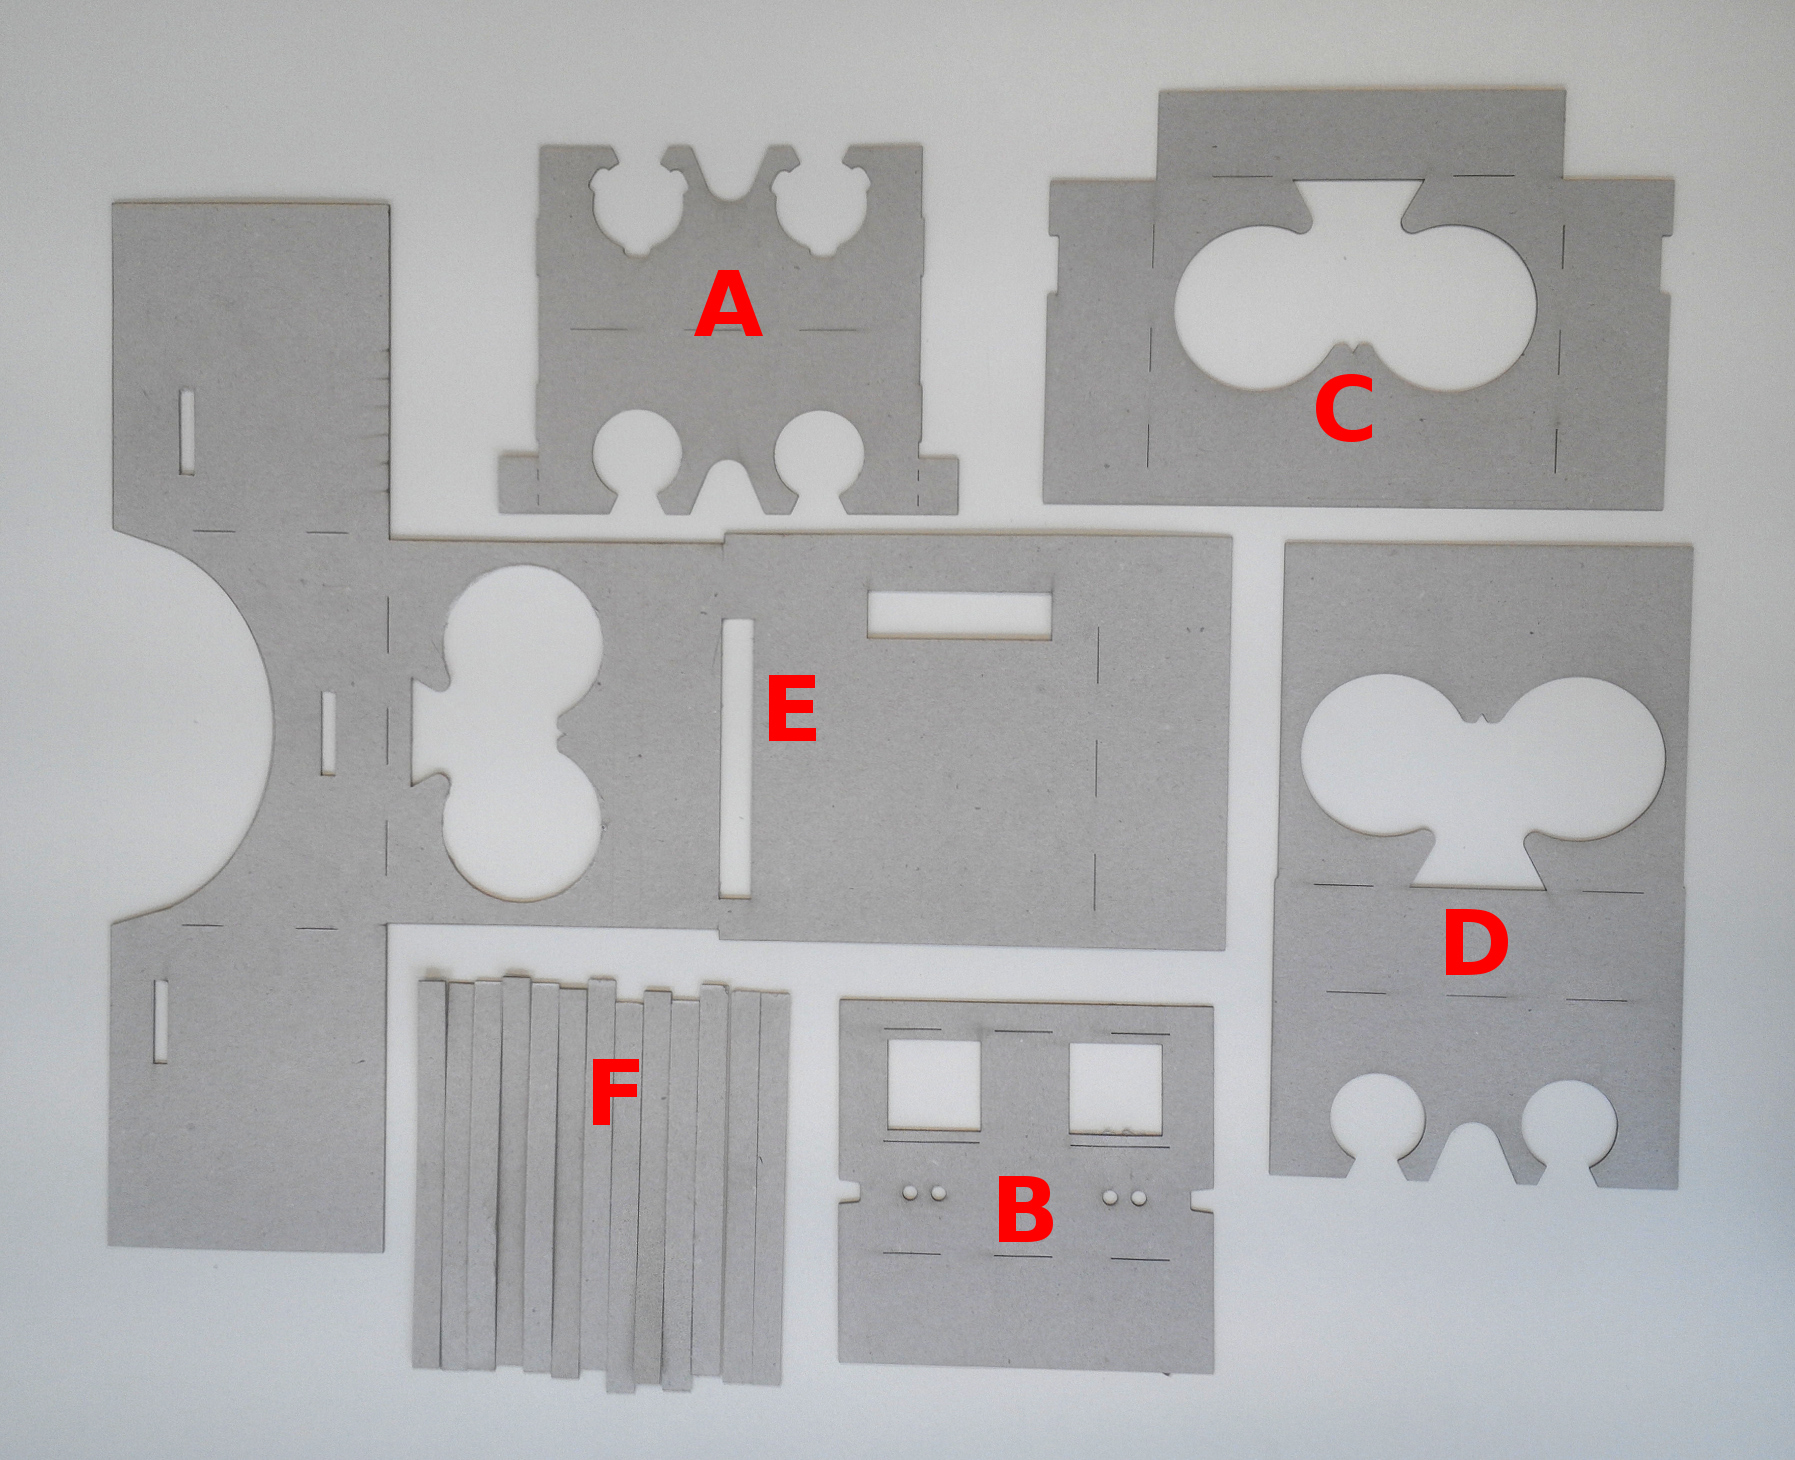
\includegraphics[width=1.0\linewidth]{all_parts}
		\caption{Cardboard pieces from A to F}
		\label{fig:screenshot001}
	\end{figure}
	\clearpage
	\item Begin with part A. For this purpose, bend the provided edges of the part (see figure \ref{fig:screenshot002}). Insert the lenses into the device (see figure \ref{fig:screenshot003}), making sure that the larger curvature of the lenses is facing the other round aperture and press firmly. Glue the part together (see figure \ref{fig:screenshot004}). Finally, their part should look like in figure \ref{fig:screenshot005}.
	\begin{figure}[htb]
		\centering
		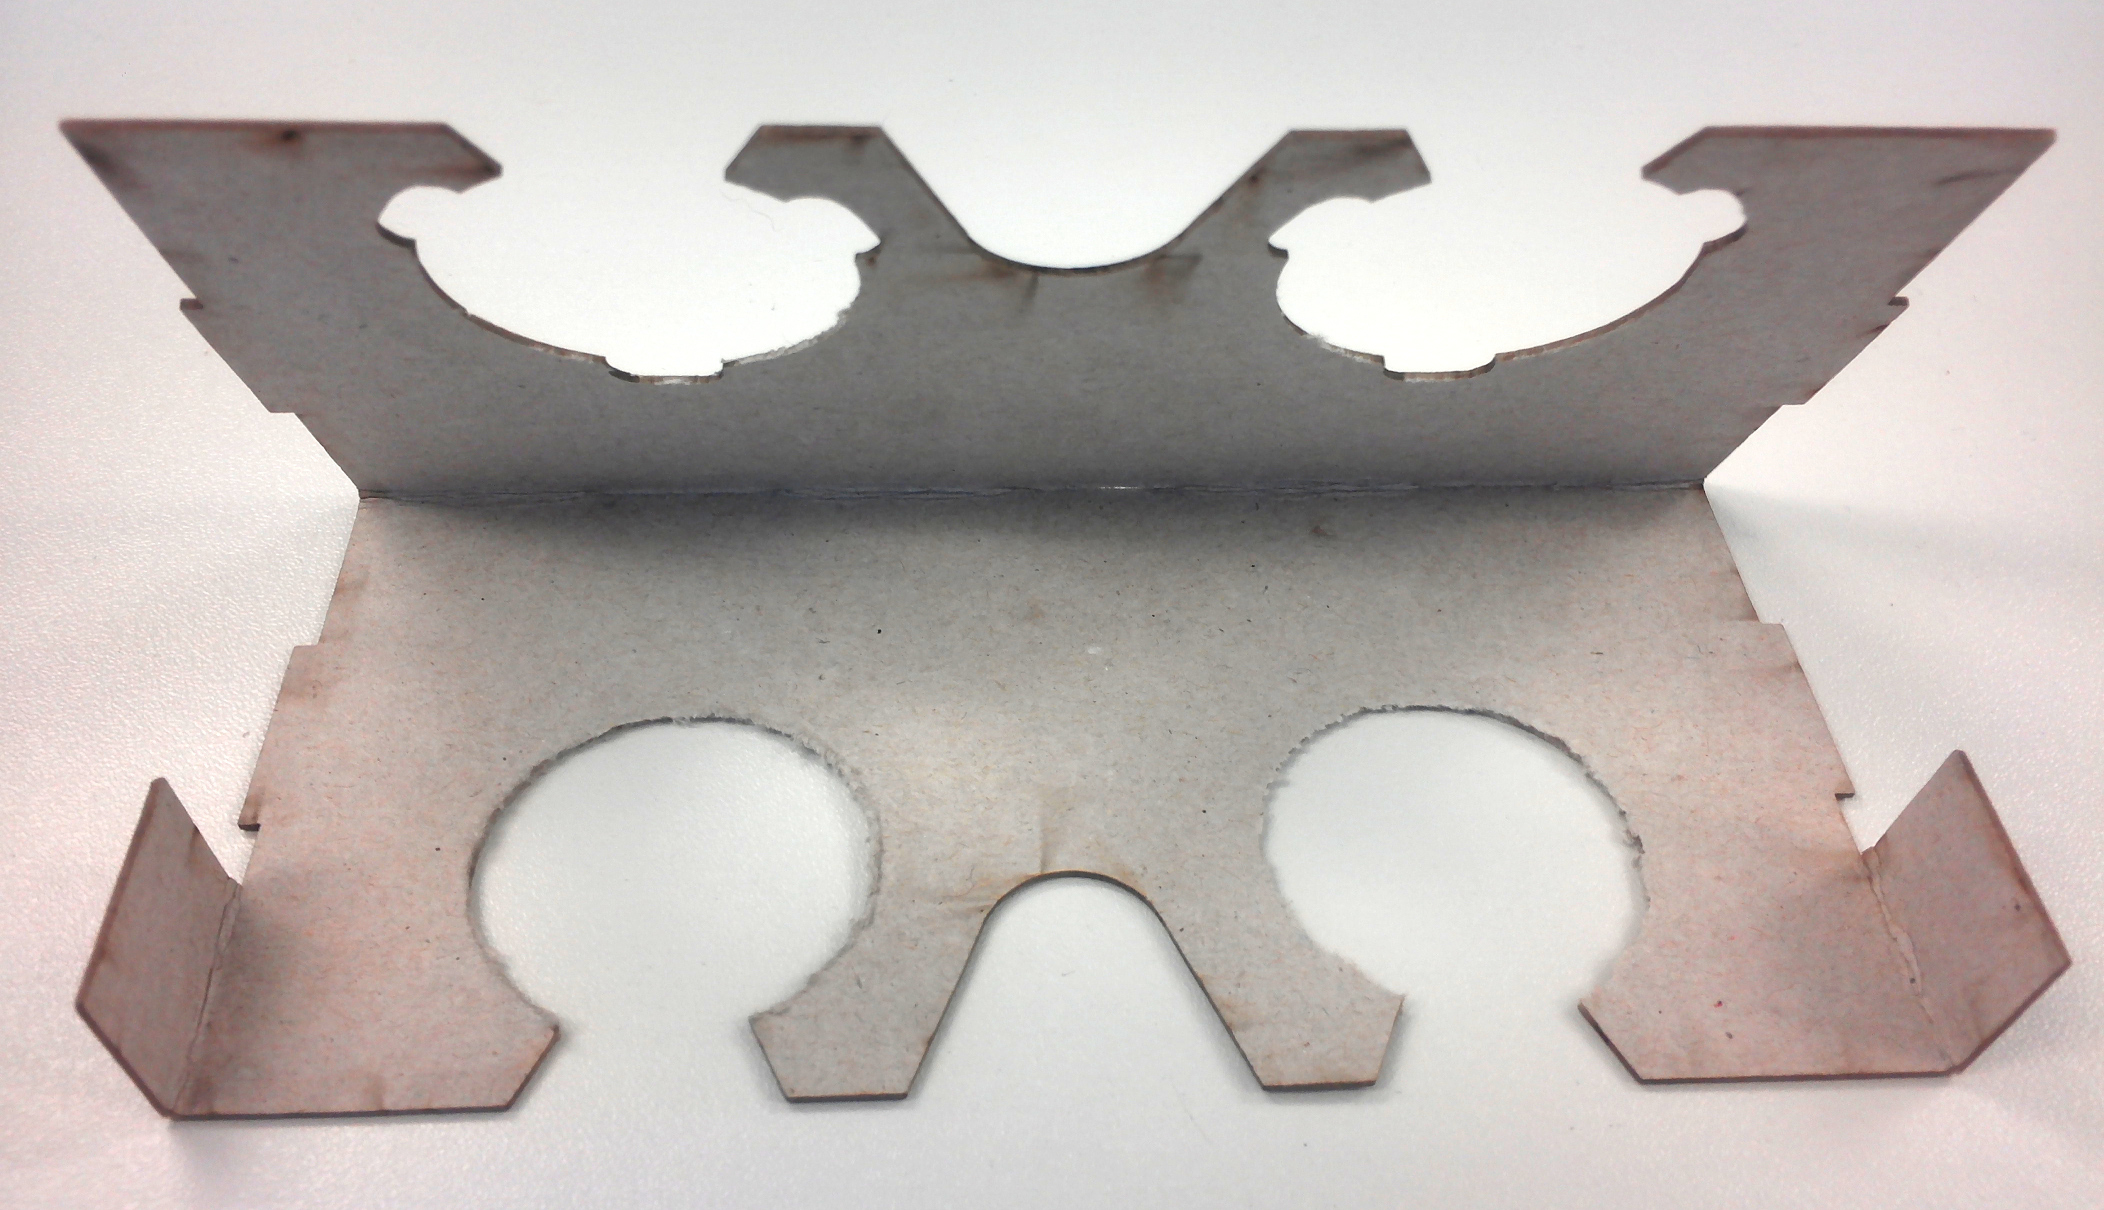
\includegraphics[width=0.7\linewidth]{partA01}
		\caption{Creased edges part A}
		\label{fig:screenshot002}
	\end{figure}
	\begin{figure}[htb]
		\centering
		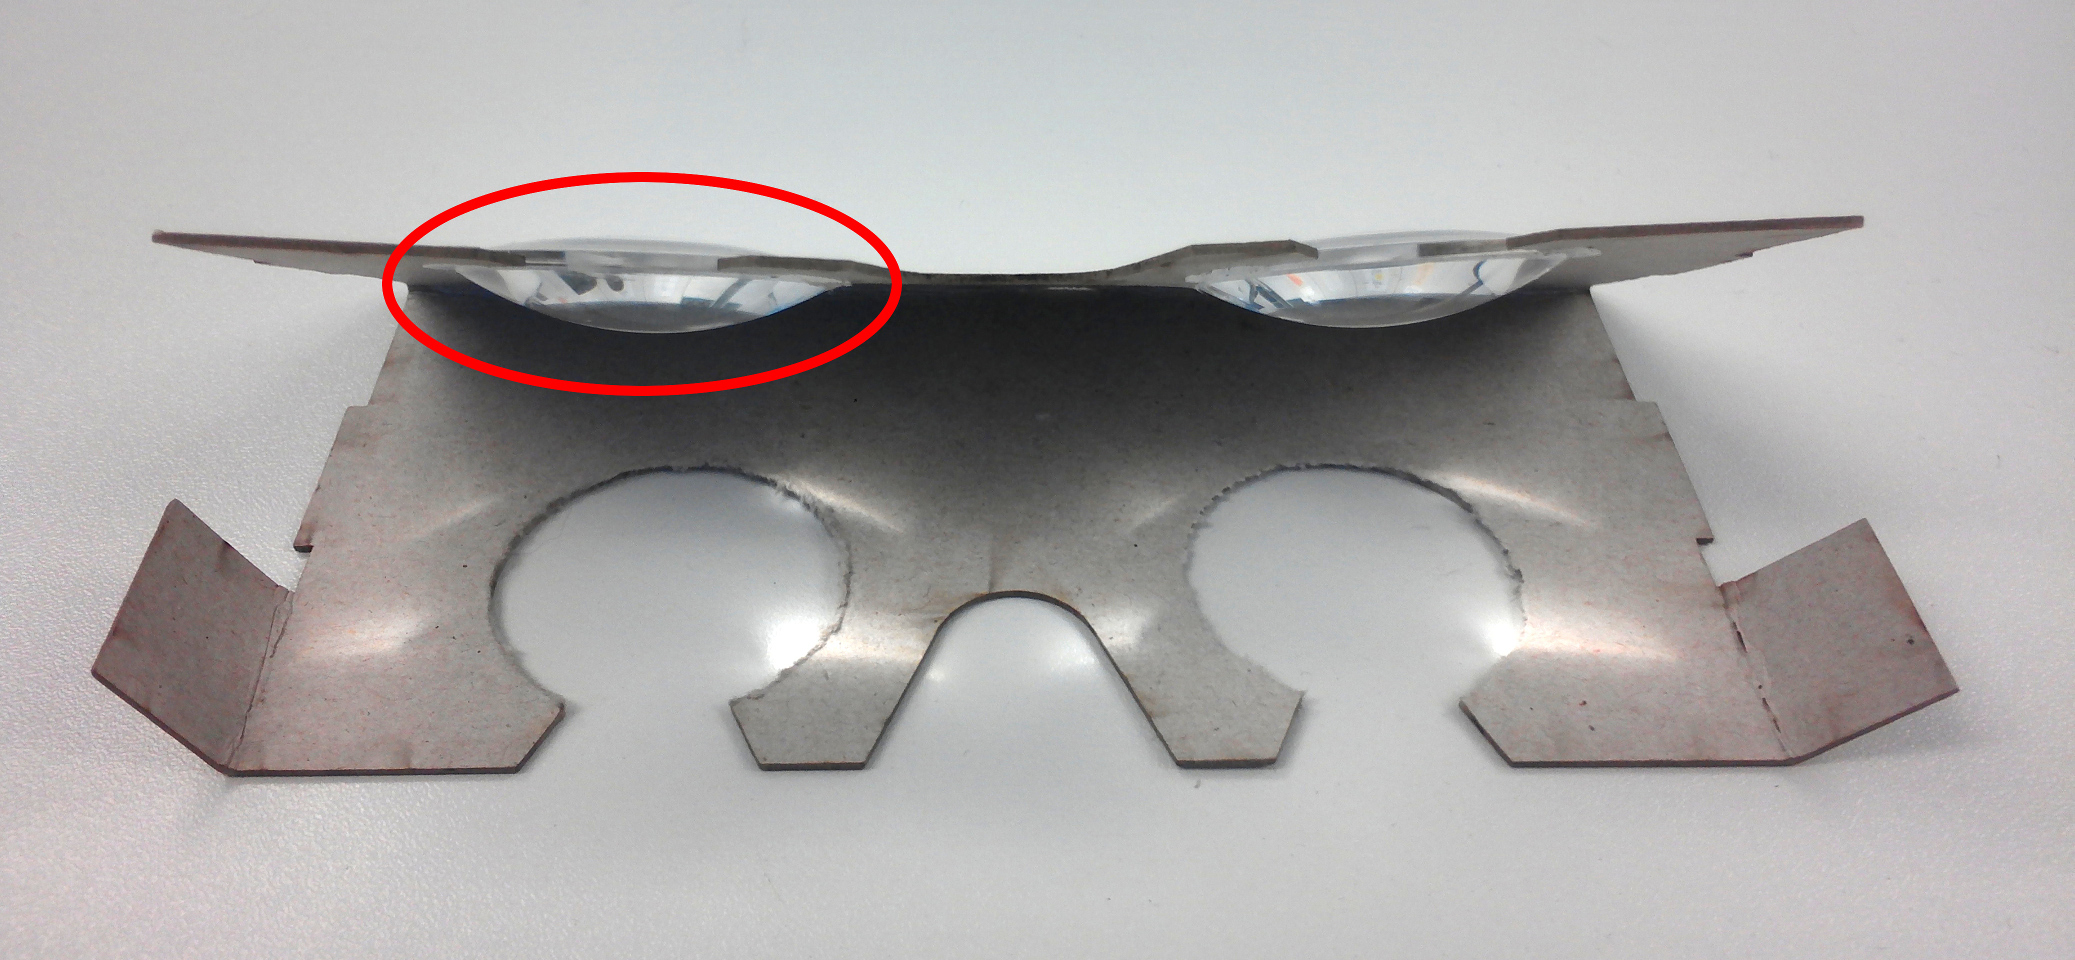
\includegraphics[width=0.7\linewidth]{partA02}
		\caption{Insert the lenses}
		\label{fig:screenshot003}
	\end{figure}
	\begin{figure}[htb]
		\centering
		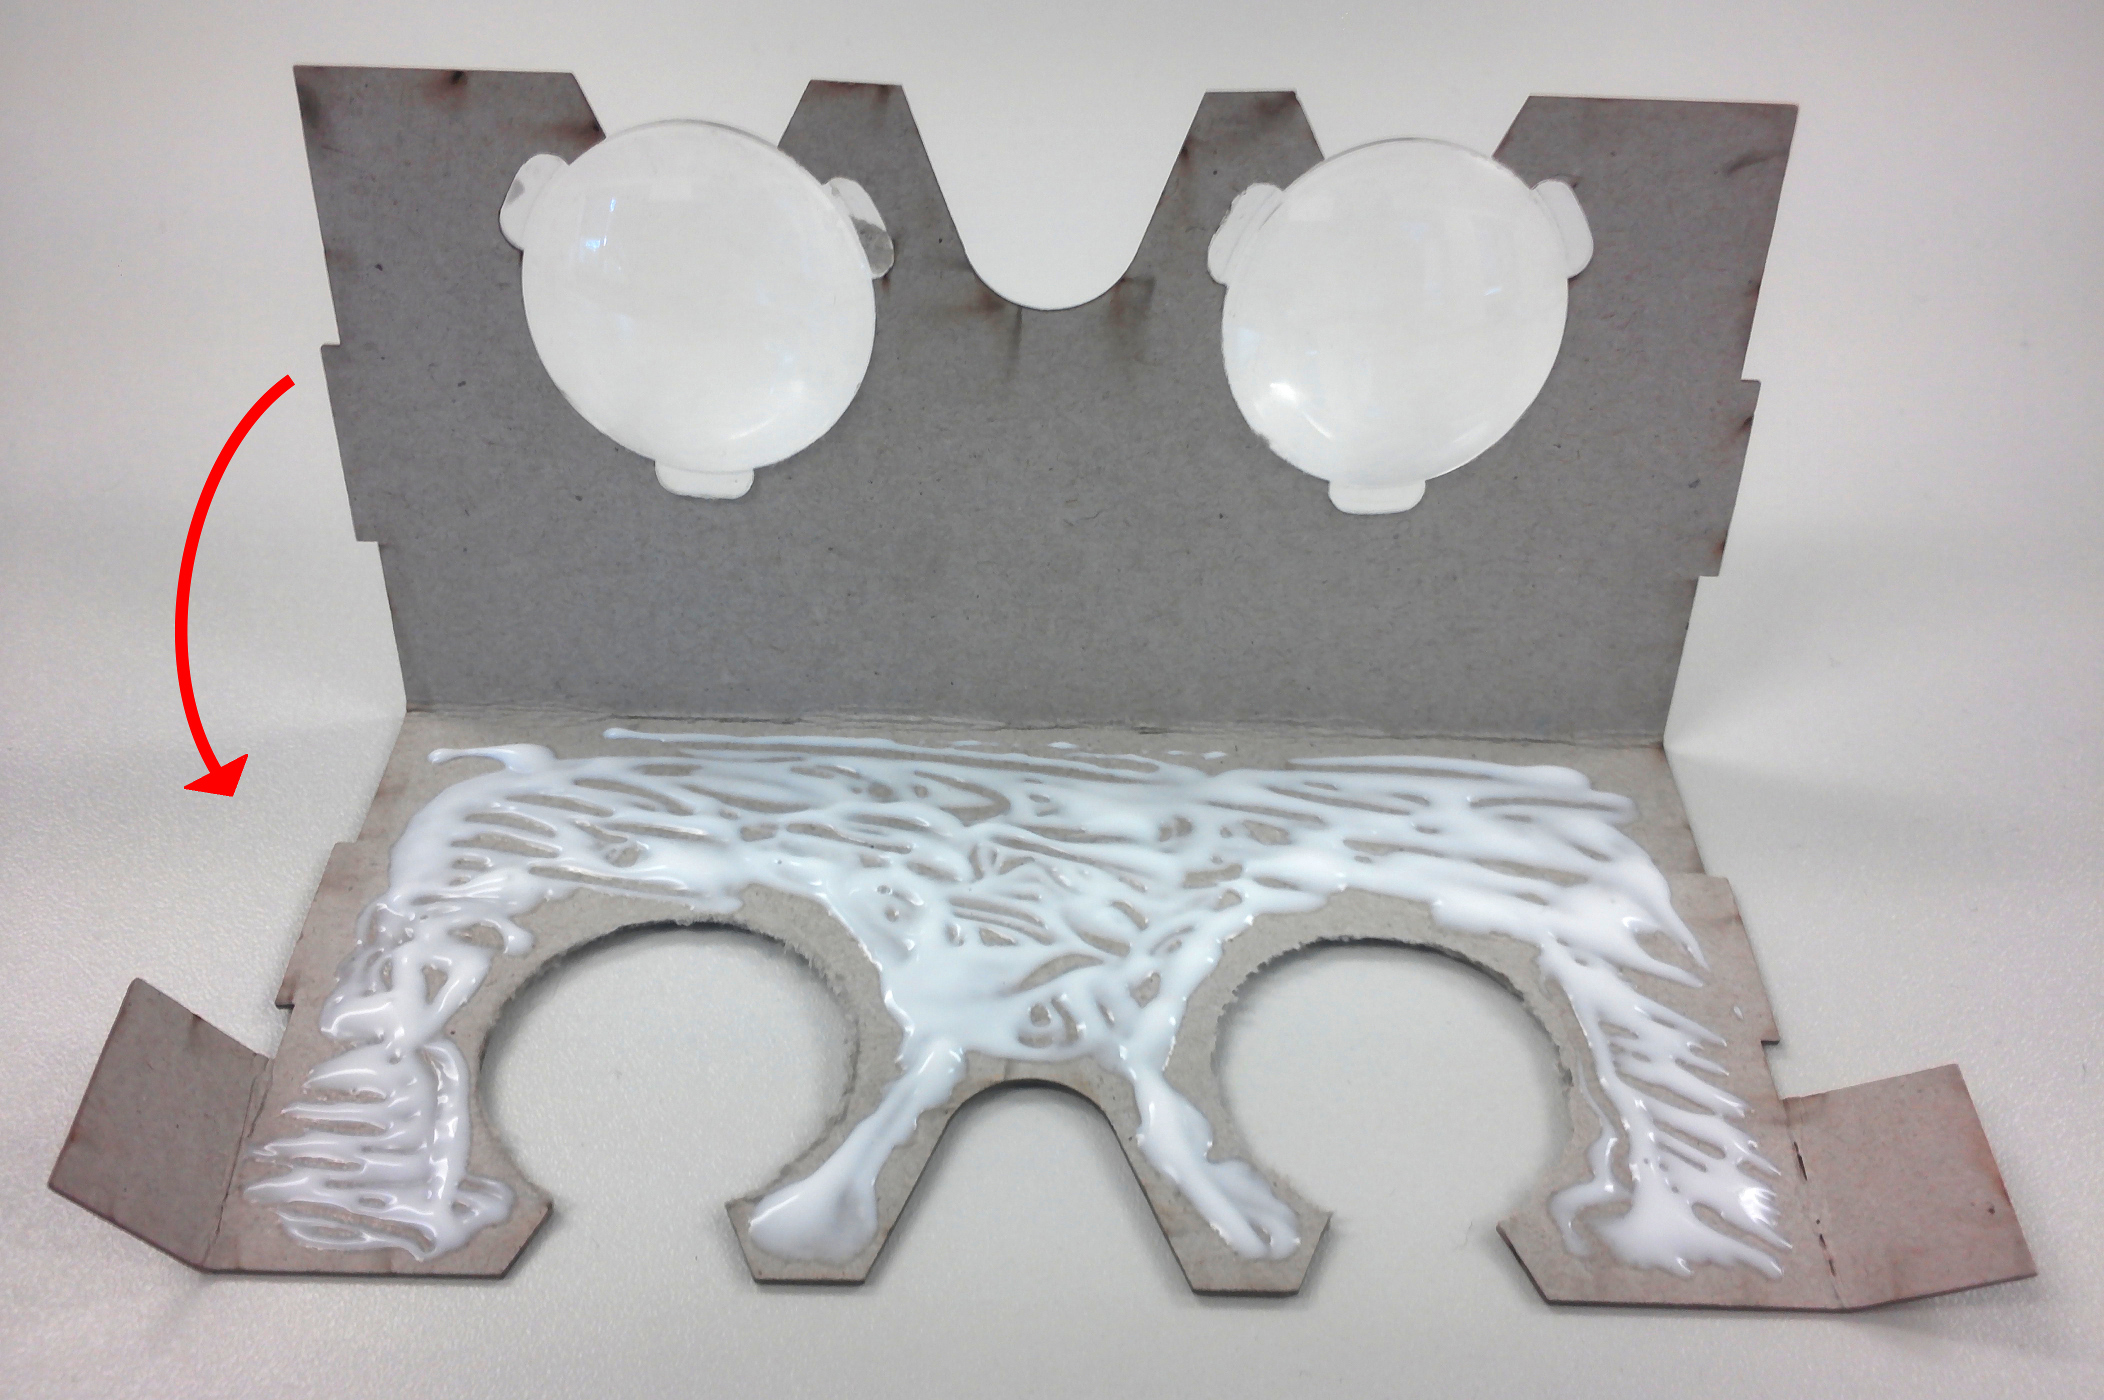
\includegraphics[width=0.7\linewidth]{partA03}
		\caption{Glueing the part A}
		\label{fig:screenshot004}
	\end{figure}
	\begin{figure}[htb]
		\centering
		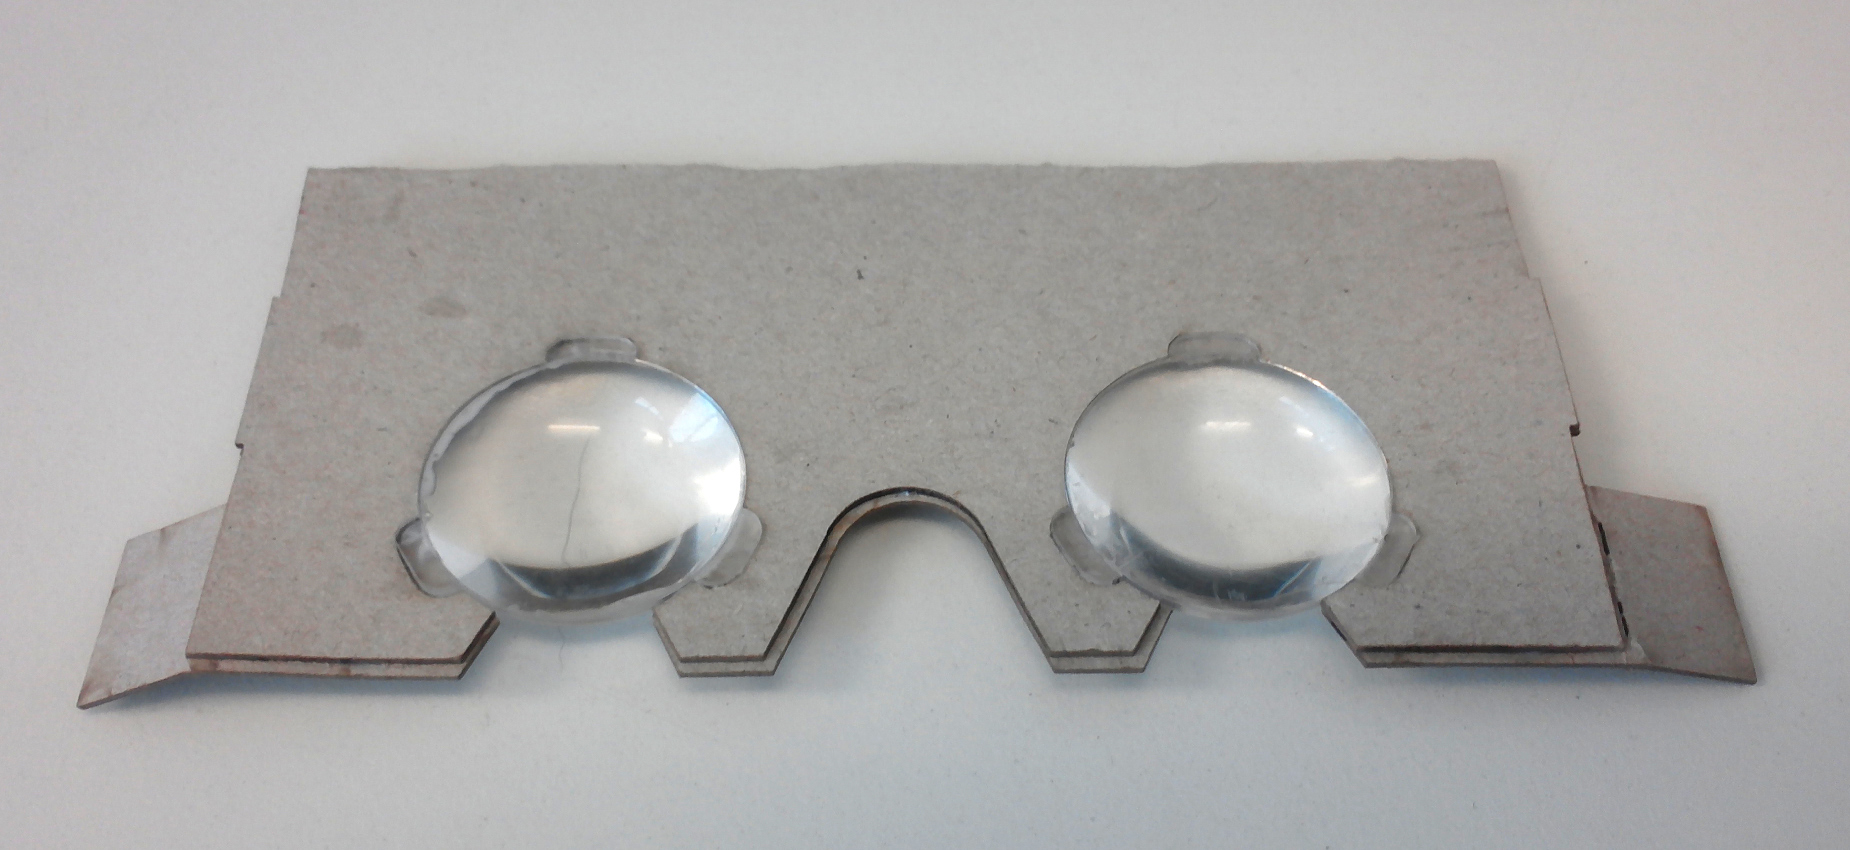
\includegraphics[width=0.7\linewidth]{partA04}
		\caption{Final result of part A}
		\label{fig:screenshot005}
	\end{figure}
	\clearpage
	\item Continue with part B (see figure \ref{fig:screenshot006}). In this step, you should also bend all the creased edges (Figure \ref{fig:screenshot007}). Glue the connecting link to the other end of part B, creating a triangle like on figure \ref{fig:screenshot008}.
	\begin{figure}[htb]
		\centering
		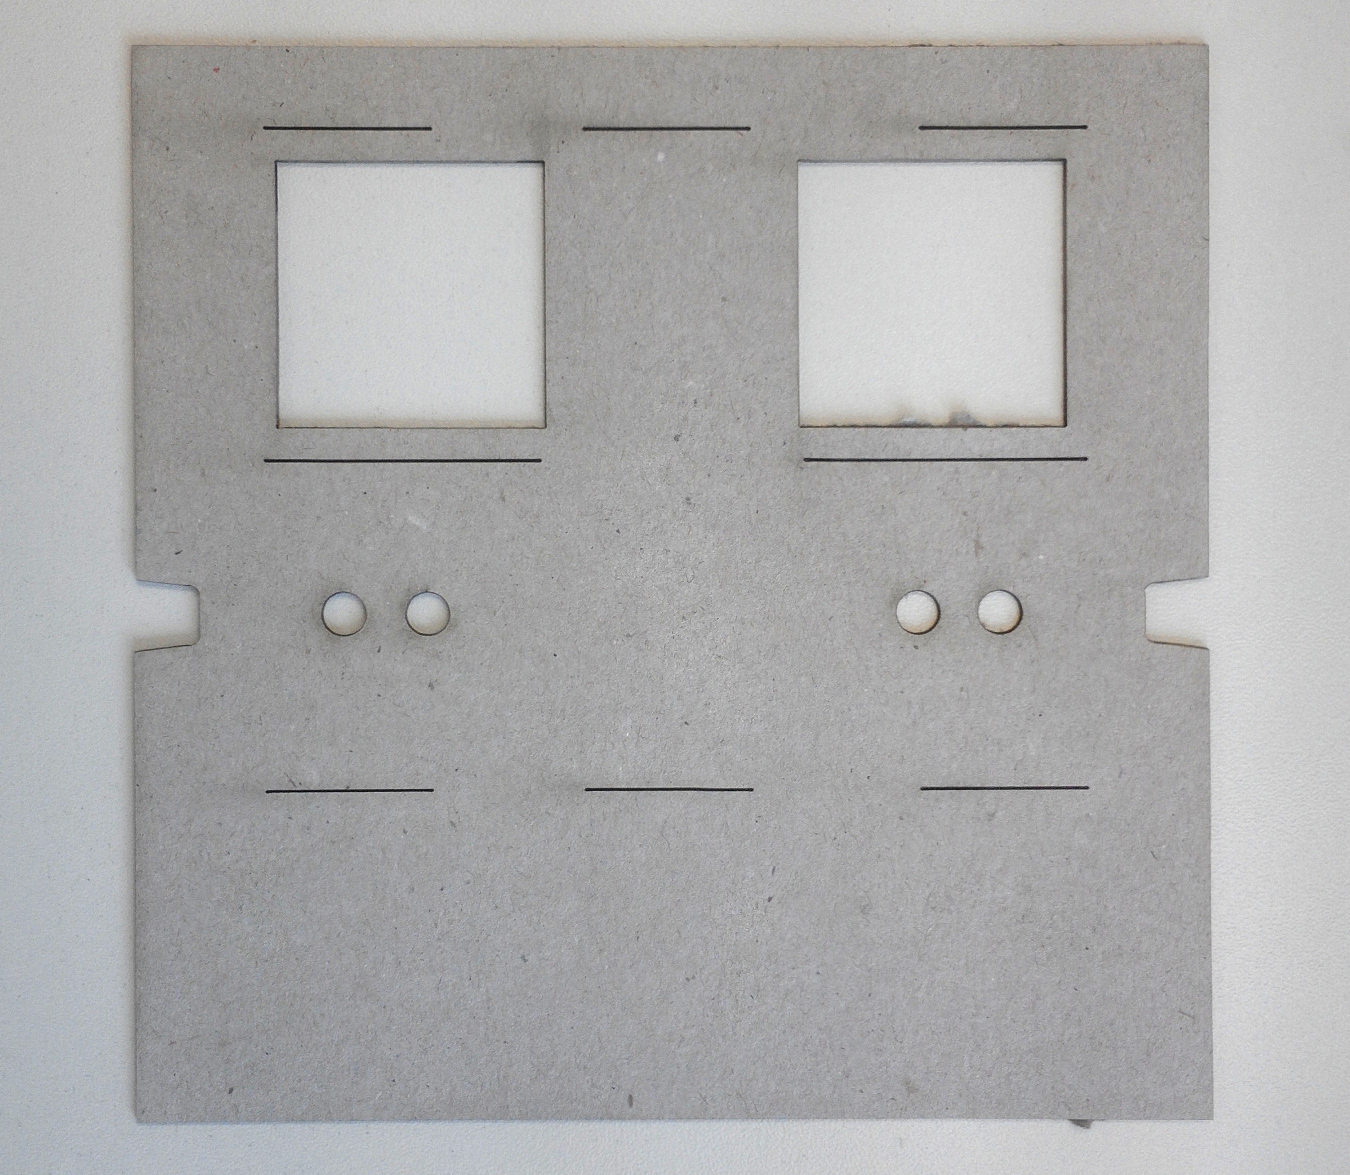
\includegraphics[width=0.8\linewidth]{partB01}
		\caption{Part B}
		\label{fig:screenshot006}
	\end{figure}
	\begin{figure}[htb]
		\centering
		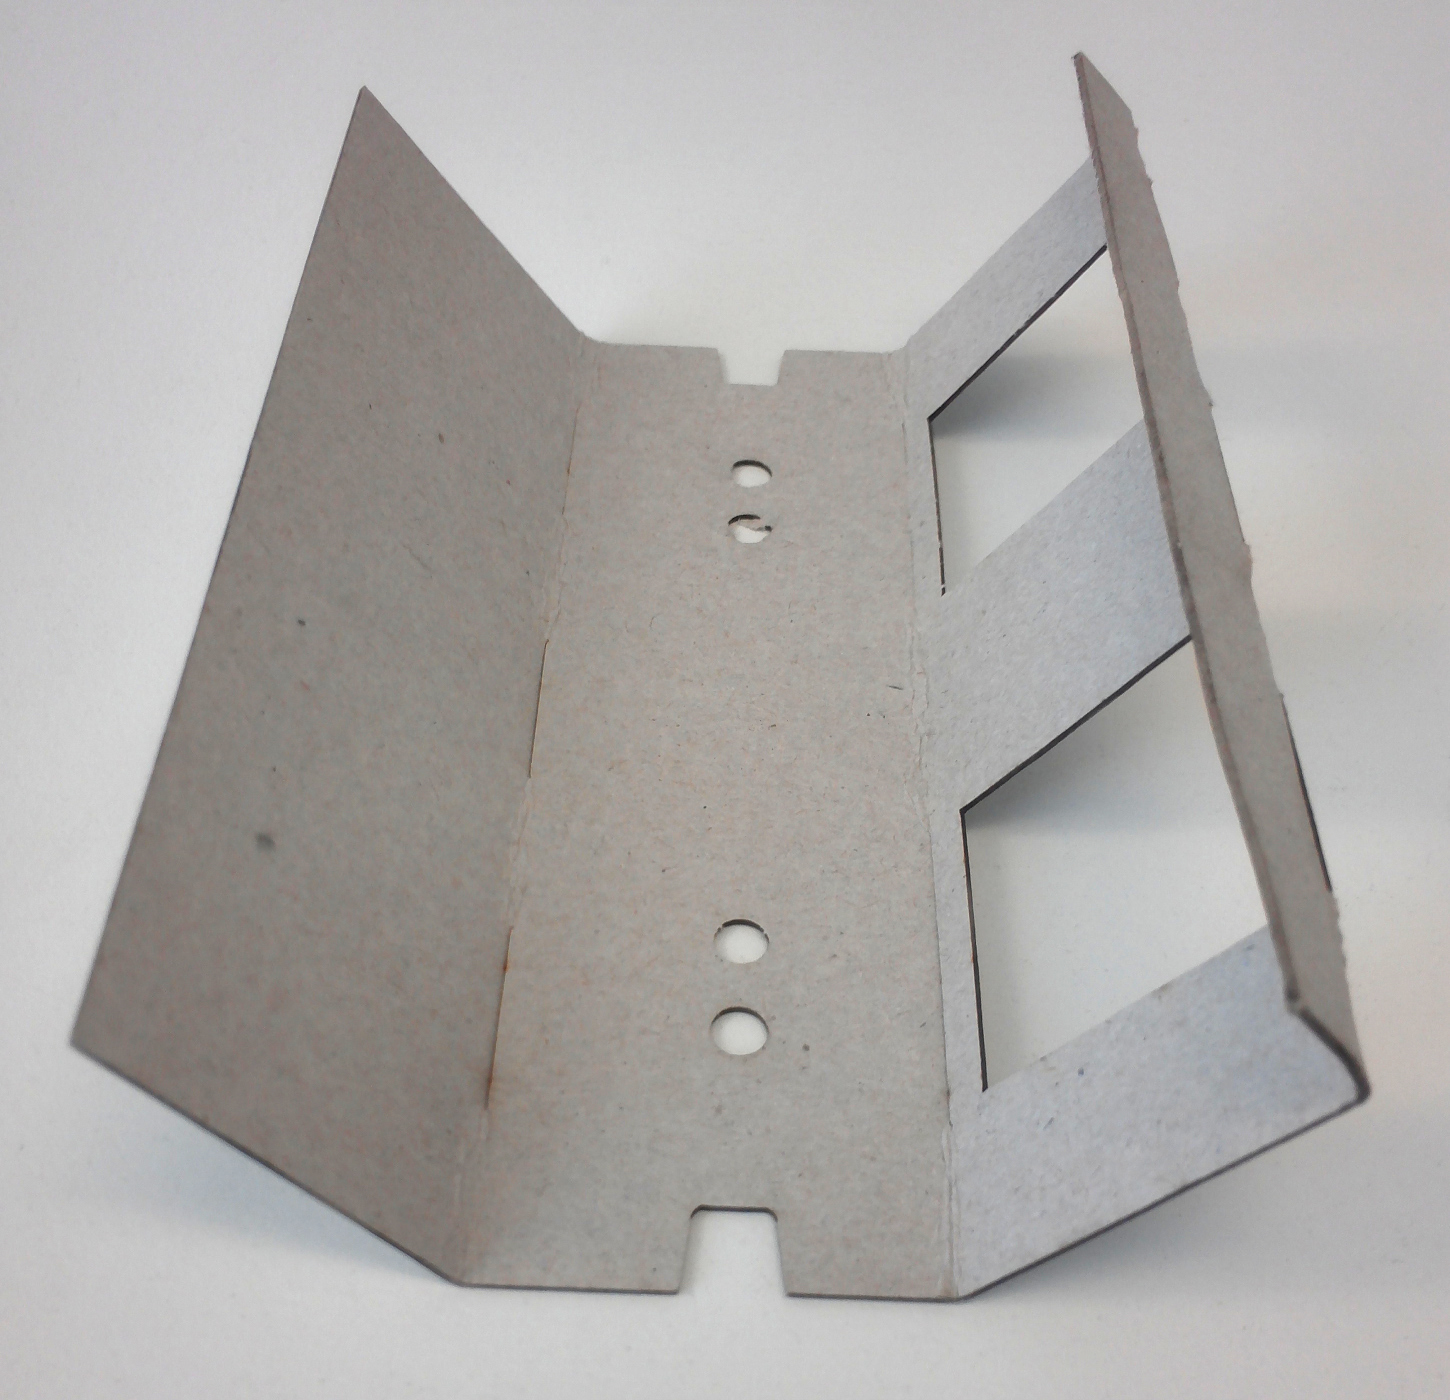
\includegraphics[width=0.5\linewidth]{partB02}
		\caption{Creased edges of part B}
		\label{fig:screenshot007}
	\end{figure}
	\begin{figure}[htb]
		\centering
		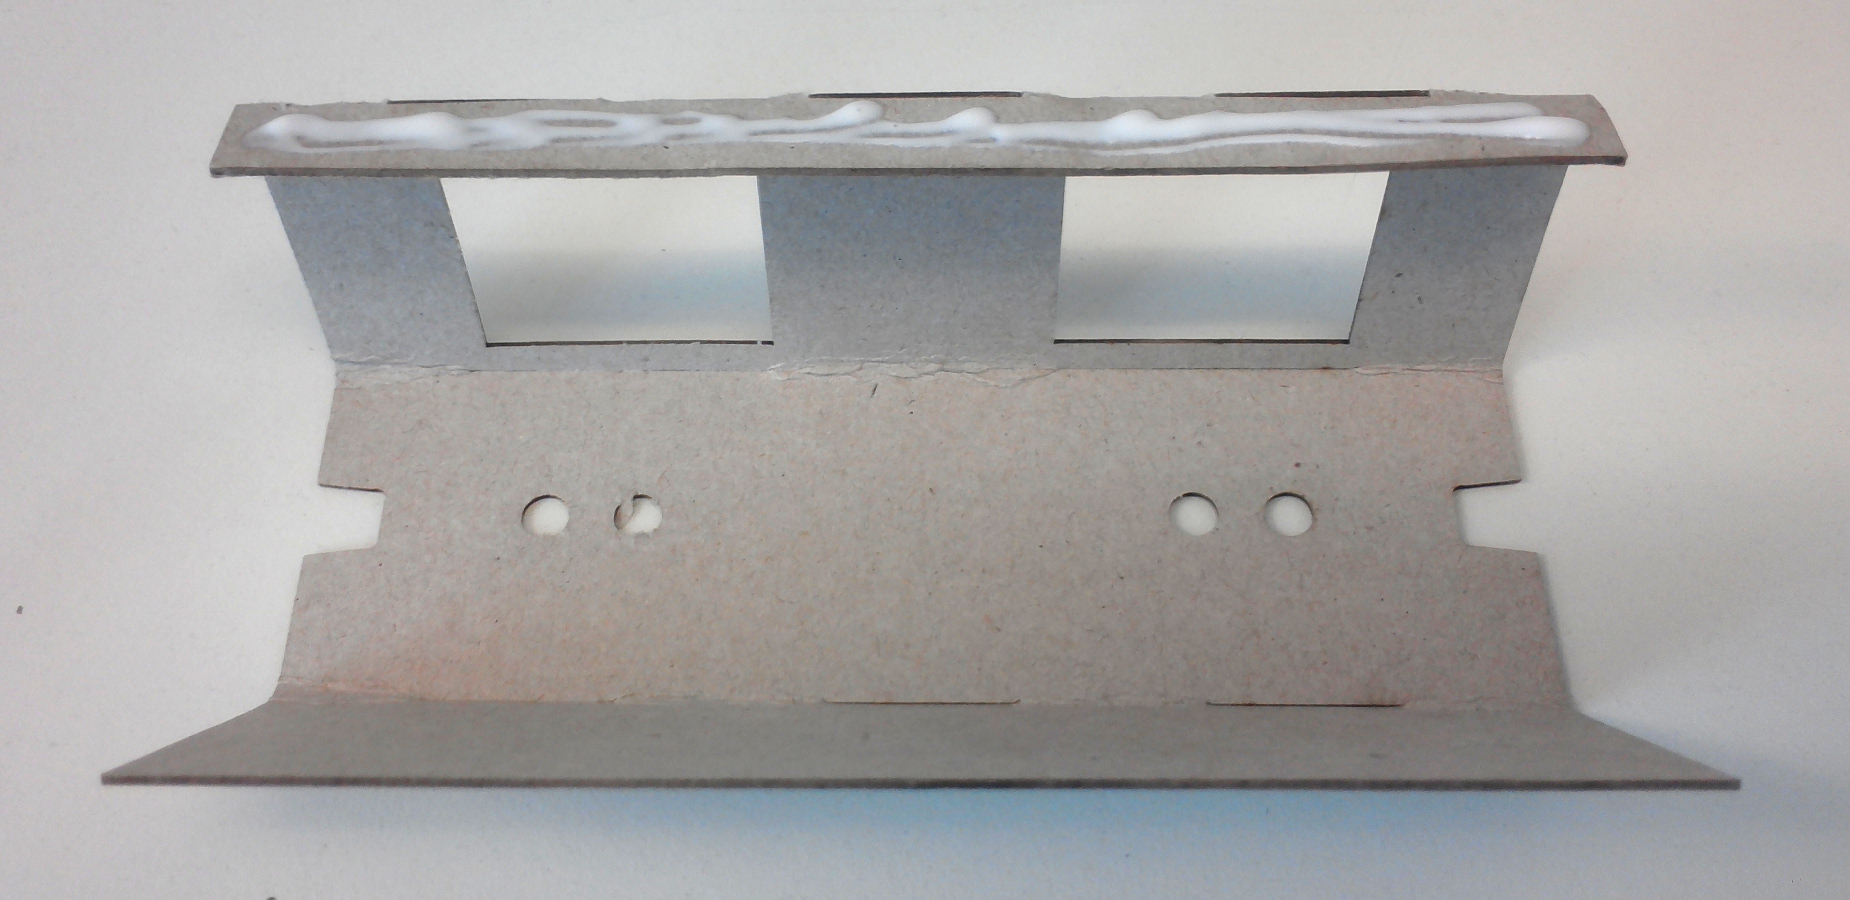
\includegraphics[width=0.6\linewidth]{partB03}\\ \vspace{2mm}
		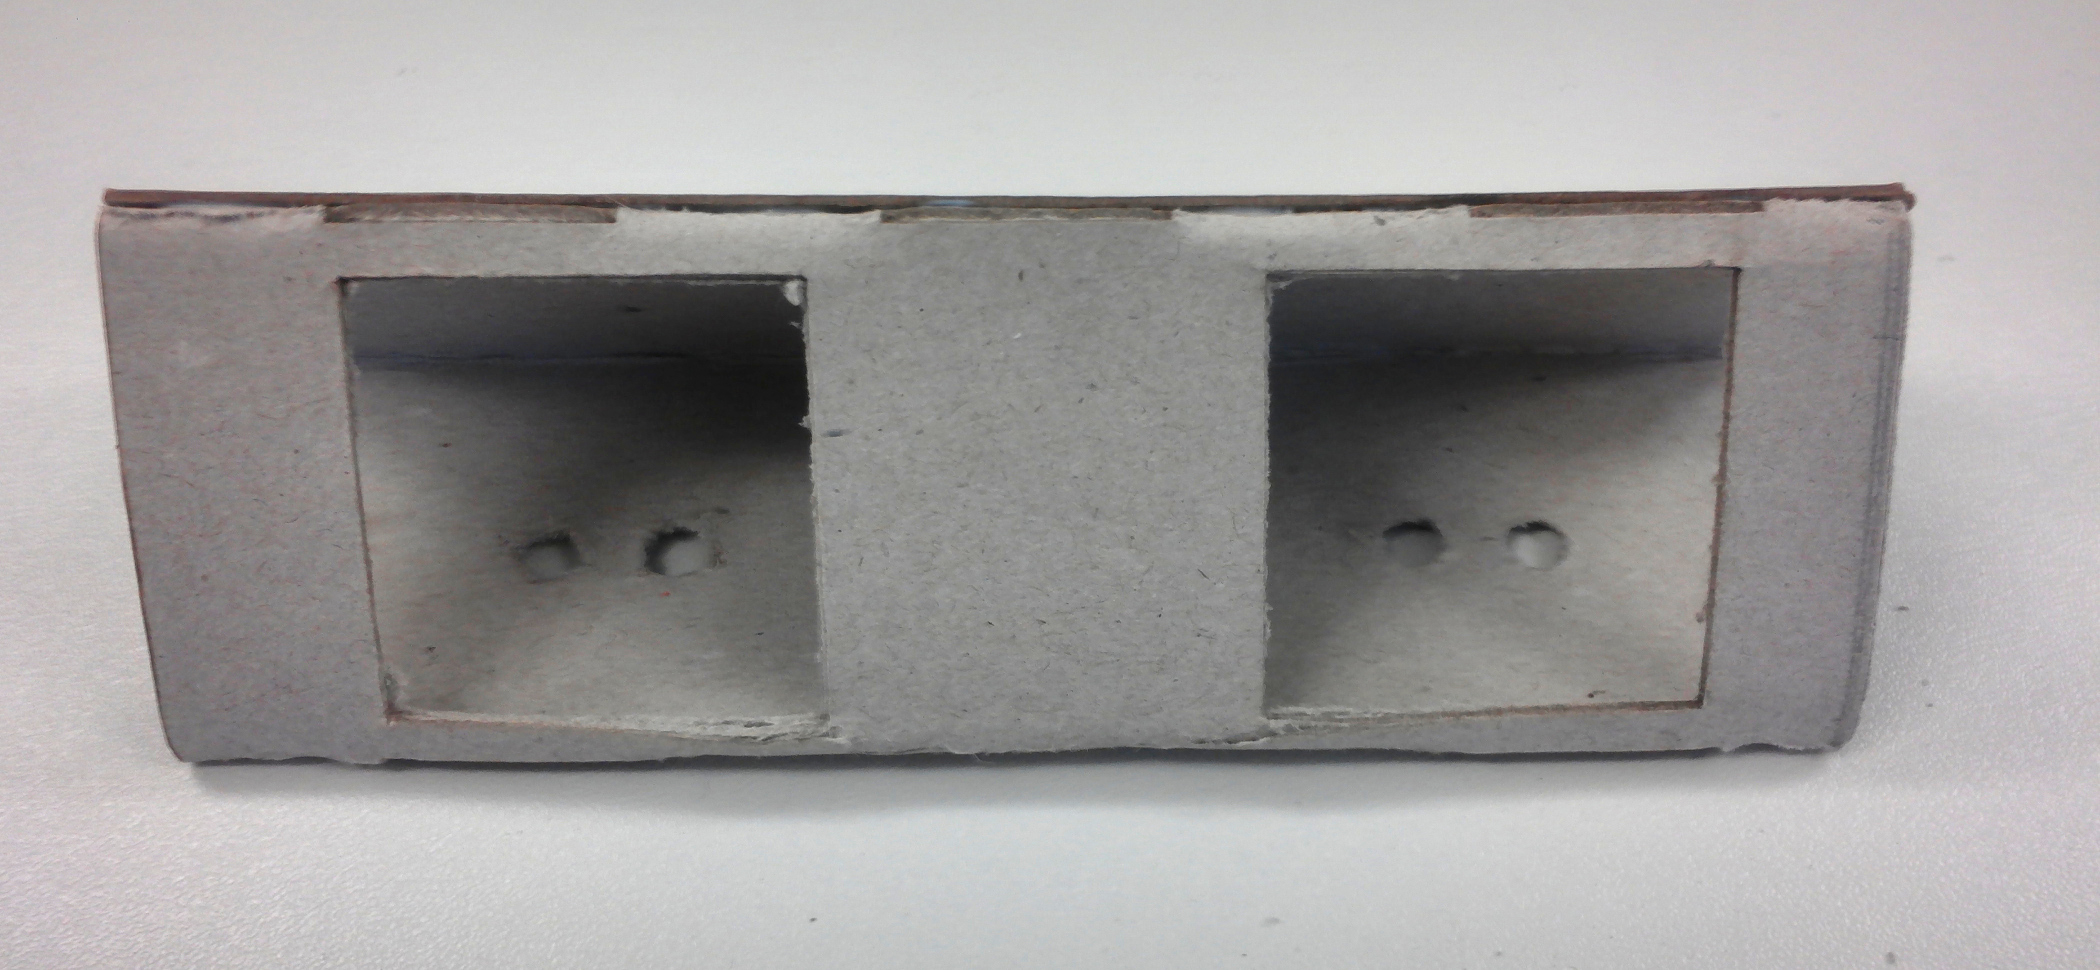
\includegraphics[width=0.6\linewidth]{partB04}
		\caption{Glueing the connecting link to other end of the part B}
		\label{fig:screenshot008}
	\end{figure}
	\clearpage
	\item Fold the creased edges of part C (see figure \ref{fig:screenshot011}). Make sure to fold the edges to the inside of part C, an engraved ``I'' marks inside of part C (see figure \ref{fig:partCmark}). Place the previously finished part A on the slots in part C (see circle on figure \ref{fig:screenshot011} and figure \ref{fig:screenshot012}). The auxiliary parts, which have been bent into part A, are now glued in the interior of part C (see figure \ref{fig:screenshot013}). The final result is a combination of part A and part C.
	\begin{figure}[htb]
		\centering
		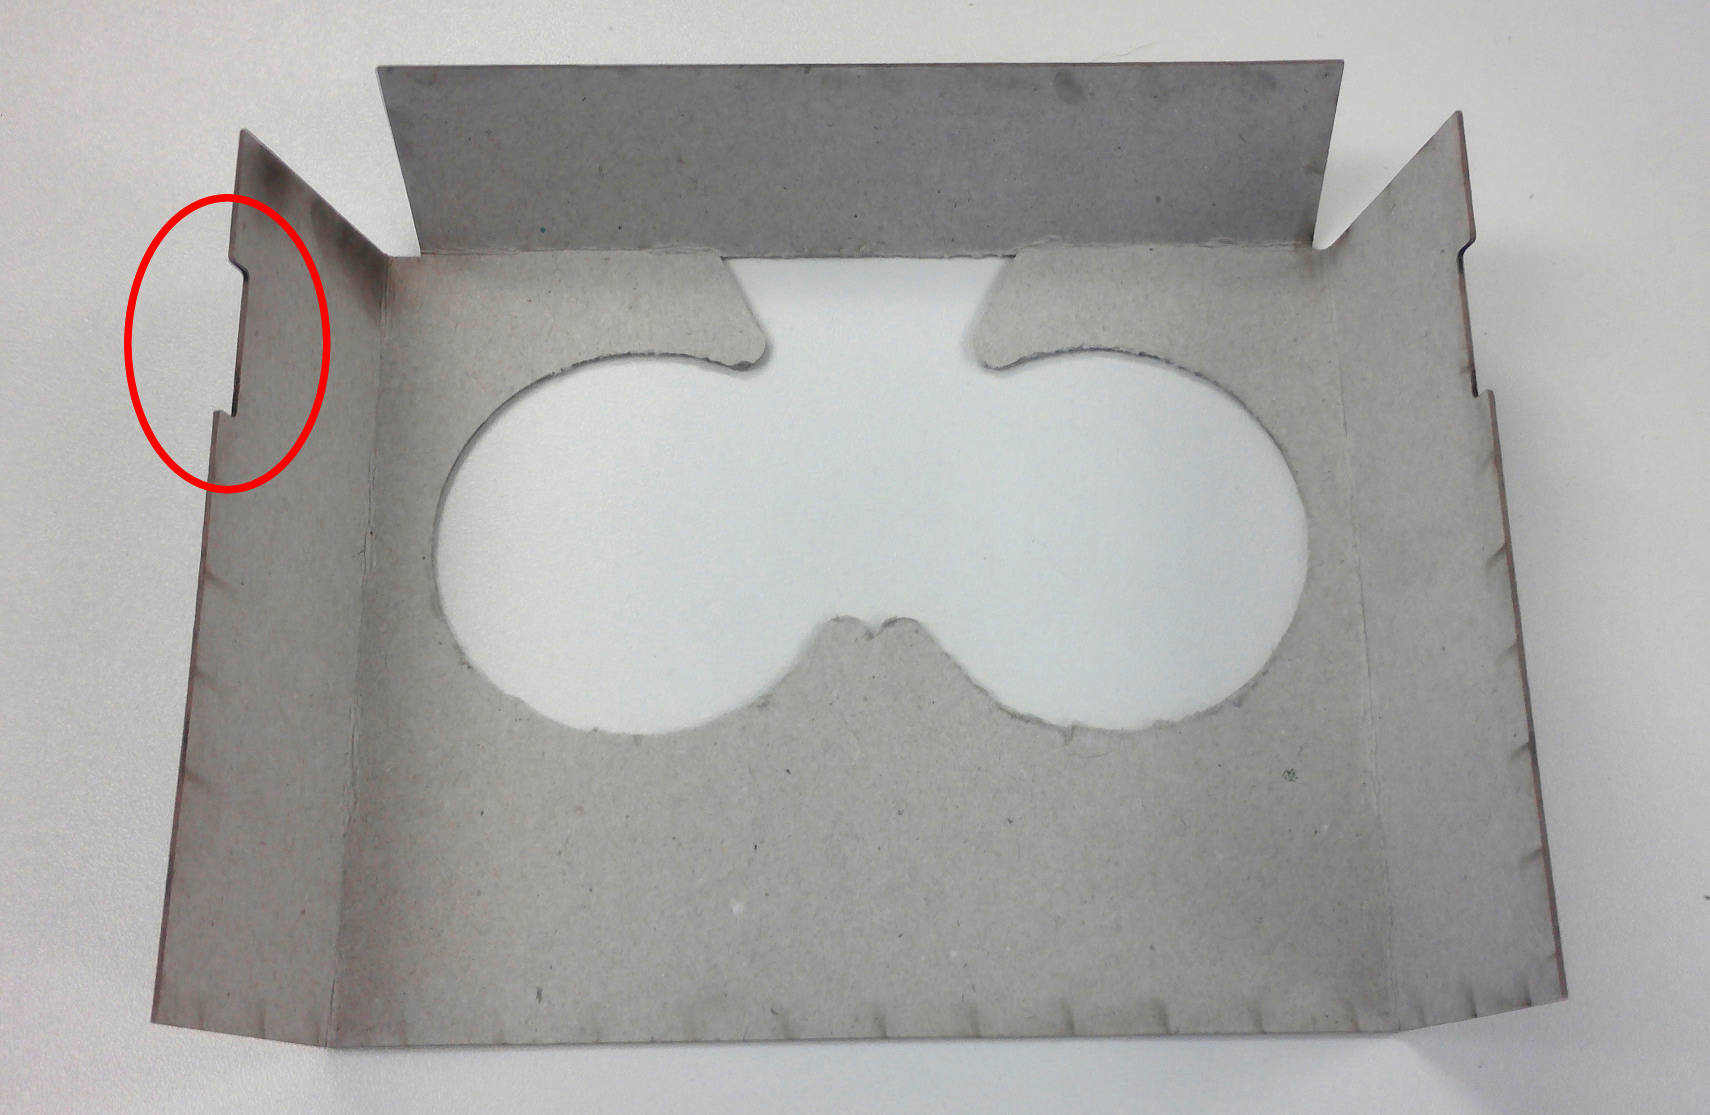
\includegraphics[width=0.8\linewidth]{partC01}
		\caption{Part C and the slots for part A}
		\label{fig:screenshot011}
	\end{figure}
	\begin{figure}[htb]
		\centering
		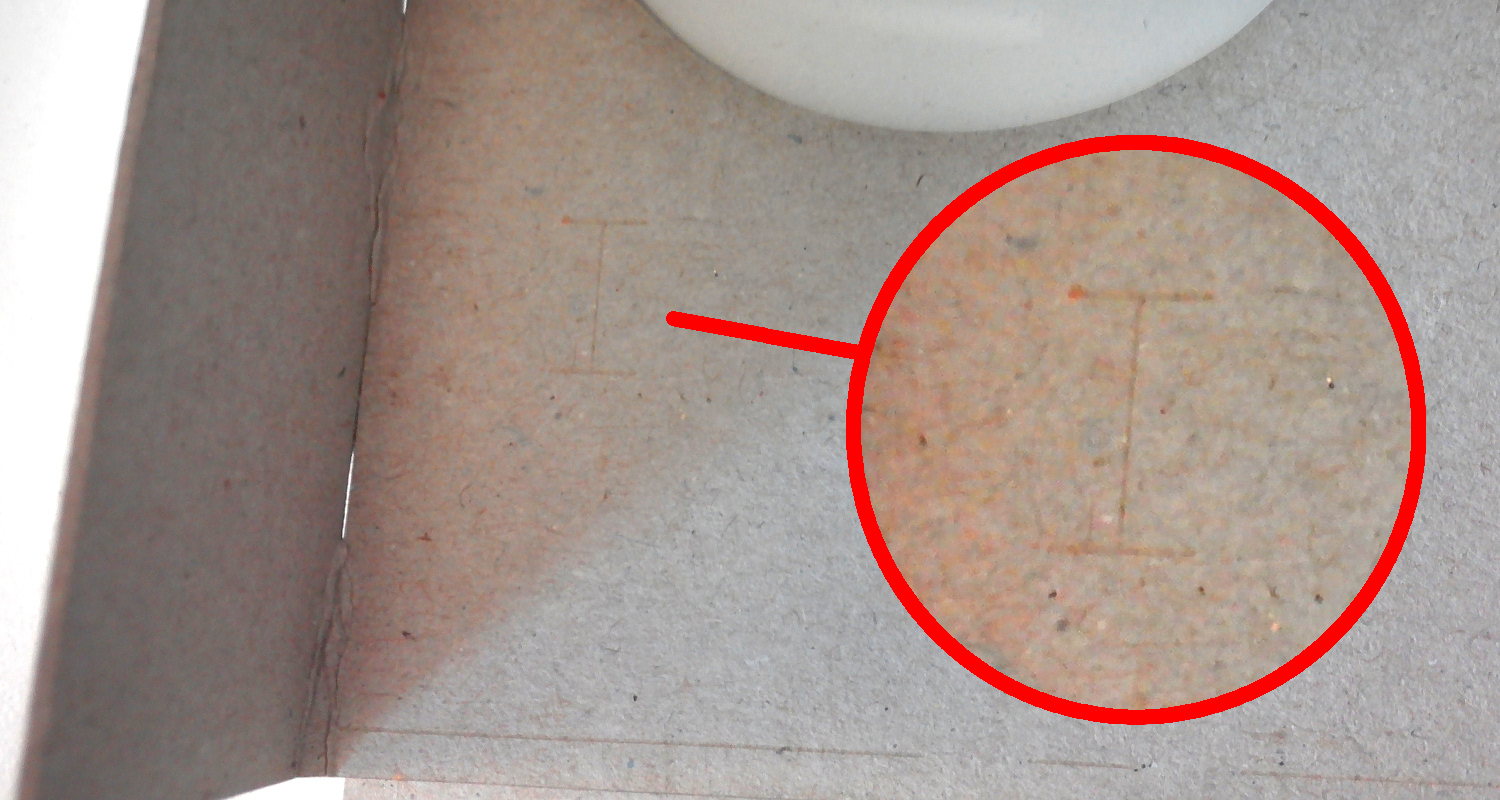
\includegraphics[width=0.6\linewidth]{partC02}
		\caption{Part C and the slots for part A}
		\label{fig:partCmark}
	\end{figure}
	\begin{figure}[htb]
		\centering
		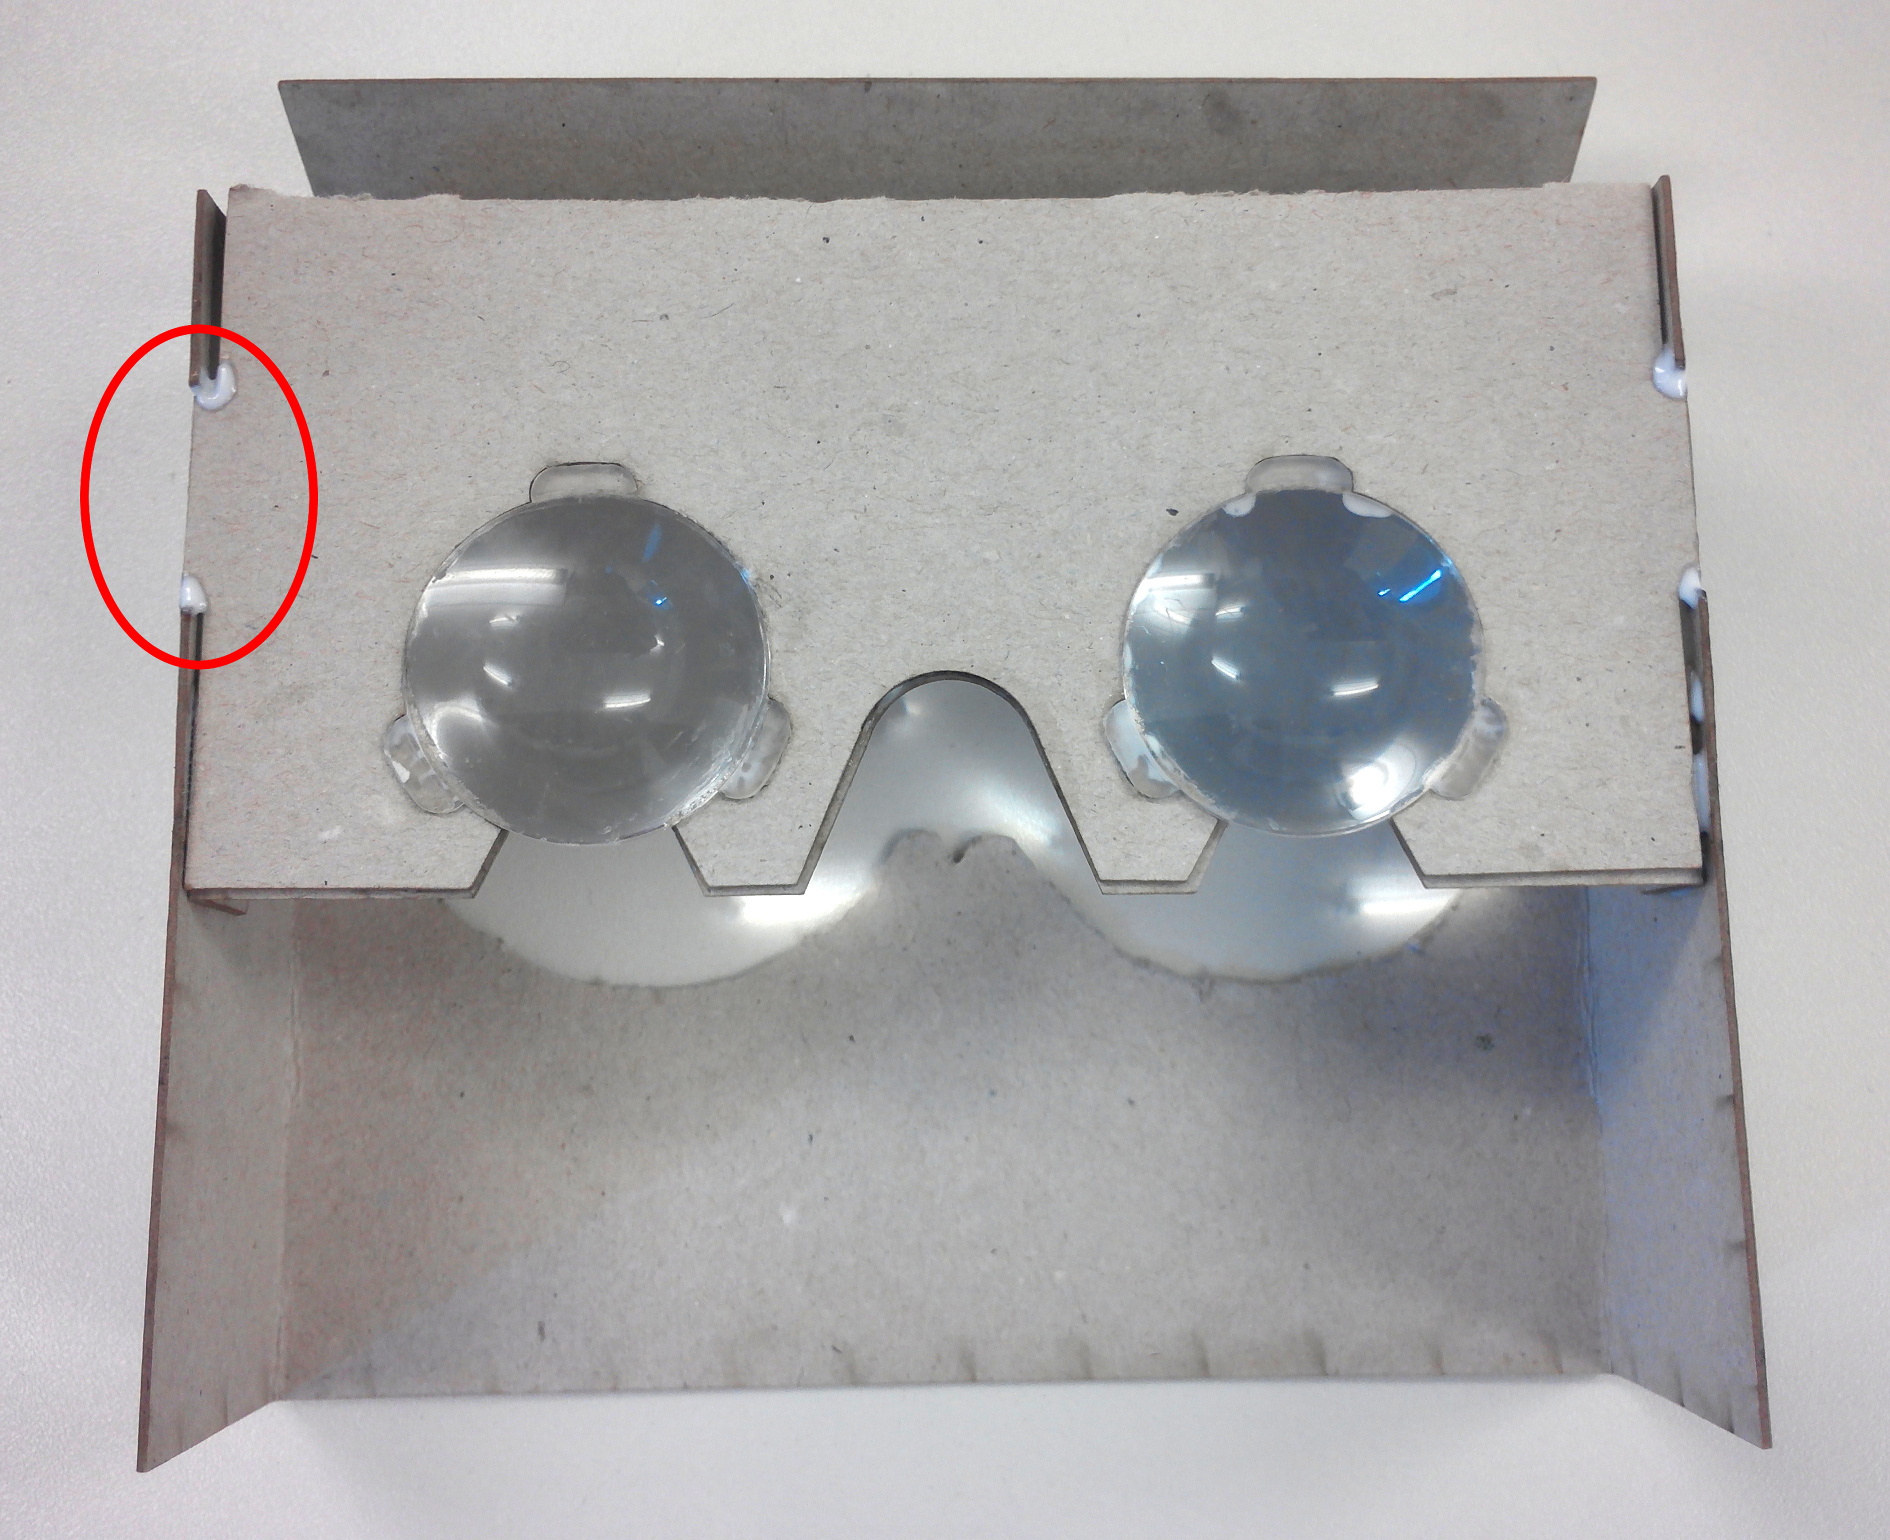
\includegraphics[width=0.7\linewidth]{partAC01}
		\caption{Part A in the slots of part C}
		\label{fig:screenshot012}
	\end{figure}\\
	\begin{figure}[htb]
		\centering
		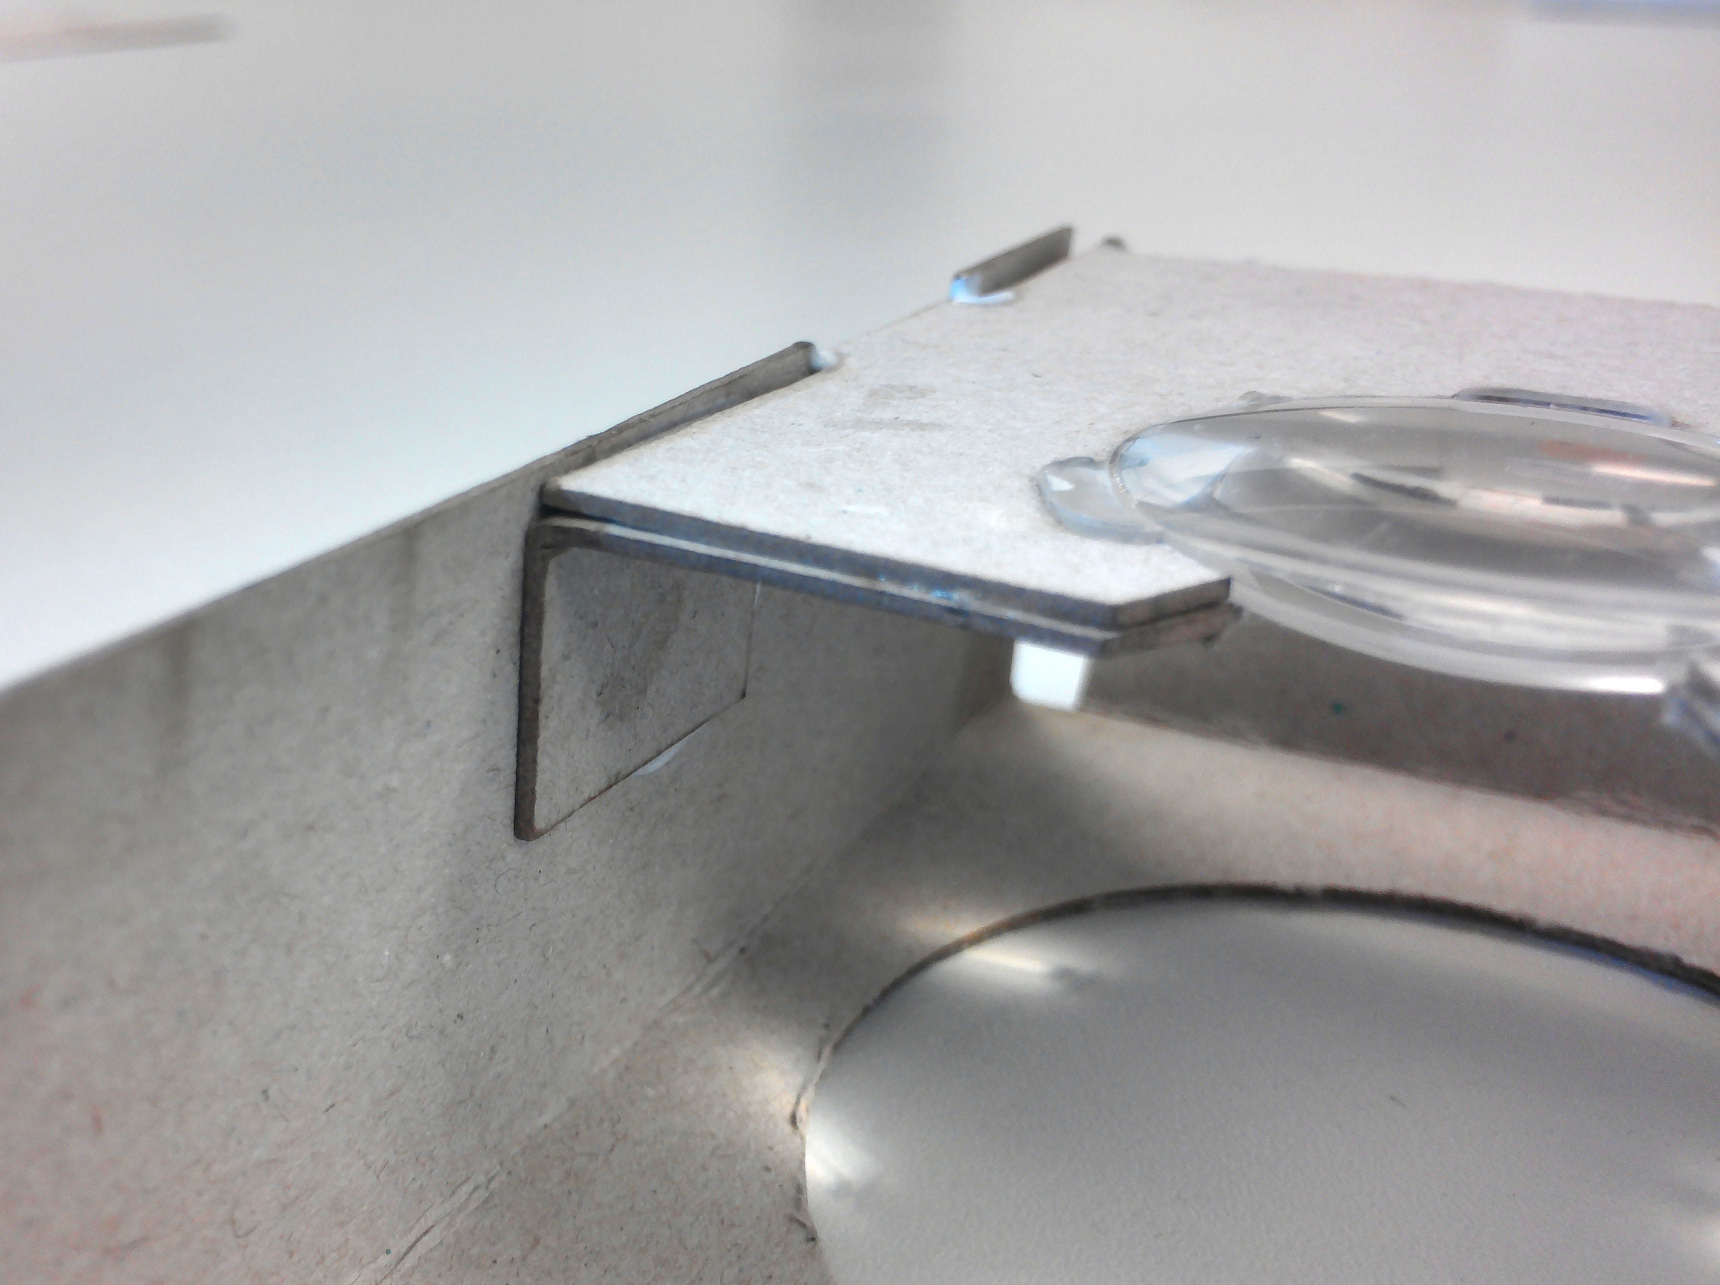
\includegraphics[width=0.7\linewidth]{partAC02}
		\caption{Attached the auxiliary pieces of part A to part C}
		\label{fig:screenshot013}
	\end{figure}
	\clearpage
	\item Now the result generated in step 4 is combined with part D (see figure \ref{fig:screenshot014}). To do this, place the combination of A and C on the part D and glue them together. Then glue the top side of both parts together and place the side with the round aperture of part D on the side with the lenses of the A/C combination. The process is shown in figure \ref{fig:screenshot016}.
	\begin{figure}[htb]
		\centering
		\includegraphics[width=0.85\linewidth]{partACD01}
		\caption{Left part D, right part A in combination with part C}
		\label{fig:screenshot014}
	\end{figure}
	\begin{figure}[htb]
		\centering
		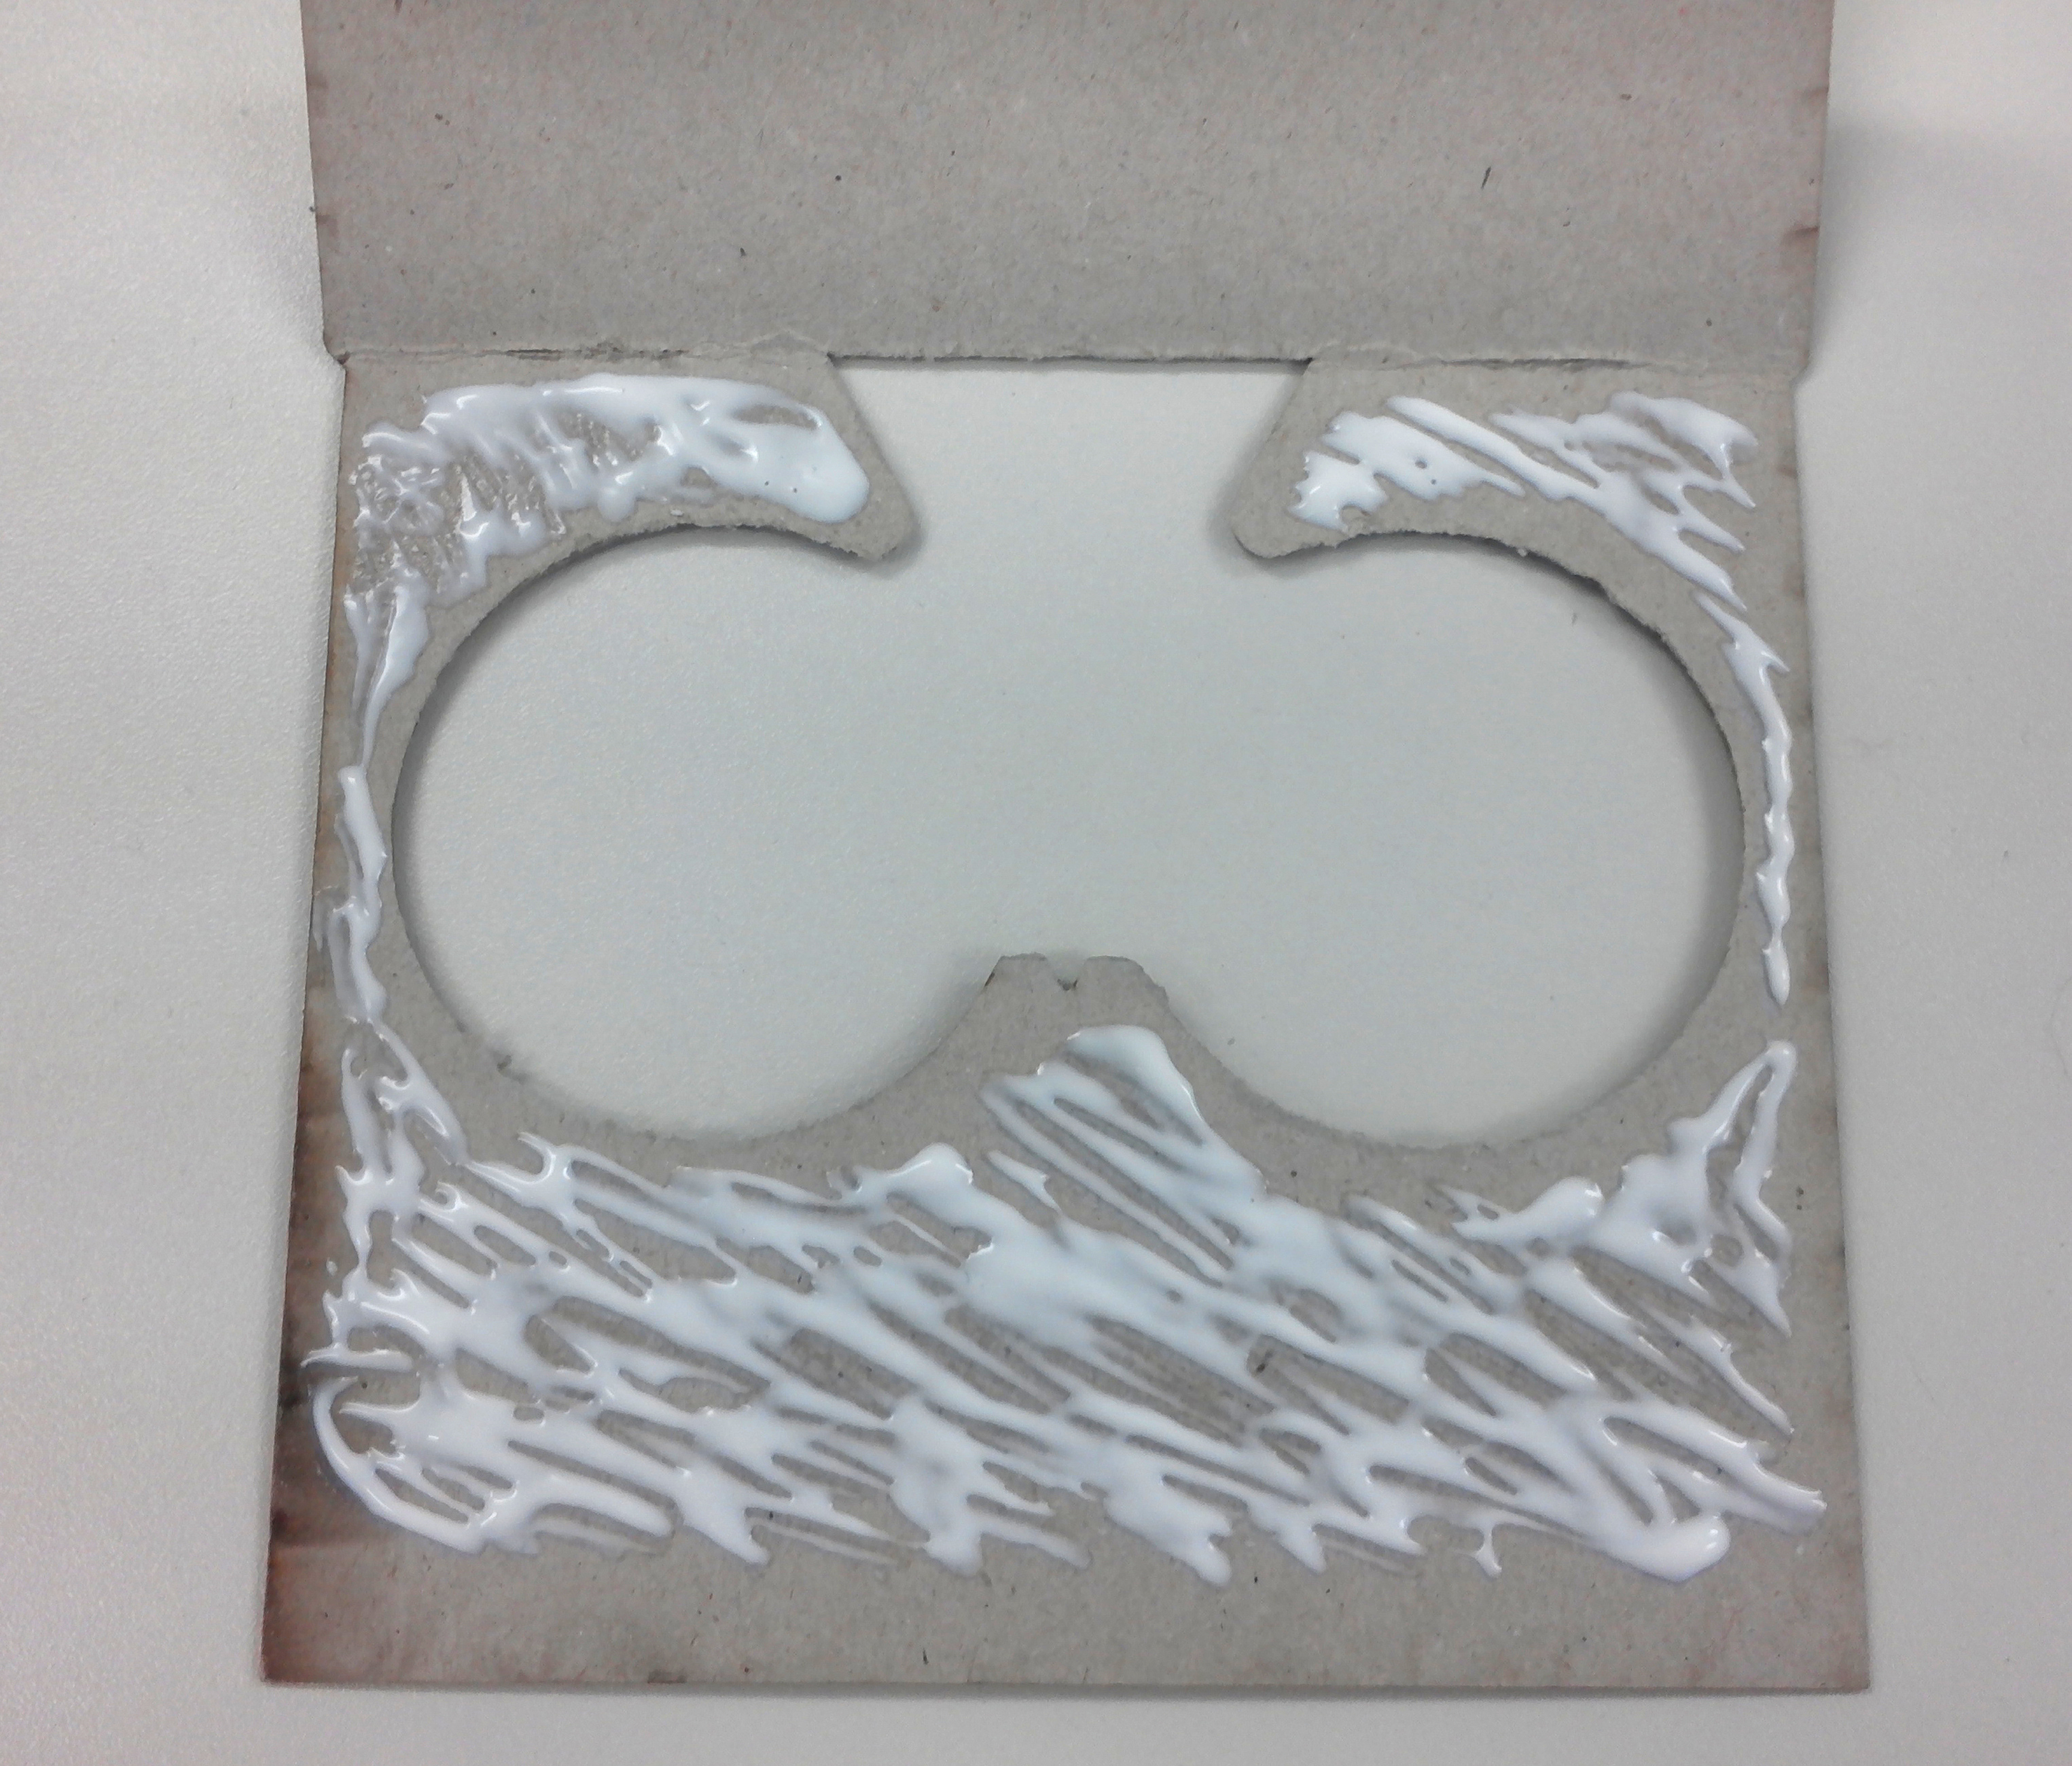
\includegraphics[width=0.42\linewidth]{partACD02}
		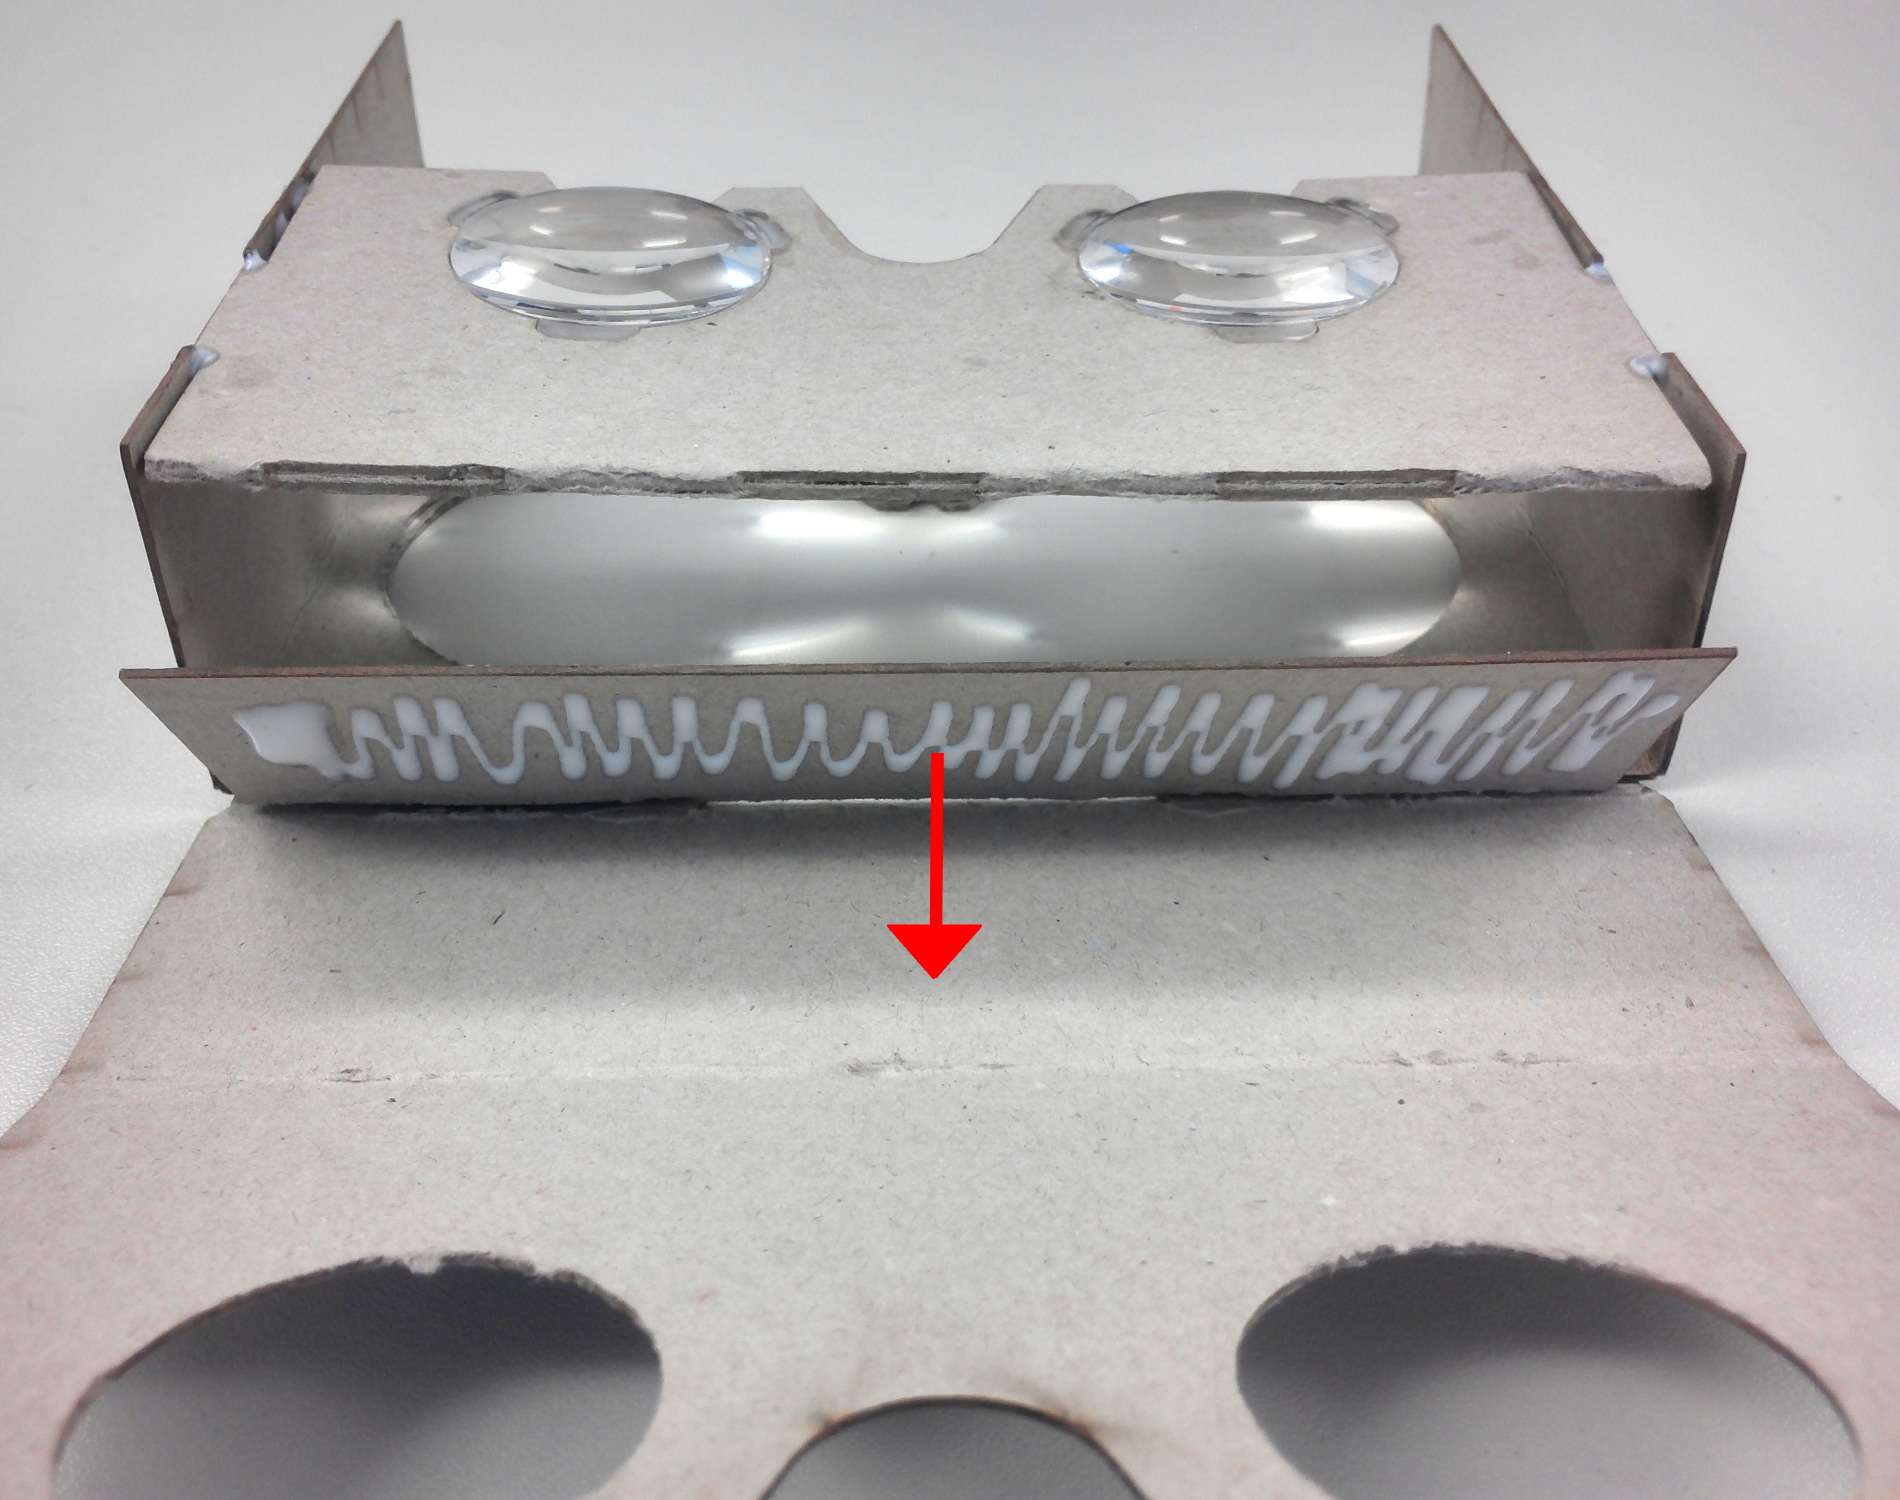
\includegraphics[width=0.45\linewidth]{partACD03} \\ \vspace{2mm}
		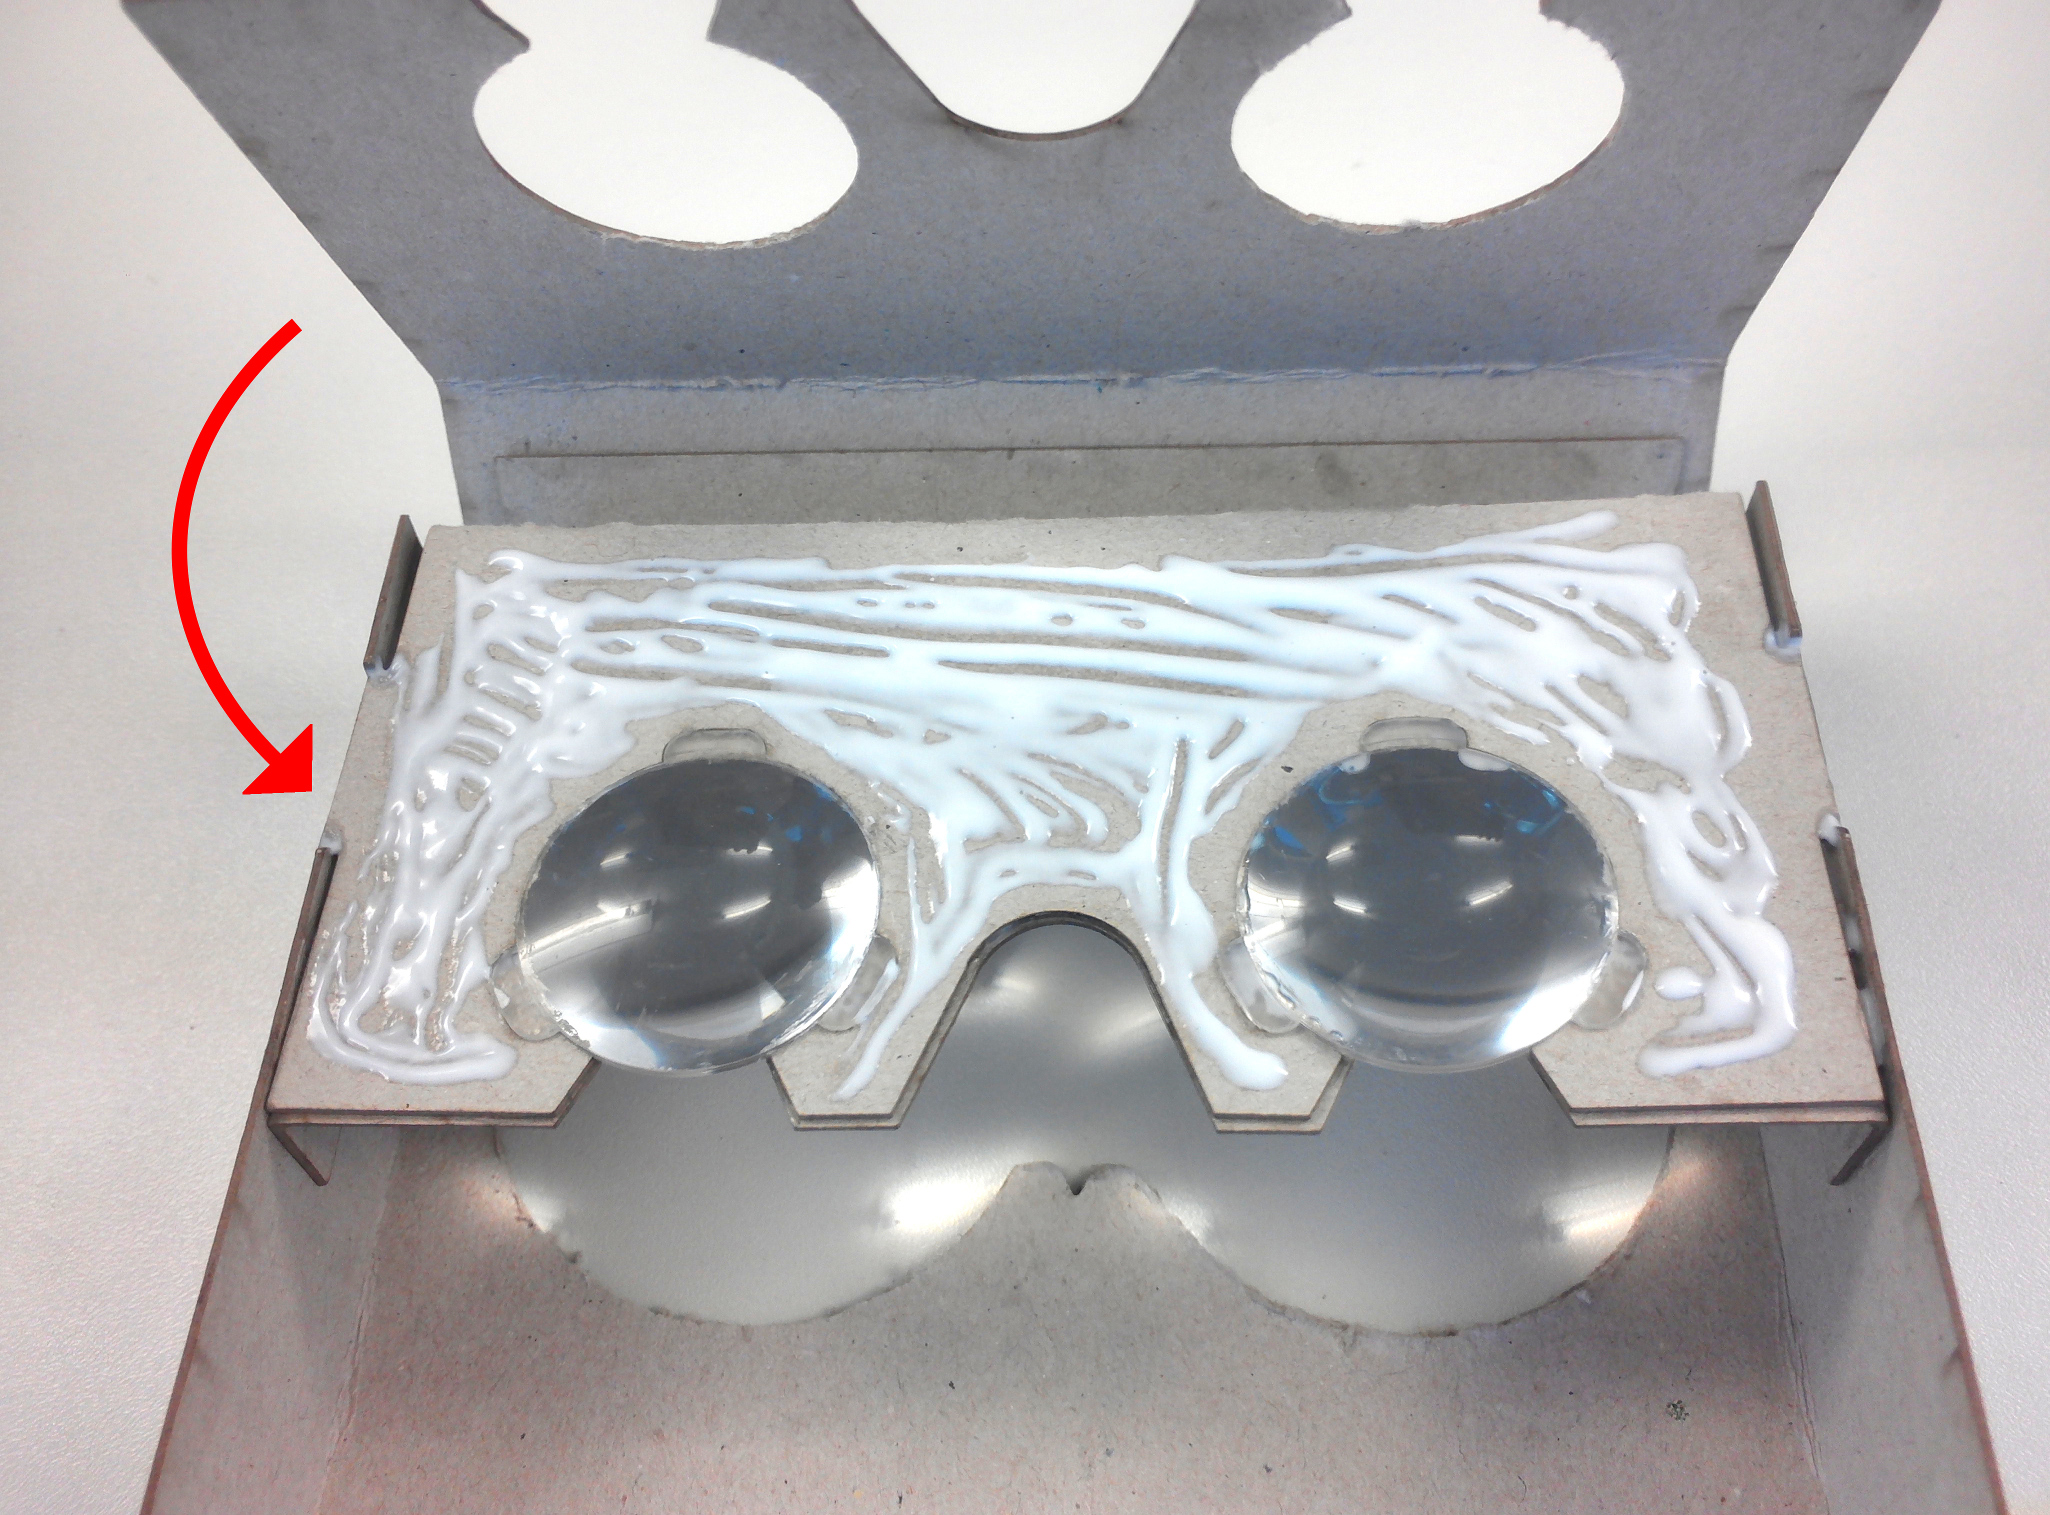
\includegraphics[width=0.45\linewidth]{partACD04}
		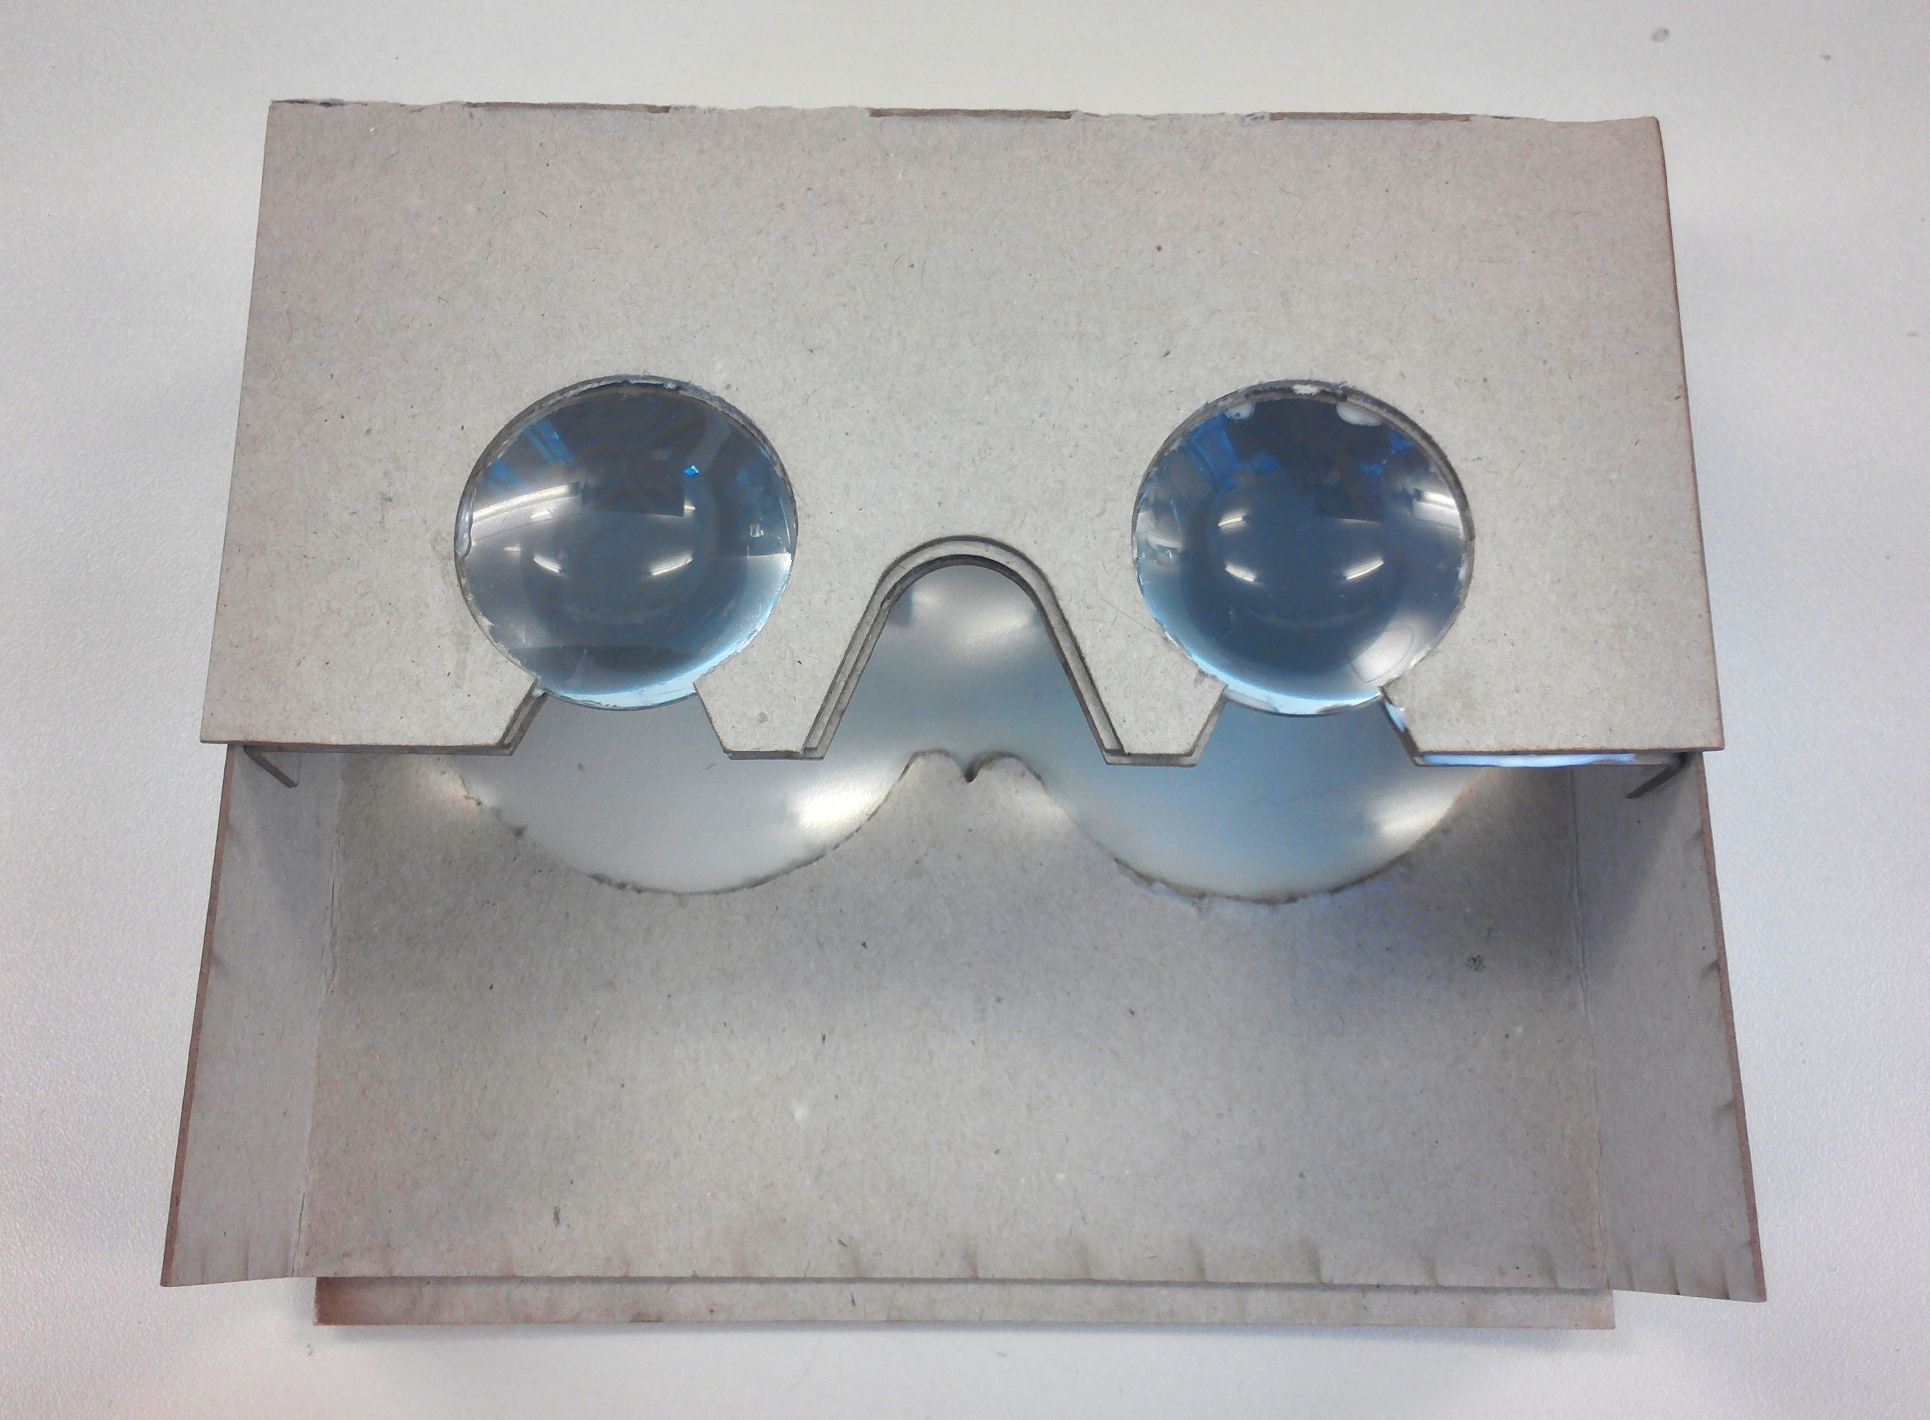
\includegraphics[width=0.45\linewidth]{partACD05}
		\caption{Positioning and Glueing of the A/C combination on part D}
		\label{fig:screenshot016}
	\end{figure}
	\clearpage
	\item Fold the edges of part E (see figure \ref{fig:screenshot017}). Make sure to fold the edges to the bottom-side of part E, a ``T'' marks the top-side of part E. This is important because the hole for the smartphone camera must be on the correct side. Place the part created in the previous step on part E (bottom-side) and glue it (figure \ref{fig:screenshot018}). Then glue the sides as well as the lid (Figures \ref{fig:screenshot018}, \ref{fig:screenshot019} and \ref{fig:screenshot020}).
	\begin{figure}[htb]
		\centering
		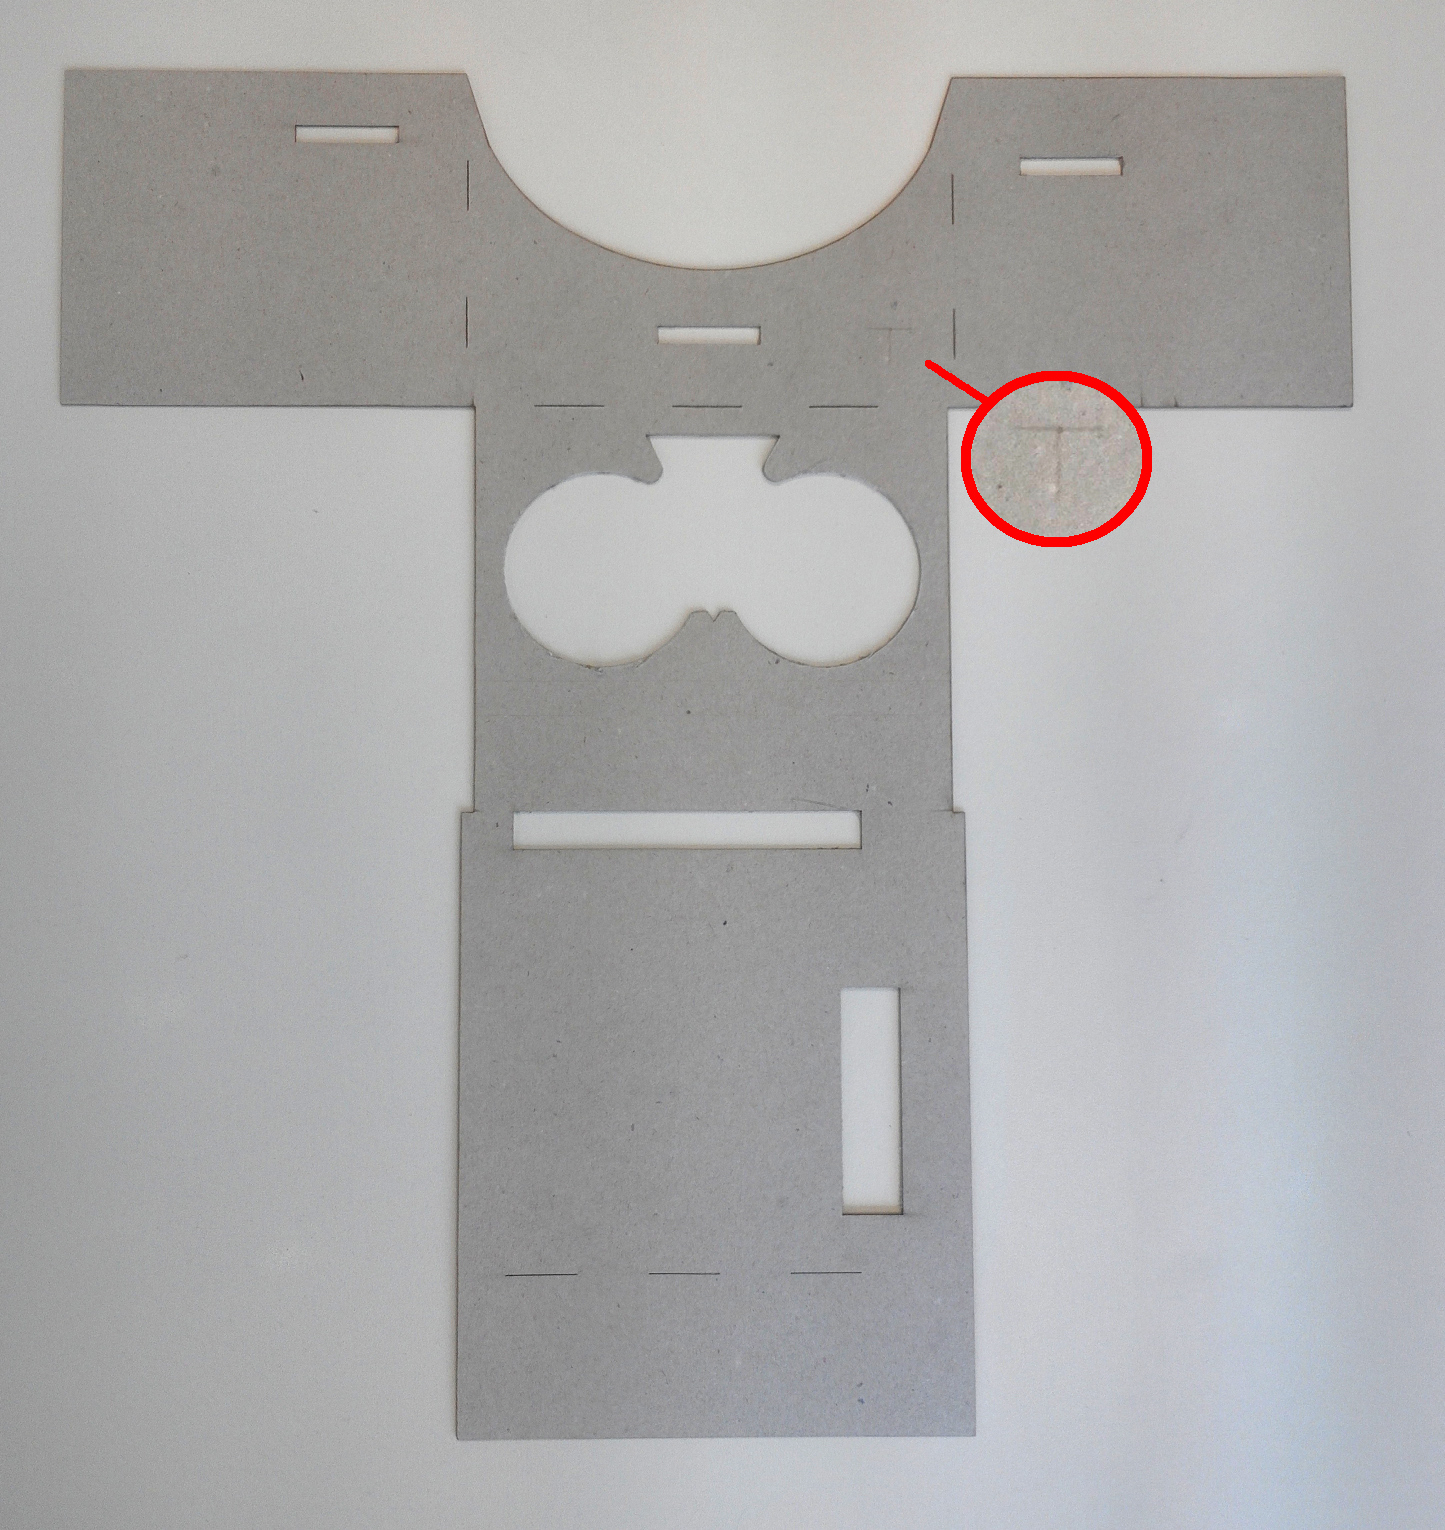
\includegraphics[width=0.75\linewidth]{partE01}
		\caption{Part E}
		\label{fig:screenshot017}
	\end{figure}
	\begin{figure}[htb]
		\centering
		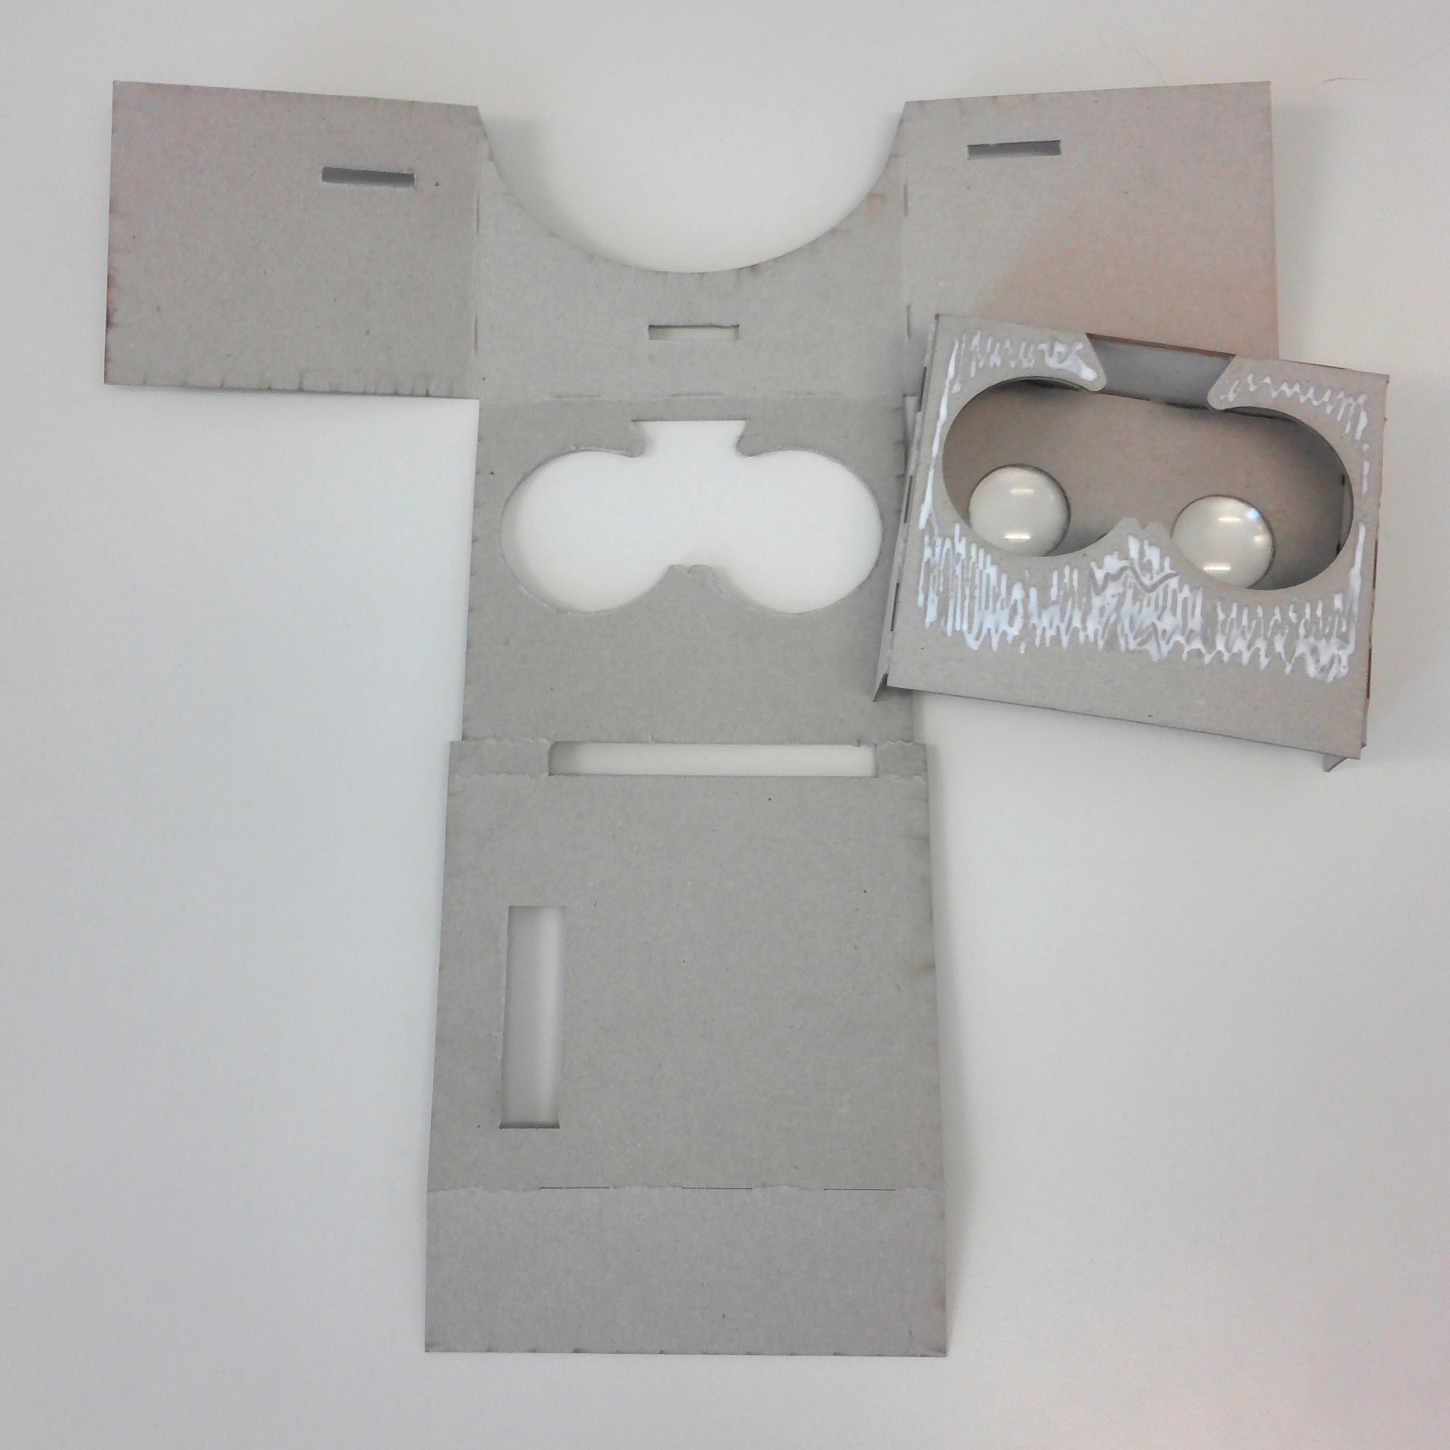
\includegraphics[width=0.475\linewidth]{partE02}
		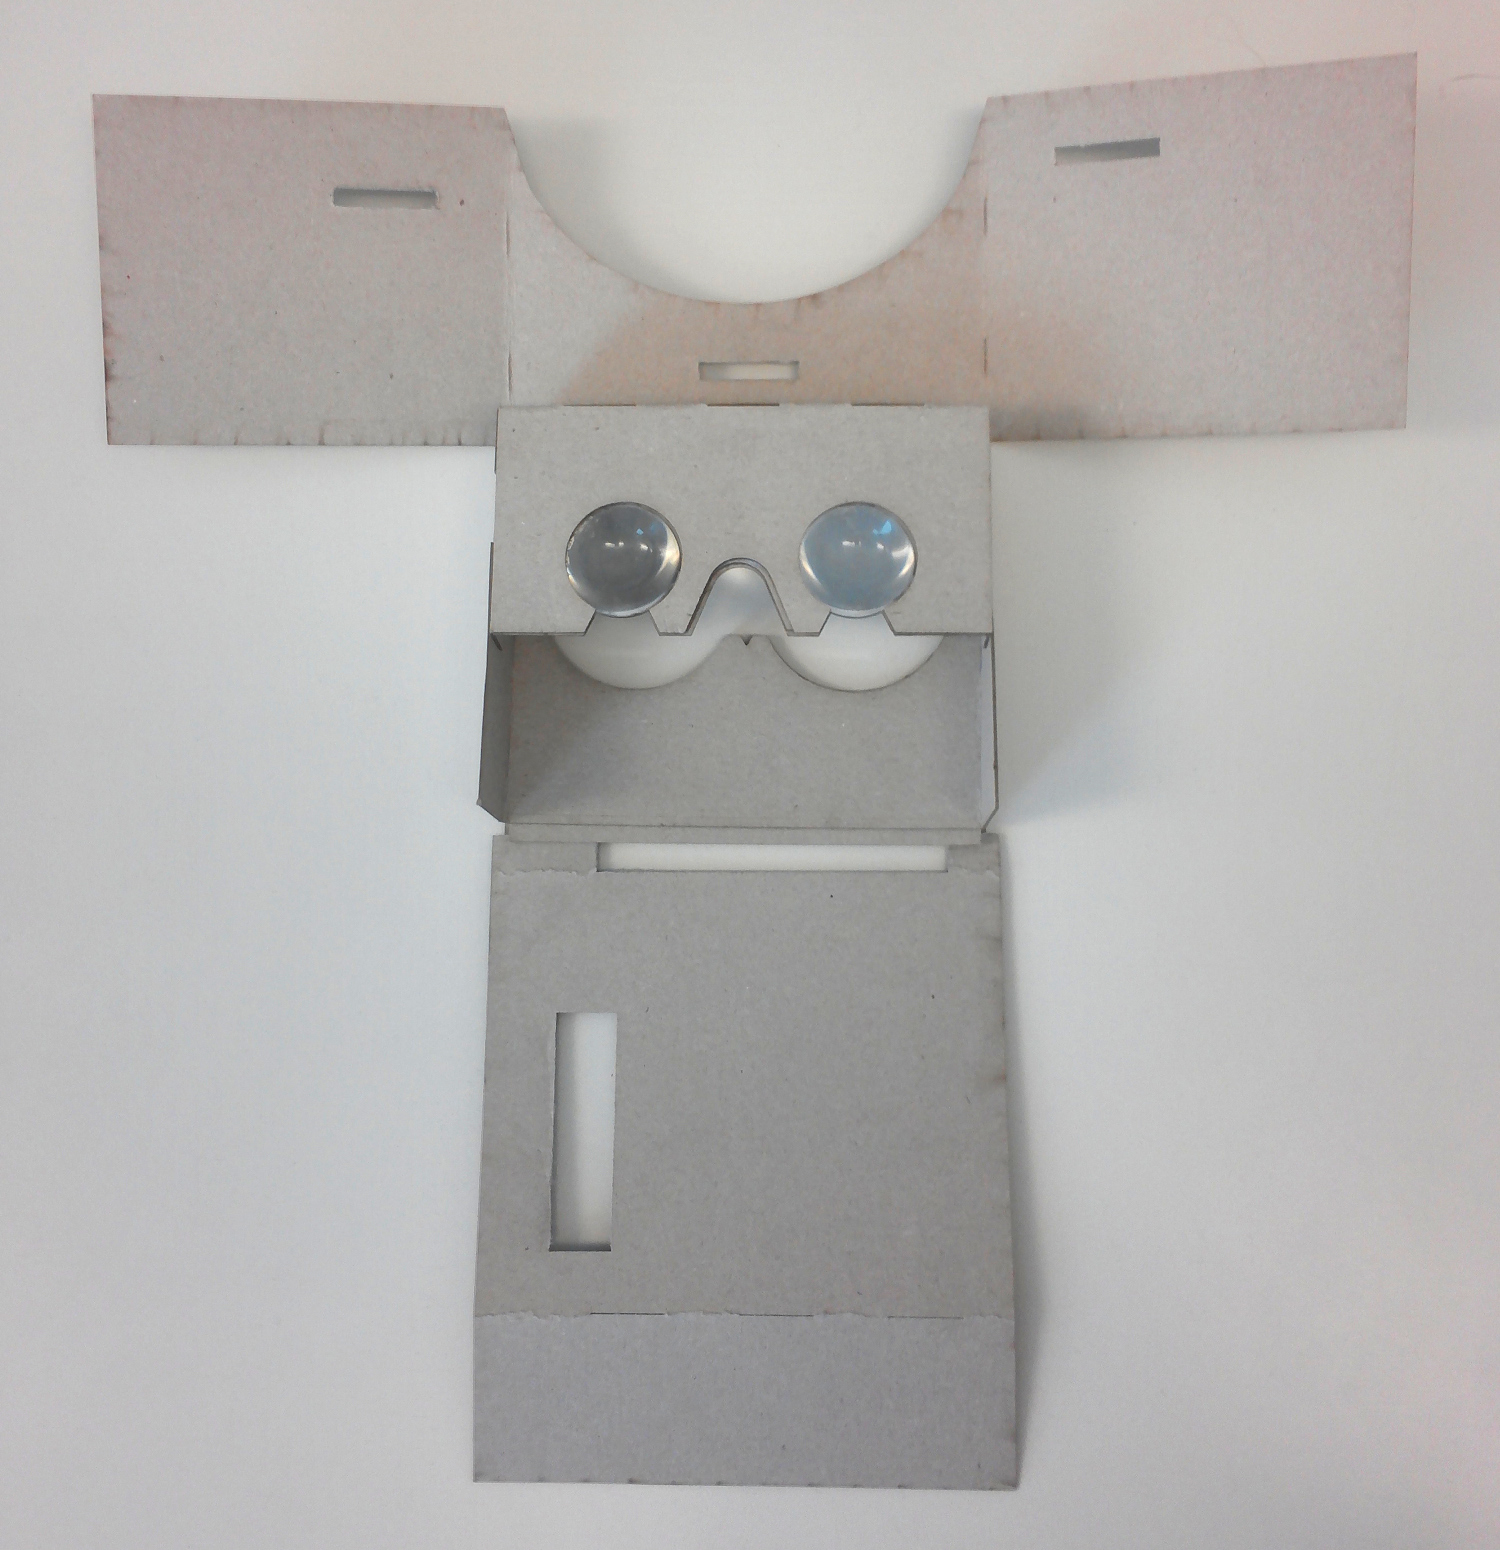
\includegraphics[width=0.46\linewidth]{partE03}
		\caption{Combination of both parts}
		\label{fig:screenshot018}
	\end{figure}
	\begin{figure}[htb]
	\centering
		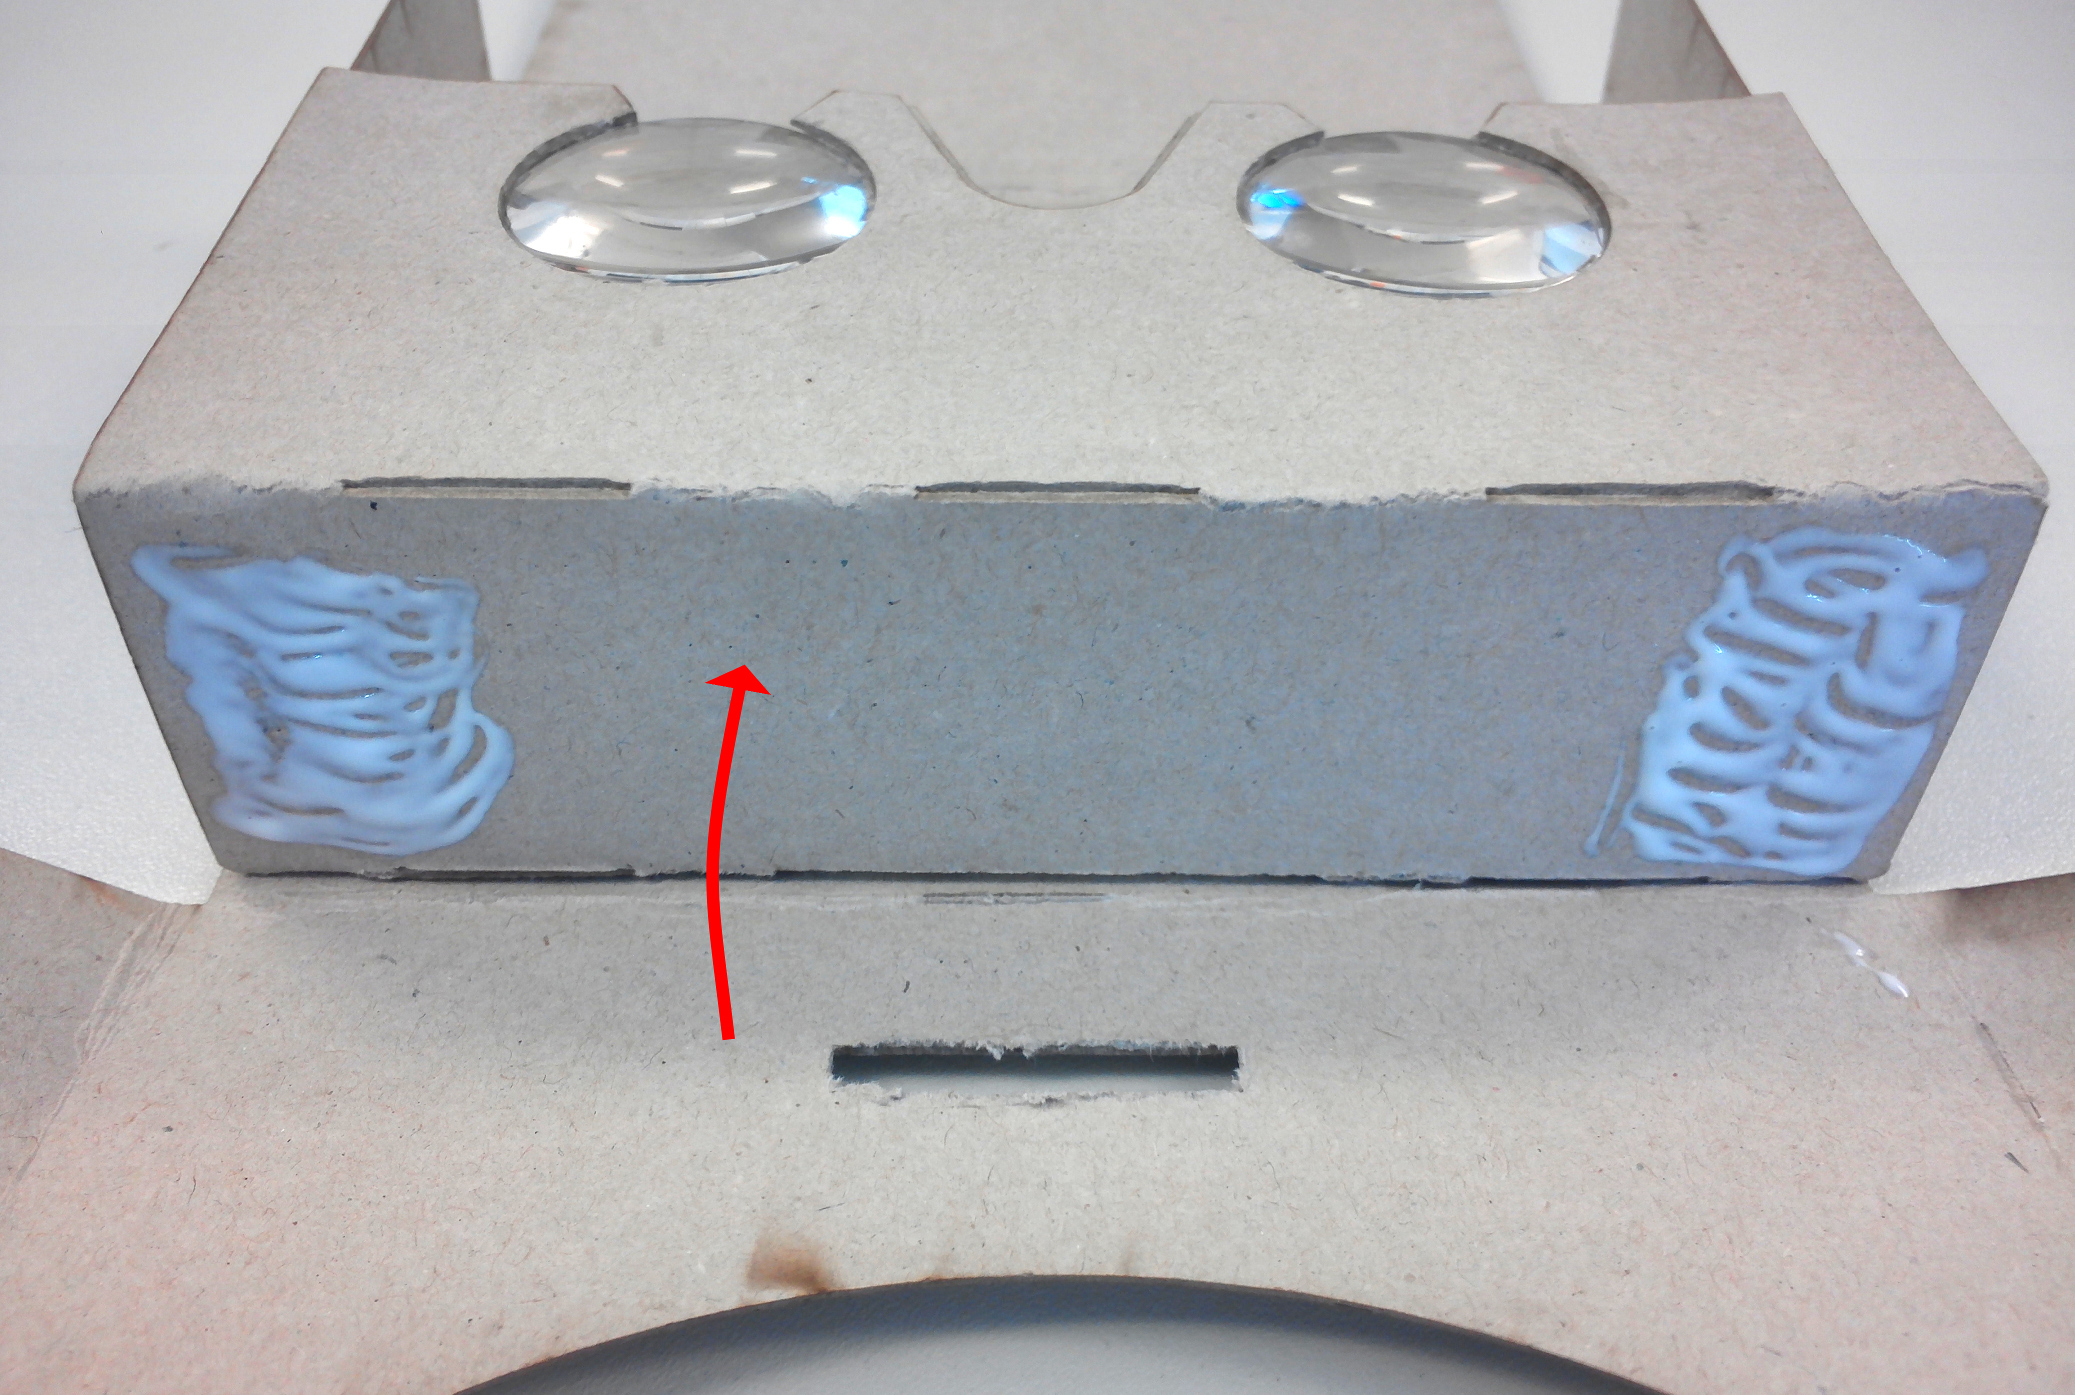
\includegraphics[width=0.7\linewidth]{partE04}
		\caption{Glueing the top of the cardboard}
		\label{fig:screenshot019}
	\end{figure}	
	\begin{figure}[htb]
		\centering
		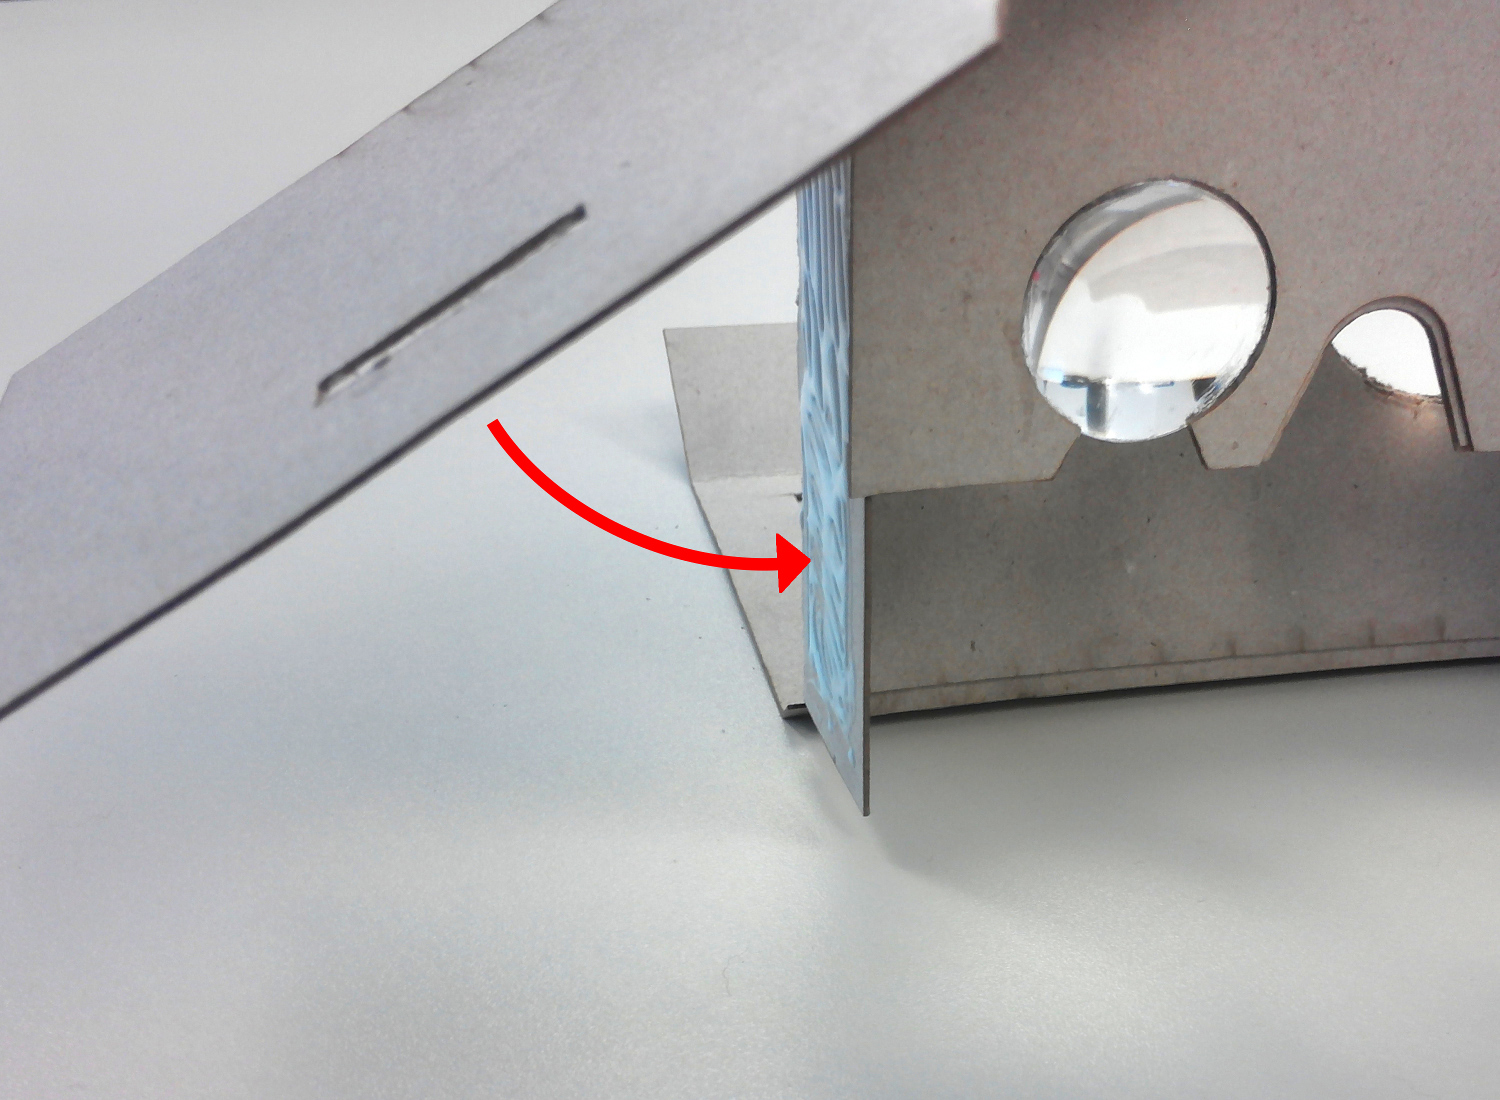
\includegraphics[width=0.6\linewidth]{partE05}\\ \vspace{2mm}
		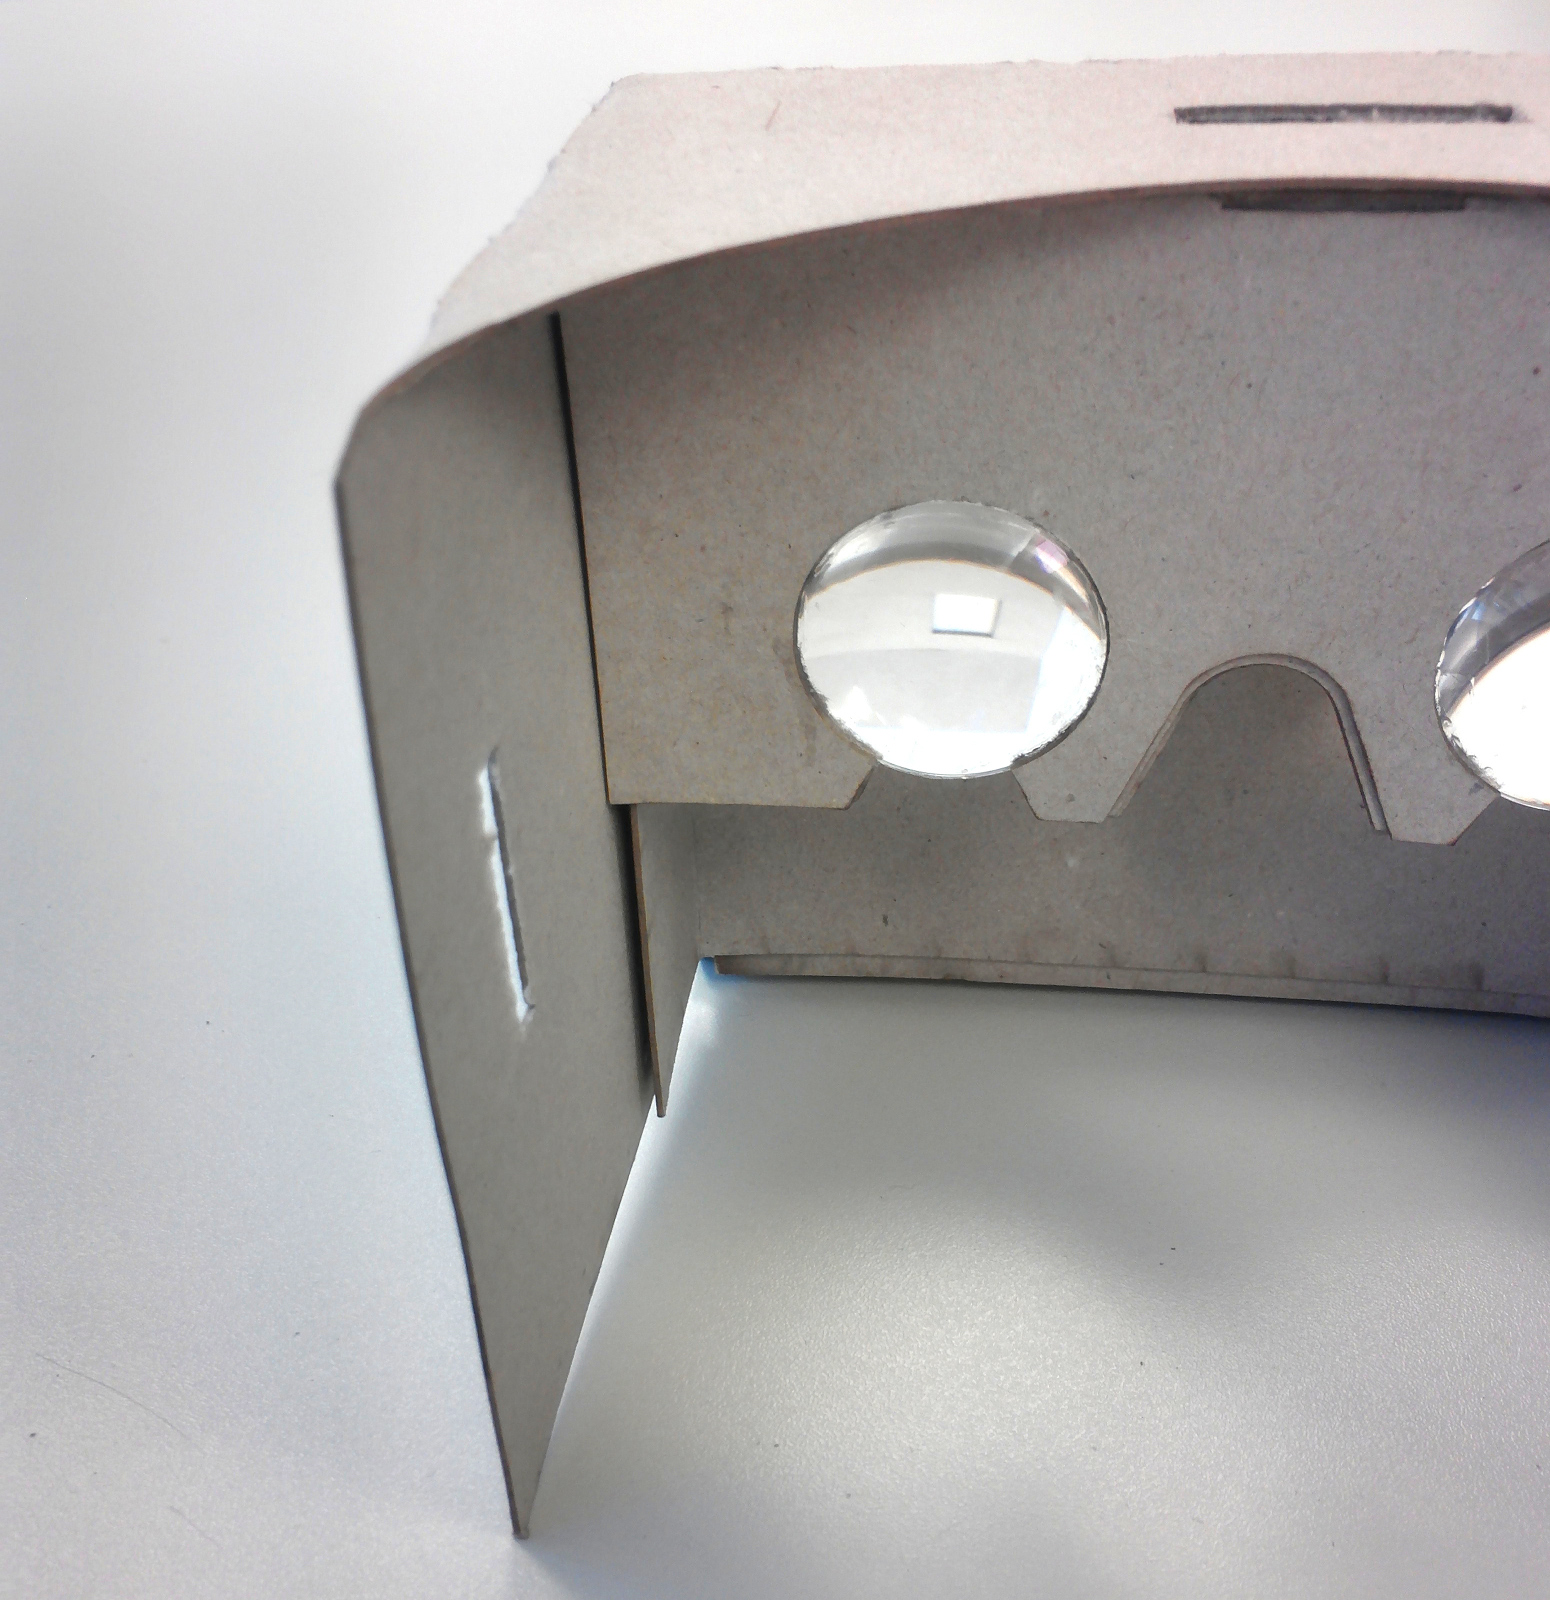
\includegraphics[width=0.6\linewidth]{partE06}
		\caption{Positioning of the cardboard sides}
		\label{fig:screenshot020}
	\end{figure}
	\clearpage
	\item Glue the six equal parts of F on top of each other (Figure \ref{fig:screenshot021}) and glue them between the engraved lines onto the cardboard (see figure \ref{fig:screenshot022}).
	\begin{figure}[htb]
		\centering
		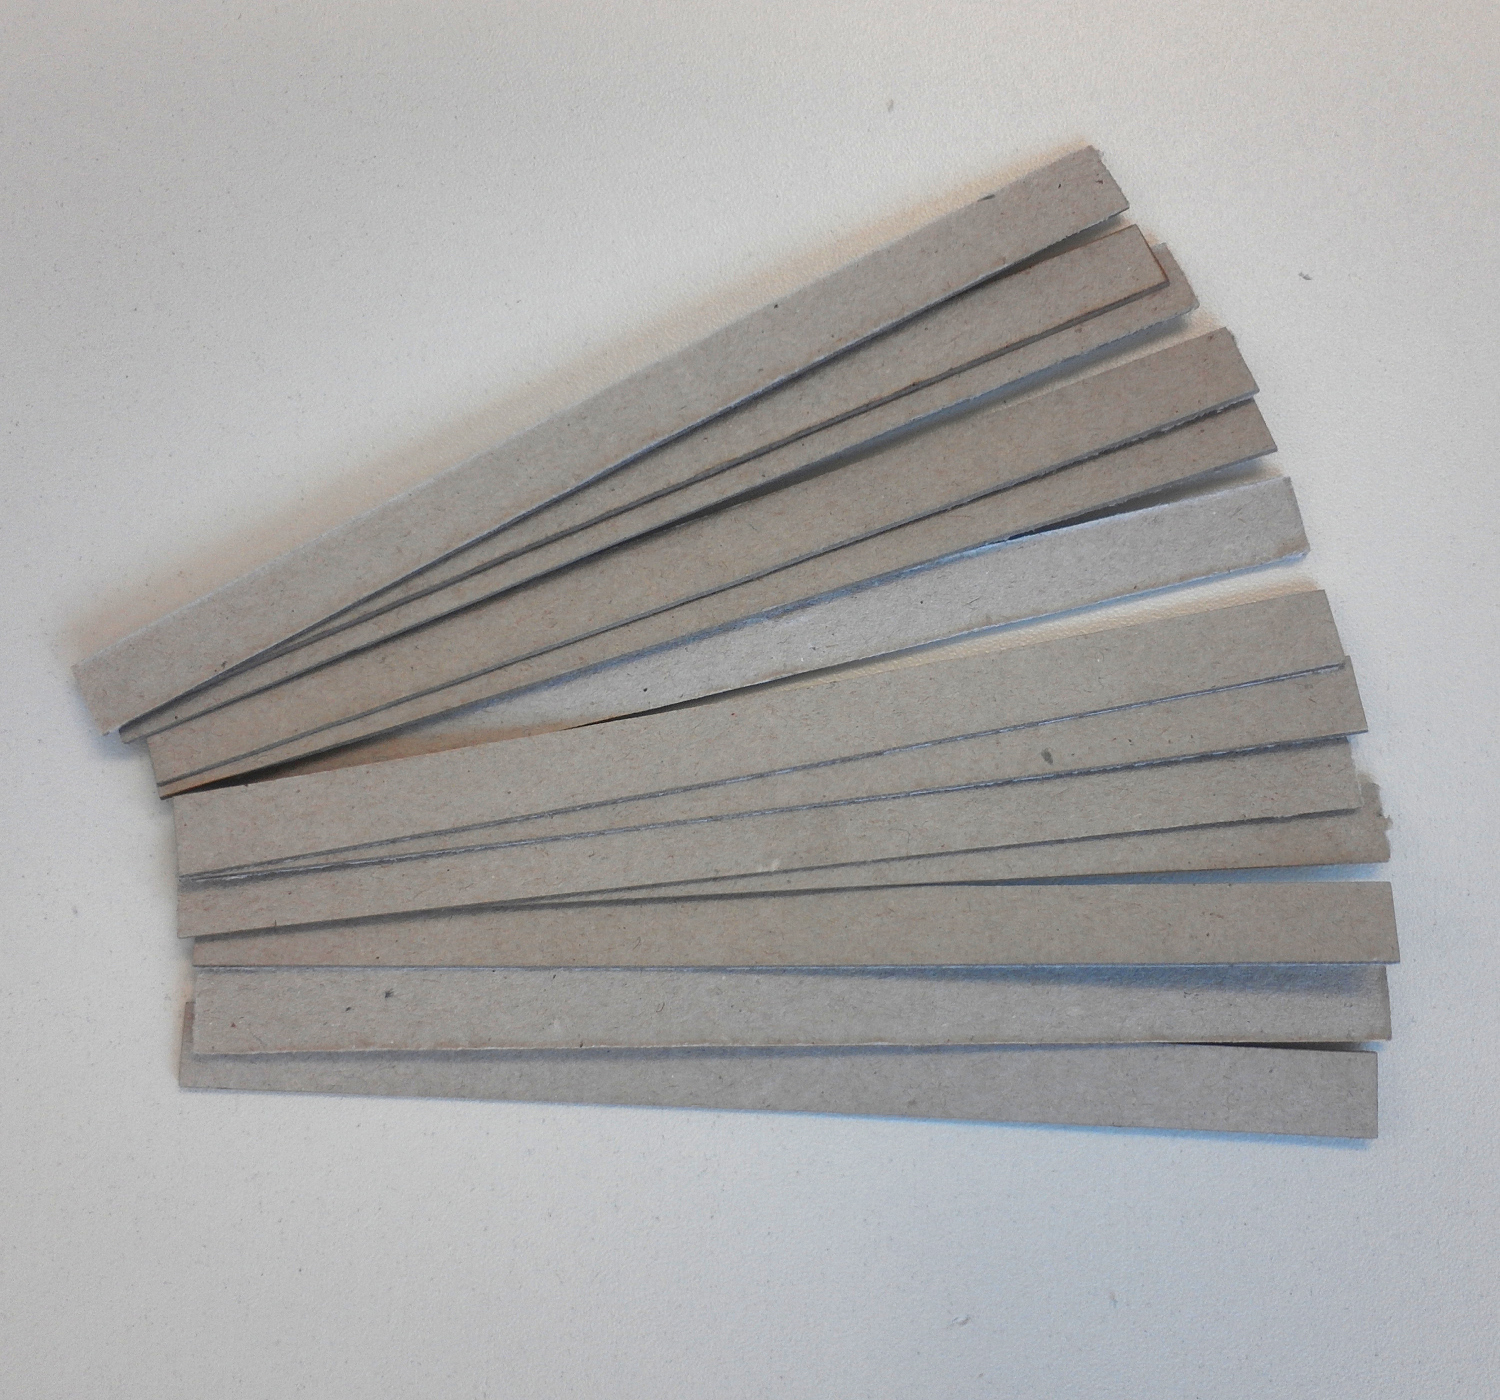
\includegraphics[width=0.45\linewidth]{partF01}
		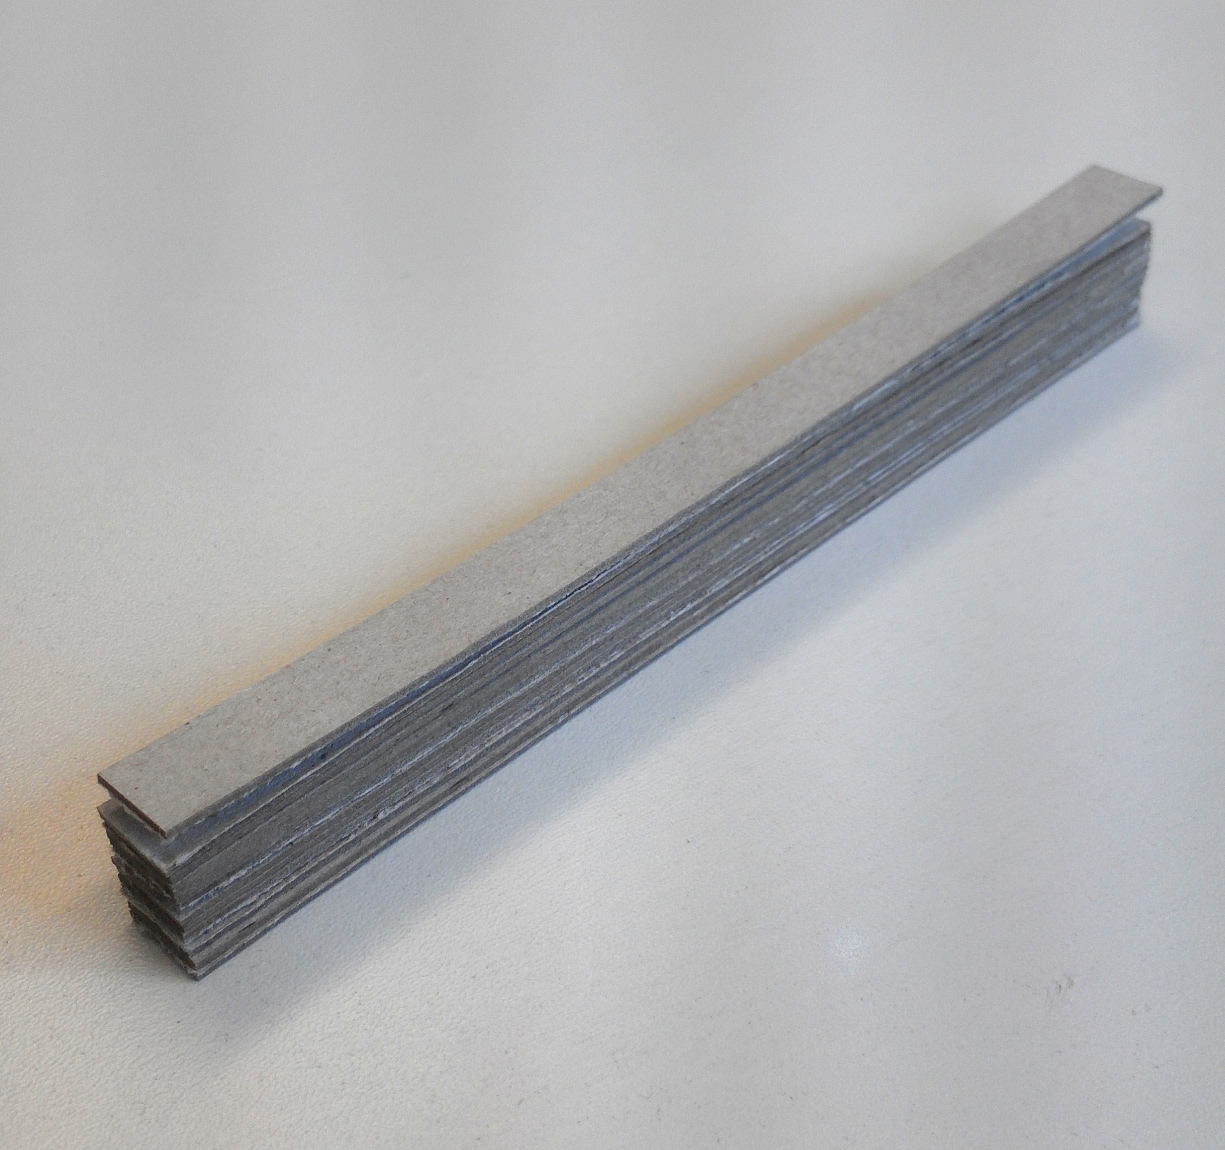
\includegraphics[width=0.45\linewidth]{partF02}
		\caption{Assembling of part F}
		\label{fig:screenshot021}
	\end{figure}
	\begin{figure}[!htb]
		\centering
		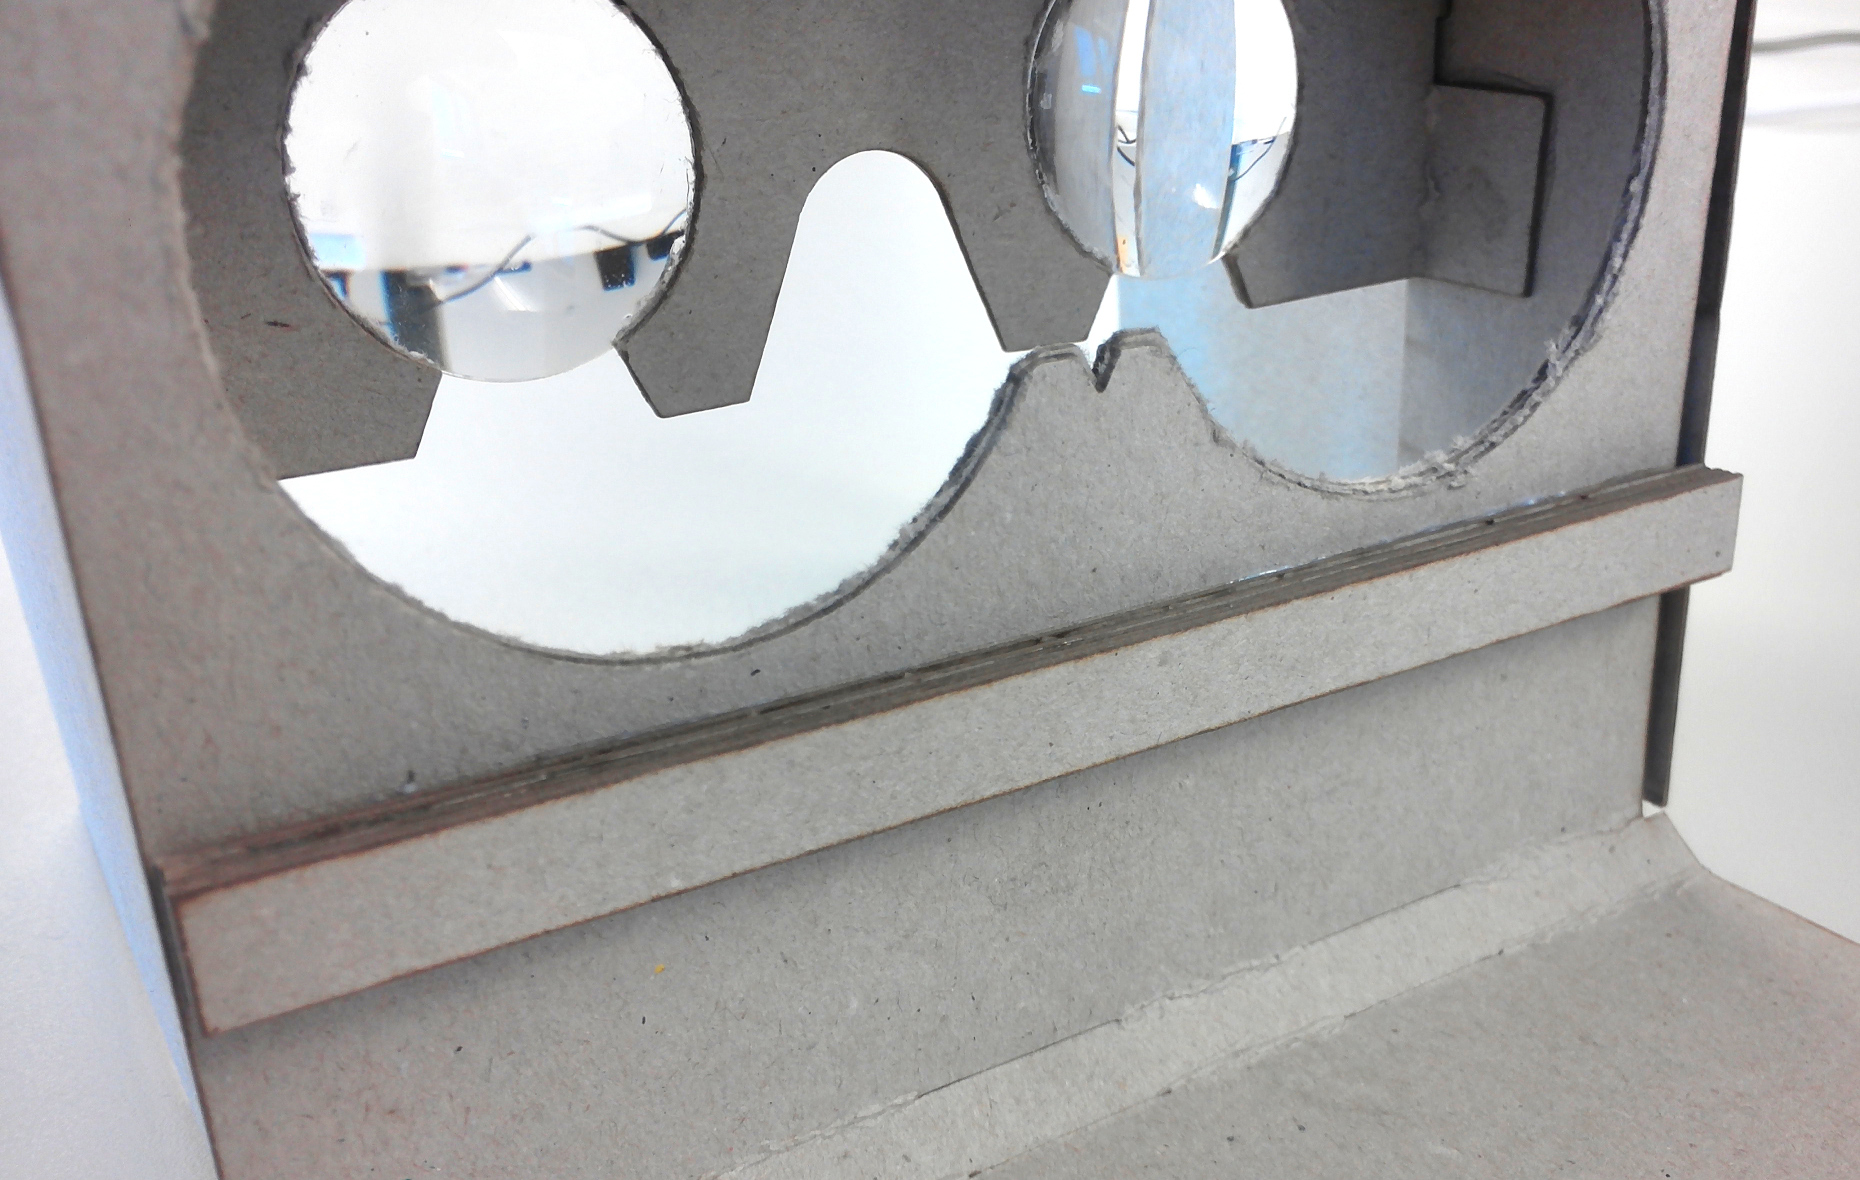
\includegraphics[width=0.75\linewidth]{partF03}
		\caption{Positioning part F onto the cardboard}
		\label{fig:screenshot022}
	\end{figure}
	\clearpage	
	
	\item For the next step take some foam rubber and cut out a stripe and a triangle, like the ones shown in figure \ref{fig:foamrubber1}. Then glue them to the inside of the cardboard: Attach the stripe into the gap between the lenses and the triangle on the area above it. The result should look like on figure \ref{fig:foamrubber2}.
	\begin{figure}[!htb]
		\centering
		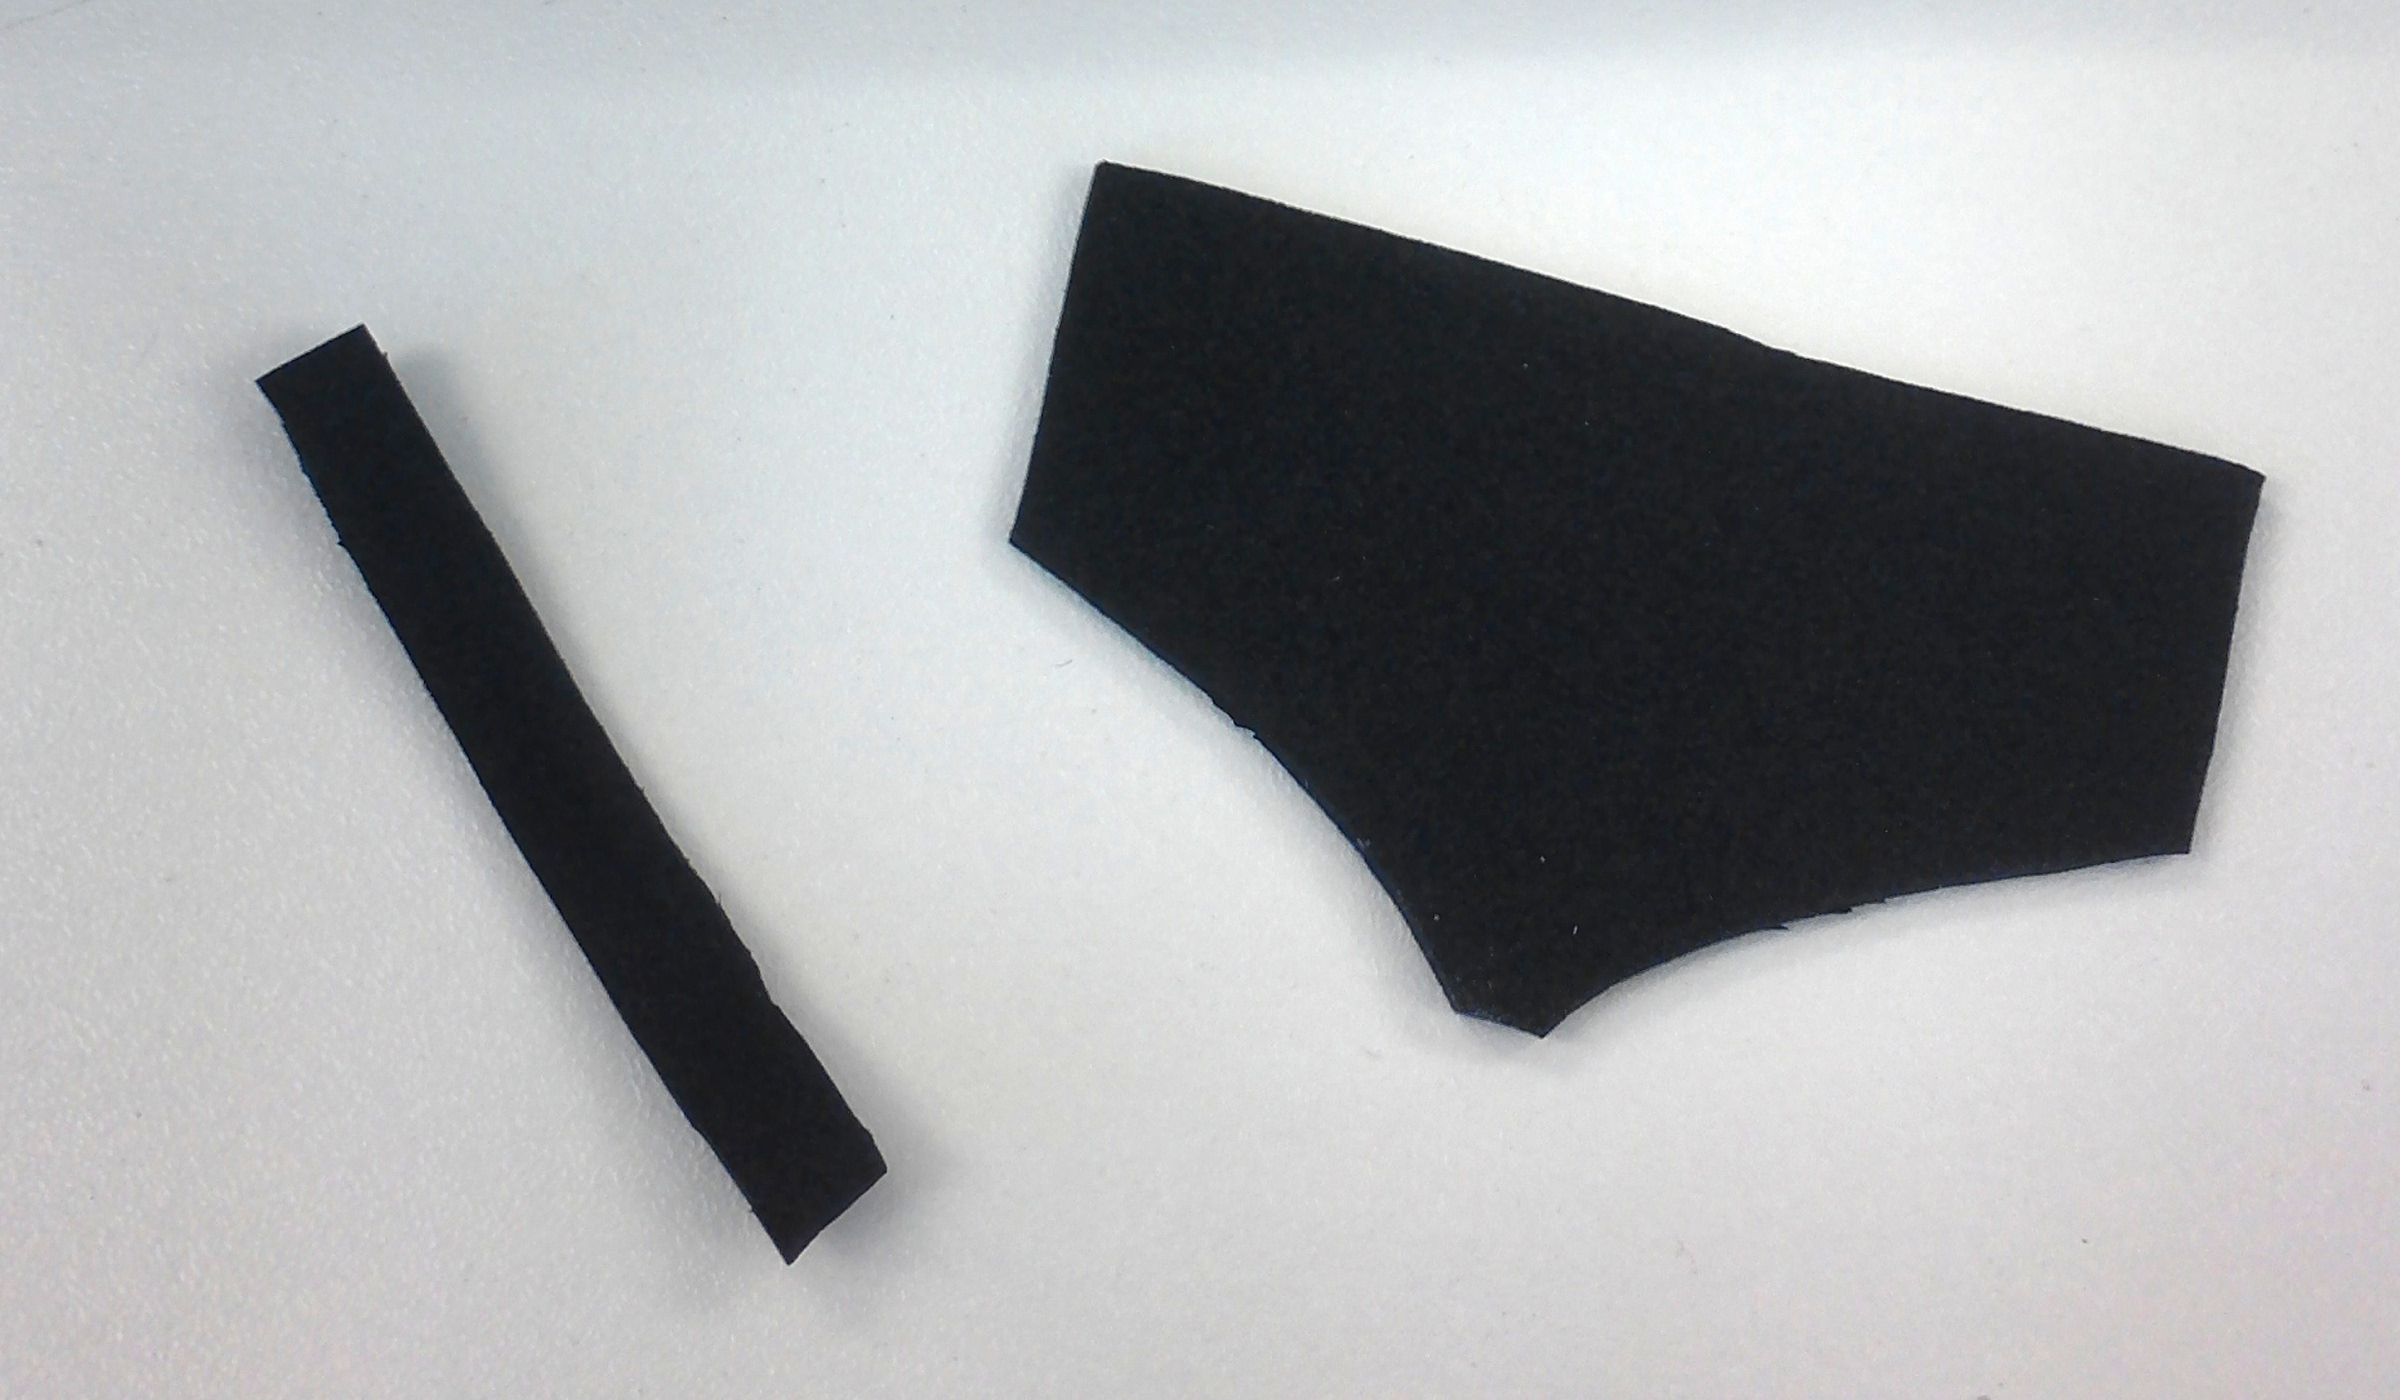
\includegraphics[width=0.75\linewidth]{foamrubber01}
		\caption{cut foam rubber as padding for the inside of the cardboard}
		\label{fig:foamrubber1}
	\end{figure}
	\begin{figure}[!htb]
		\centering
		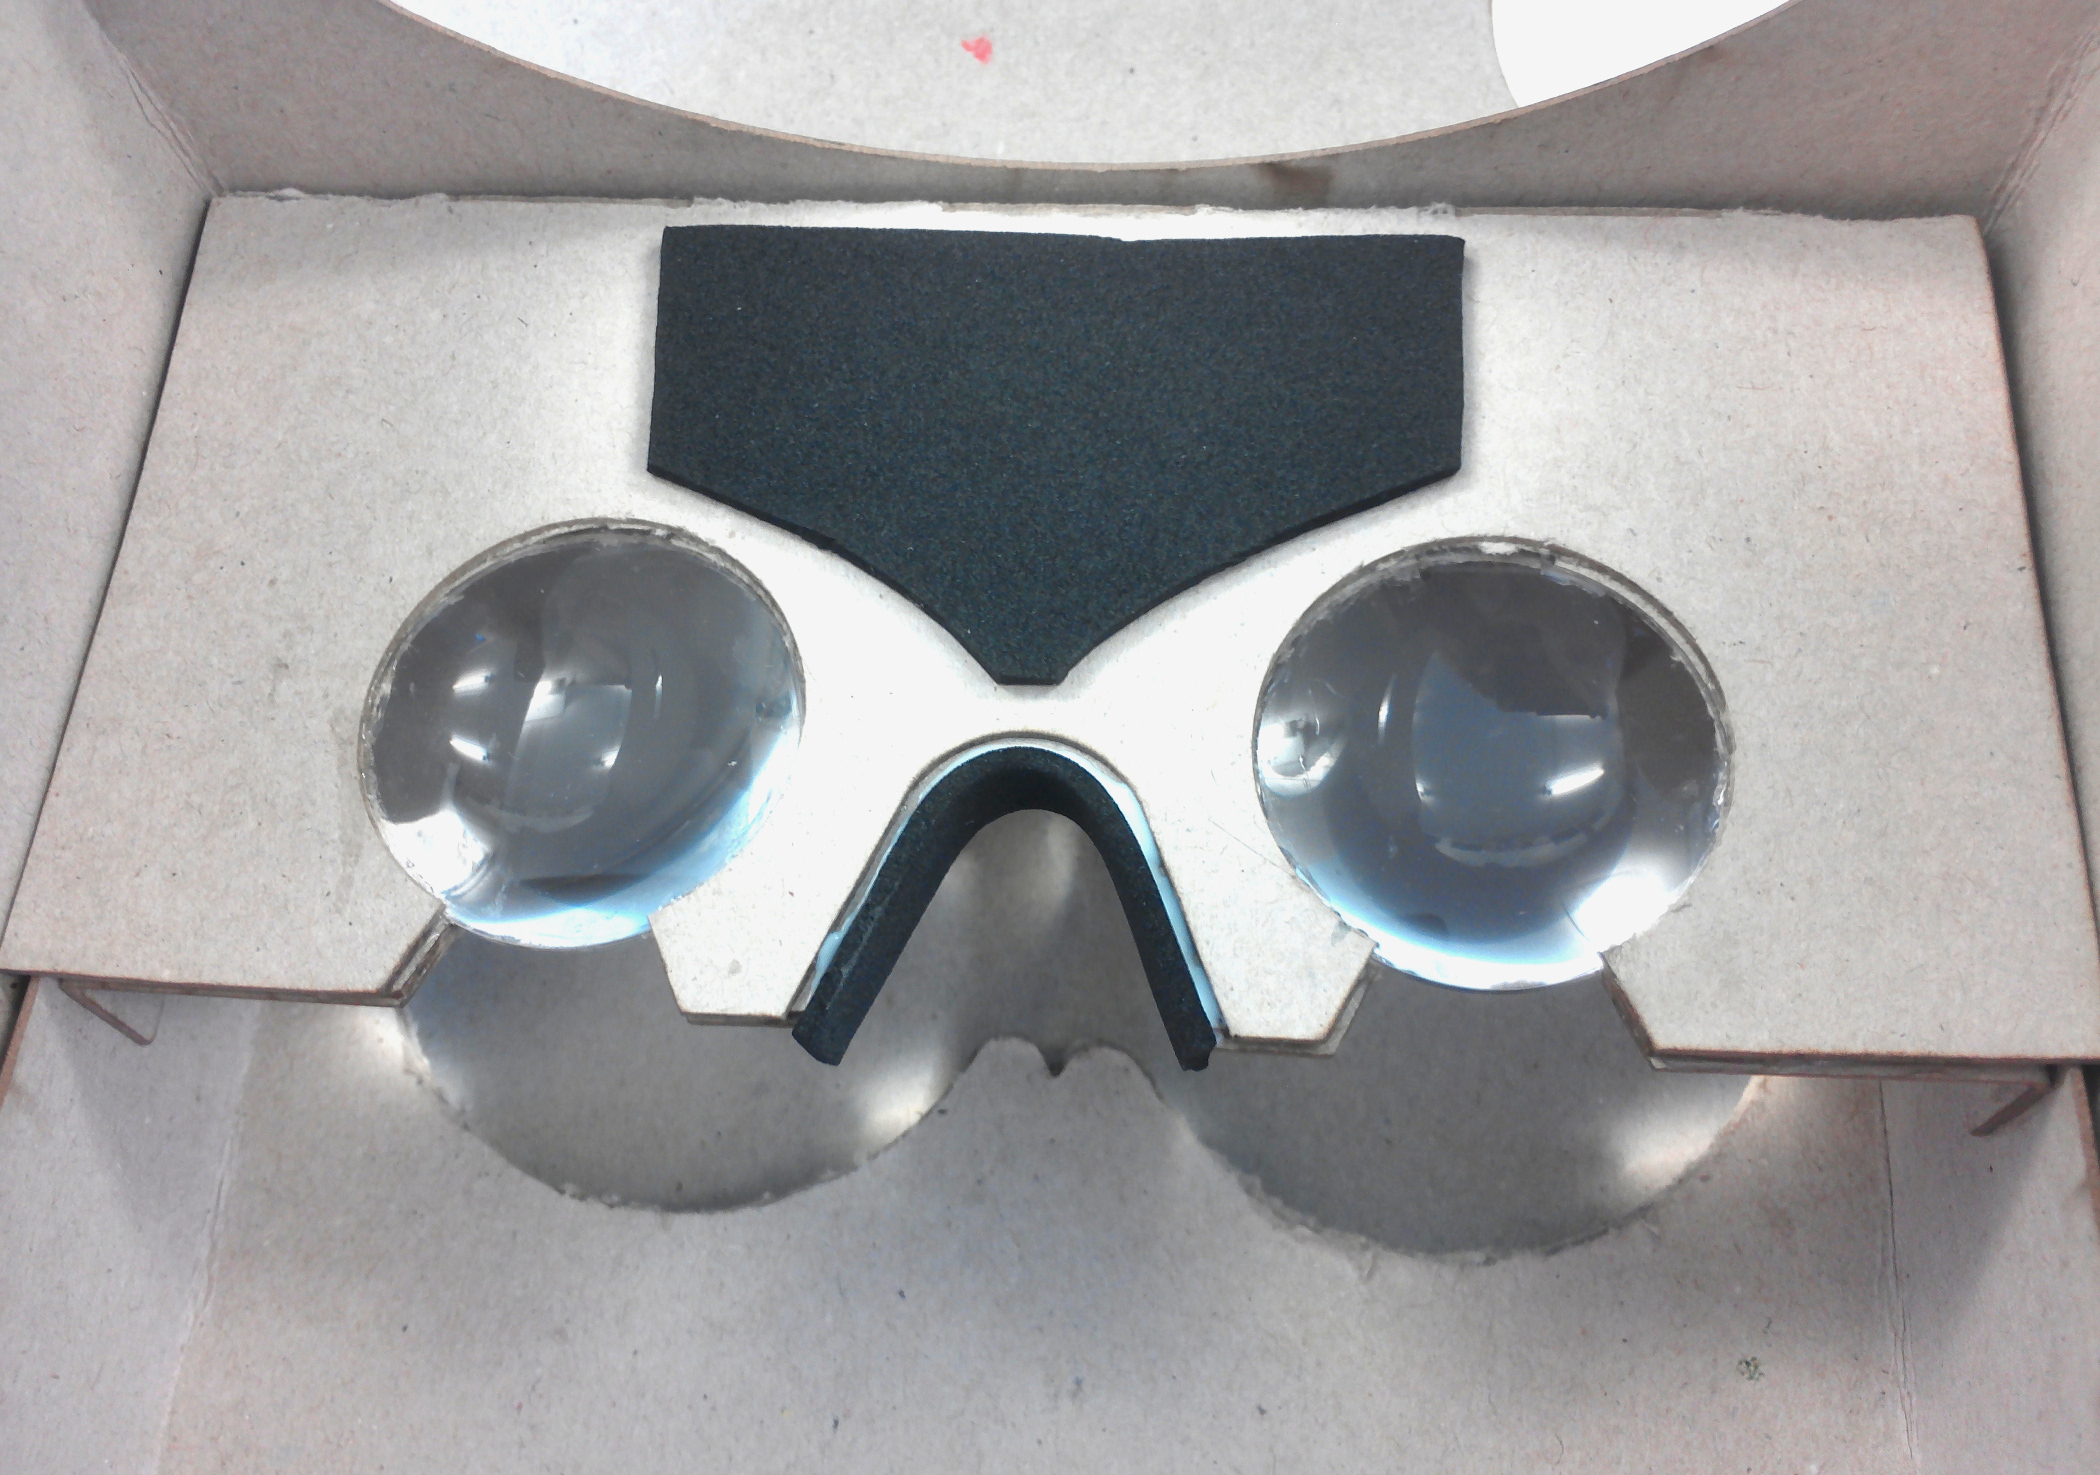
\includegraphics[width=0.75\linewidth]{foamrubber02}
		\caption{foam rubber attached on the cardboard}
		\label{fig:foamrubber2}
	\end{figure}
	
	\item Next, take some more foam rubber and cut out a rectangle (see figure \ref{fig:holder1}). Glue this rectangle between the squarish apertures of part B as shown in figure \ref{fig:holder2}.
	\begin{figure}[!htb]
		\centering
		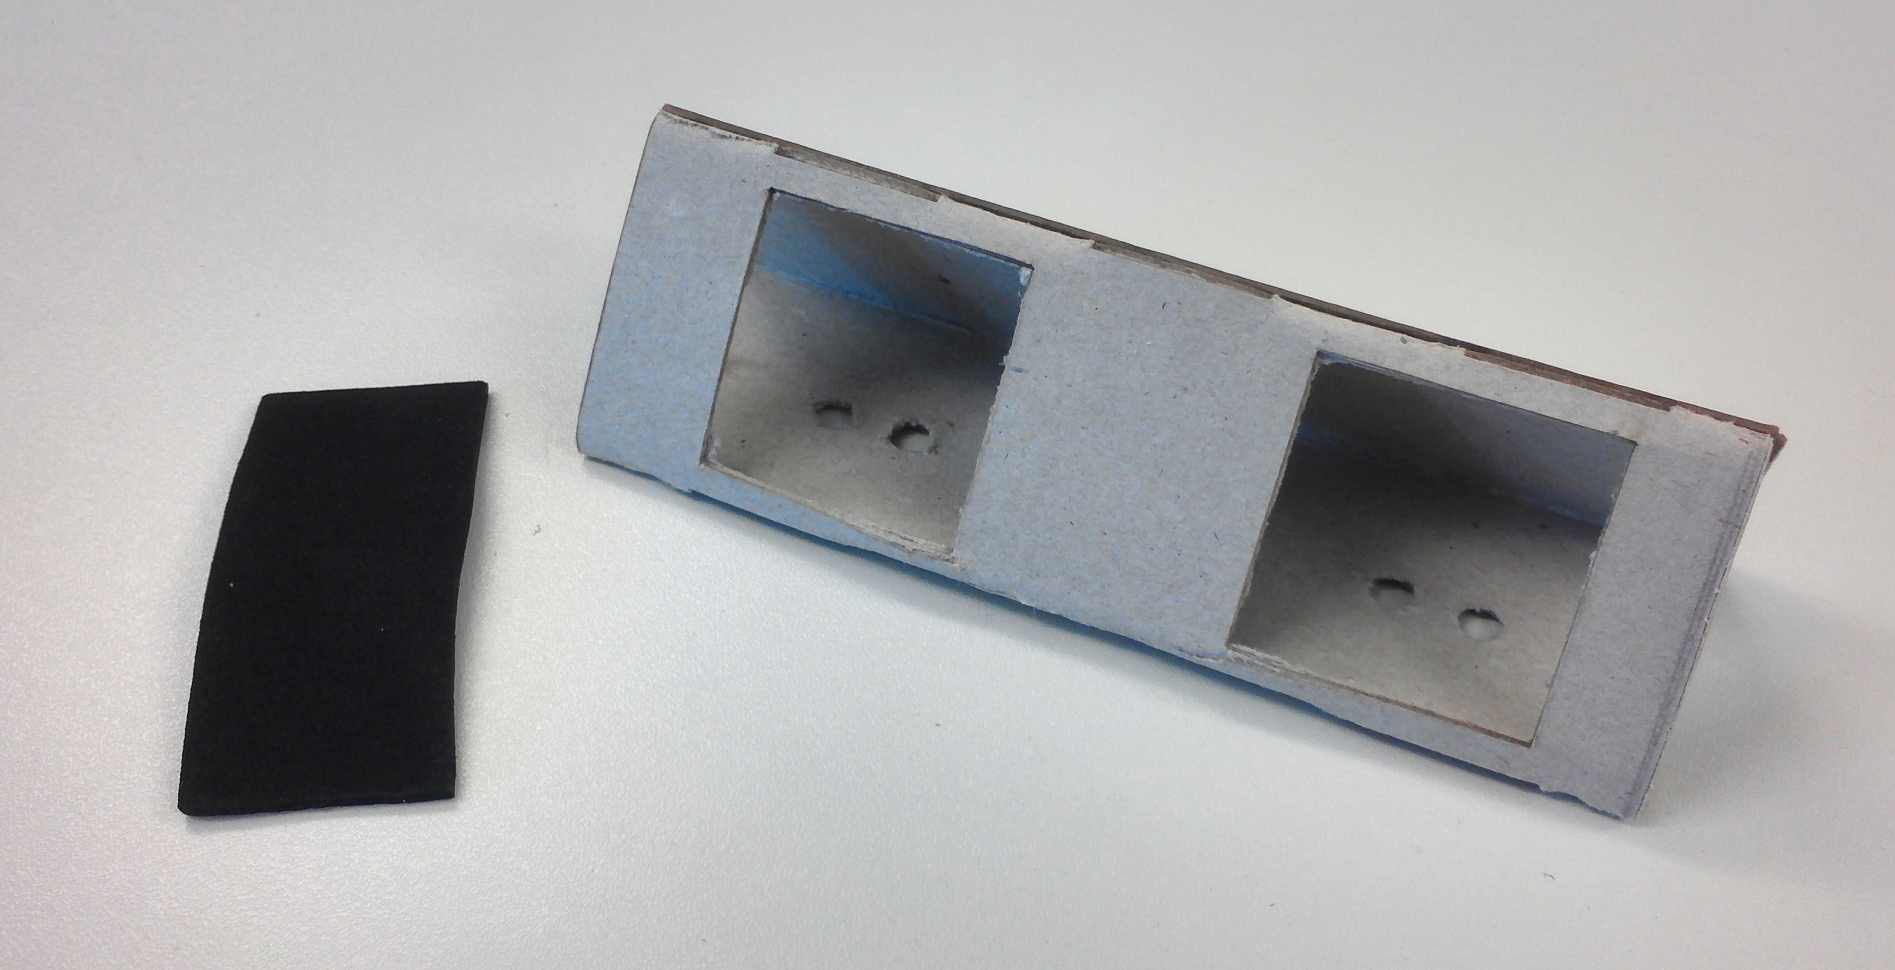
\includegraphics[width=0.75\linewidth]{holder01}
		\caption{cut foam rubber as padding for the inside of the cardboard}
		\label{fig:holder1}
	\end{figure}
	\begin{figure}[!htb]
		\centering
		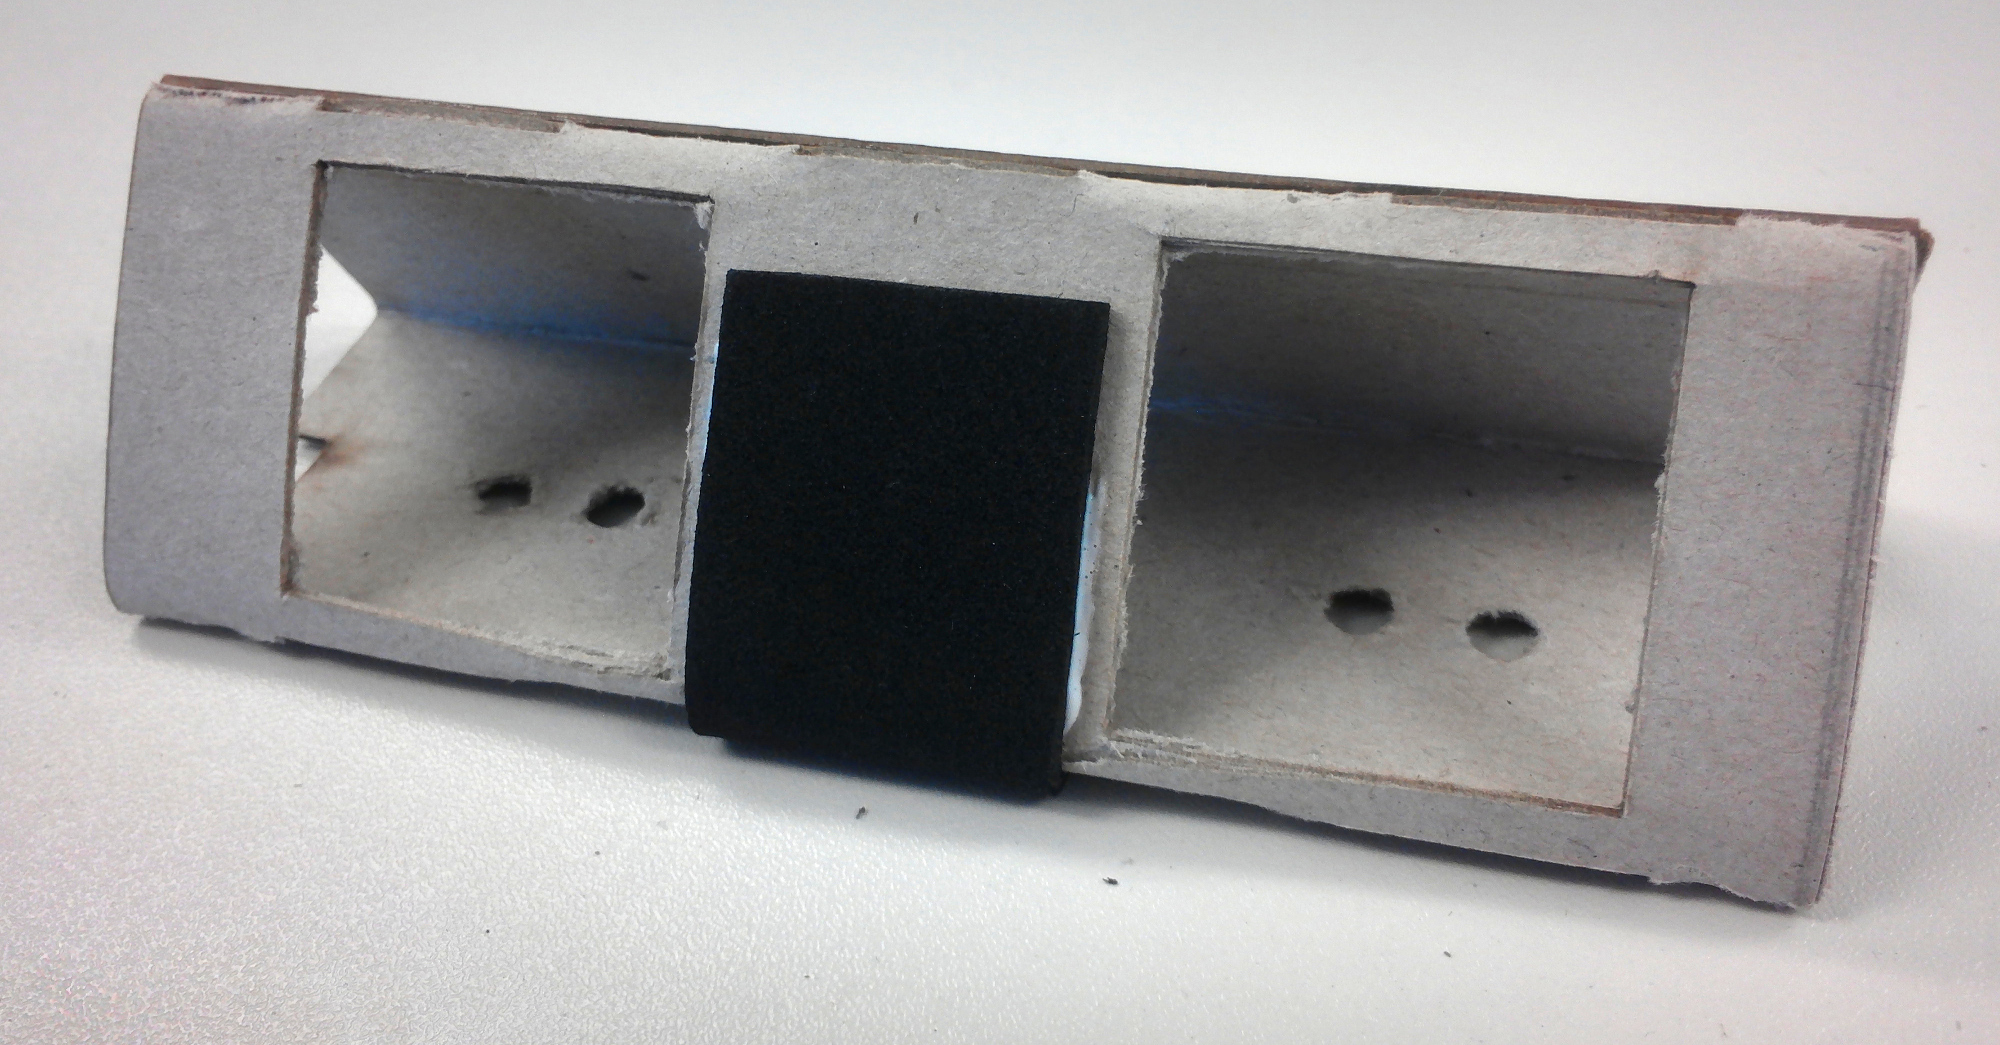
\includegraphics[width=0.75\linewidth]{holder02}
		\caption{foam rubber attached on the cardboard}
		\label{fig:holder2}
	\end{figure}
	\item Now, take part B ,the camera, a cord stopper and two thin rubber bands (see figure \ref{fig:holder3}) to attach the camera to part B. To do this, pull through the corner holes of the camera two thin rubber bands and pull them at the back of part B through the provided holes and secure the bands with a cord stopper (see figure \ref{fig:screenshot023}).
	\begin{figure}[htb]
		\centering
		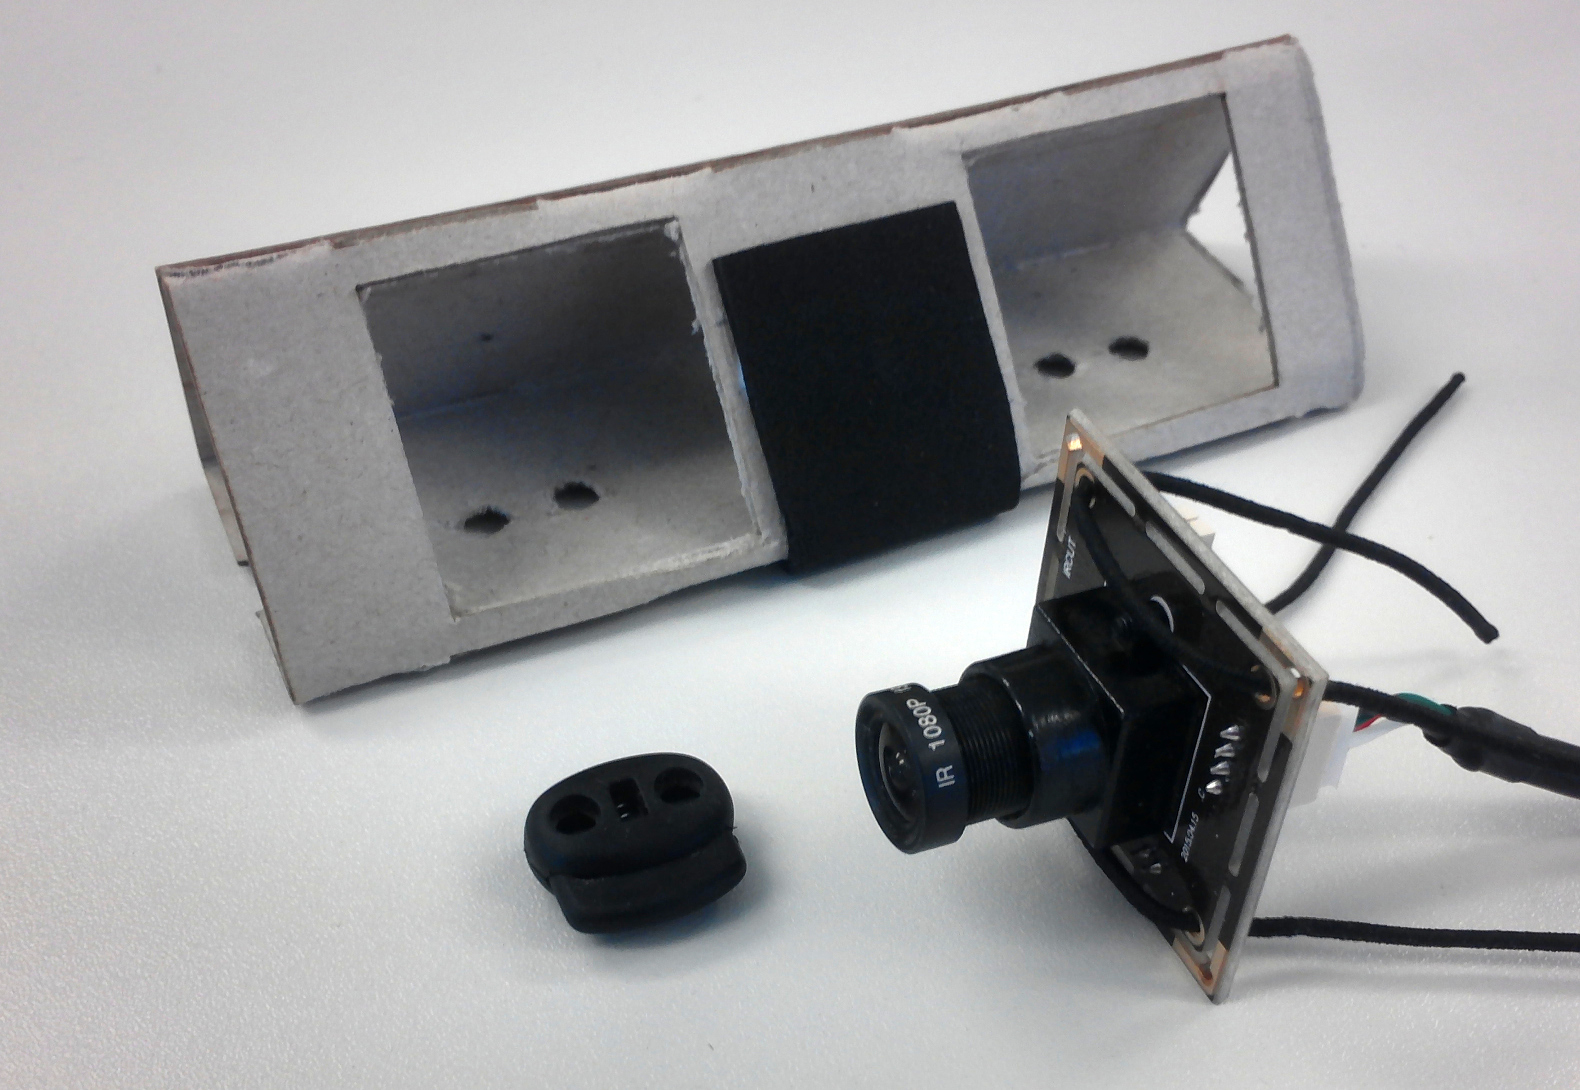
\includegraphics[width=0.7\linewidth]{holder03}
		\caption{Camera attached on part B}
		\label{fig:holder3}
	\end{figure}
	\begin{figure}[htb]
		\centering
		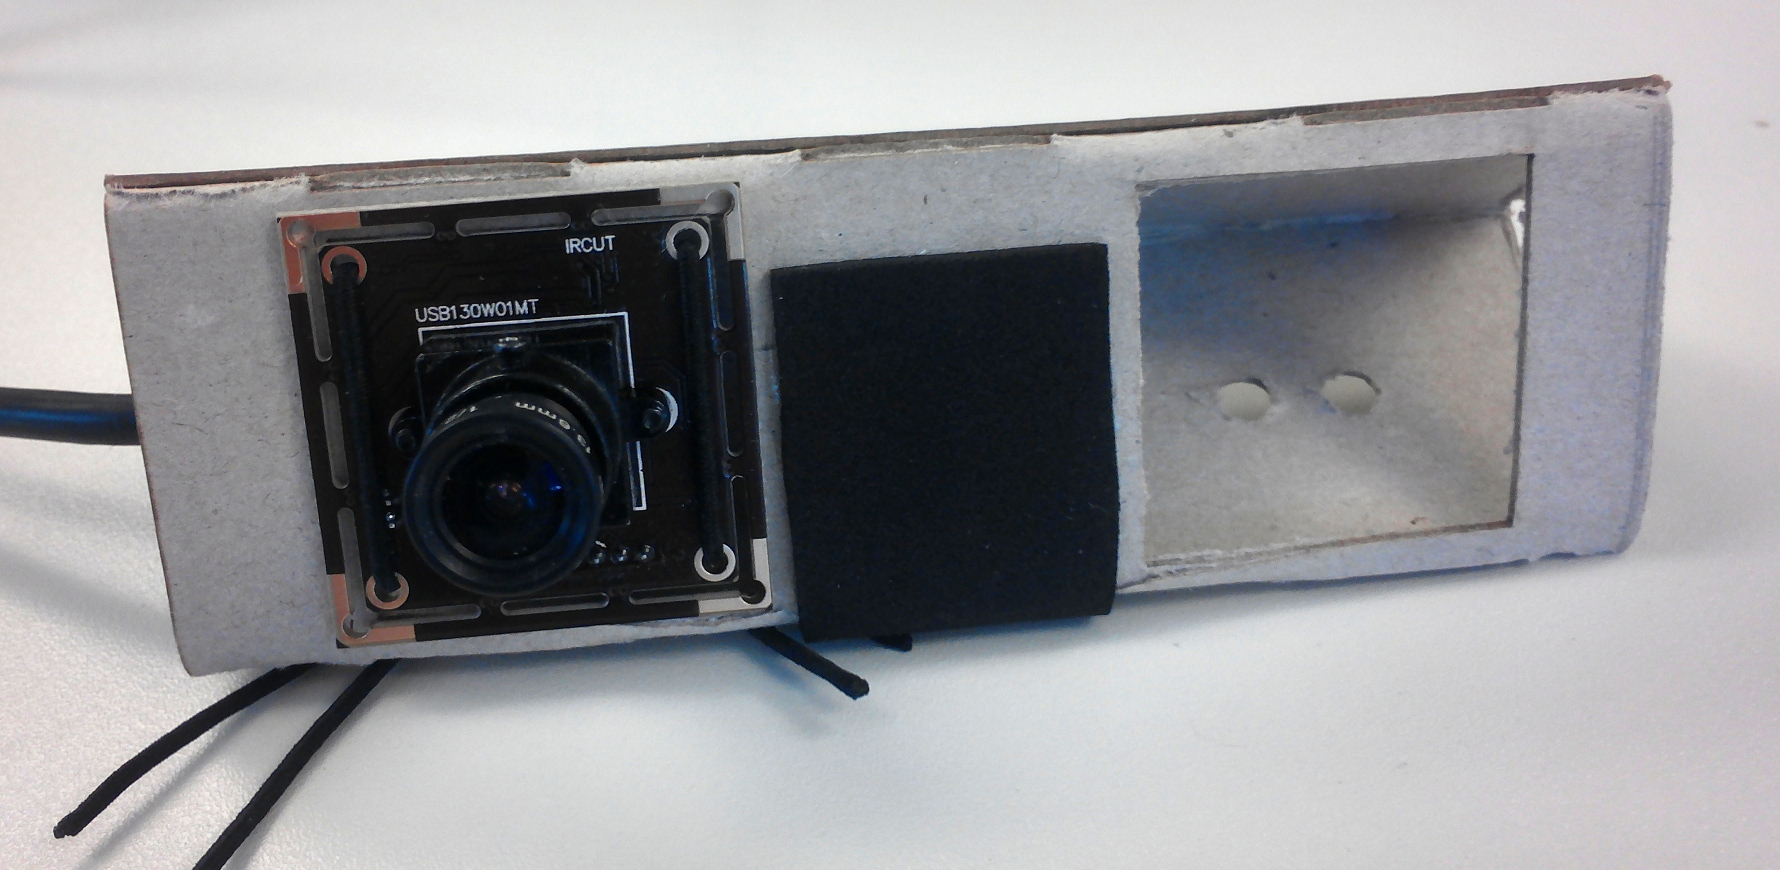
\includegraphics[width=0.55\linewidth]{holder04}\\ \vspace{2mm}
		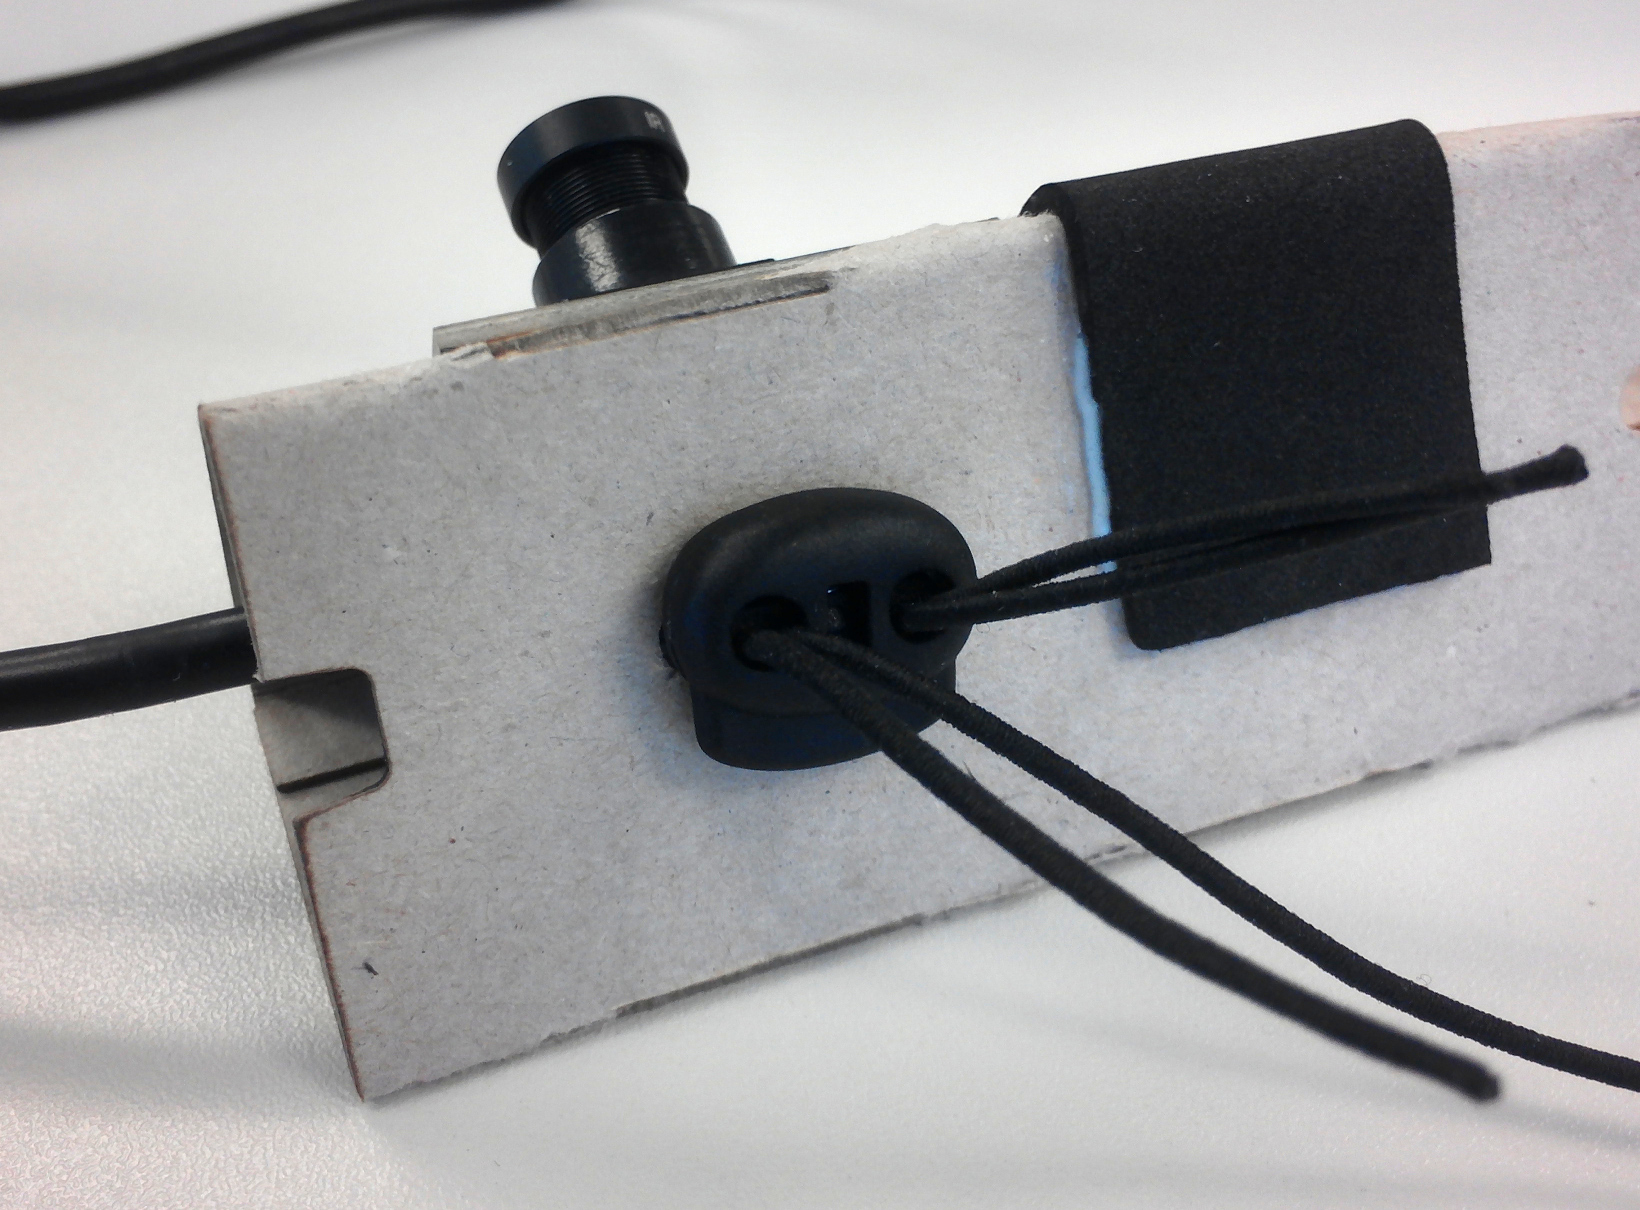
\includegraphics[width=0.55\linewidth]{holder05}
		\caption{Camera attached on part B}
		\label{fig:screenshot023}
	\end{figure}
	\clearpage
	\item Now take the camera and a screwdriver. In this step you have to adjust the focus of the camera for the short distance. This is necessary because the camera image of the eye need to be sharp for easier pupil detection in Pupil Capture. The focus of the camera we used, the \textit{ELP 960P HD 1.3 MP}, can be set by release the screw on the objective and turn the objective with the clockwise direction till the focal point is at a distance of $25$ to $30 mm$. Figure \ref{fig:setfocalpoint} visualize this process and figure \ref{fig:focalimage} shows the camera image before (left) and after (right) setting the focal point.
	\begin{figure}[h!tb]
		\centering
		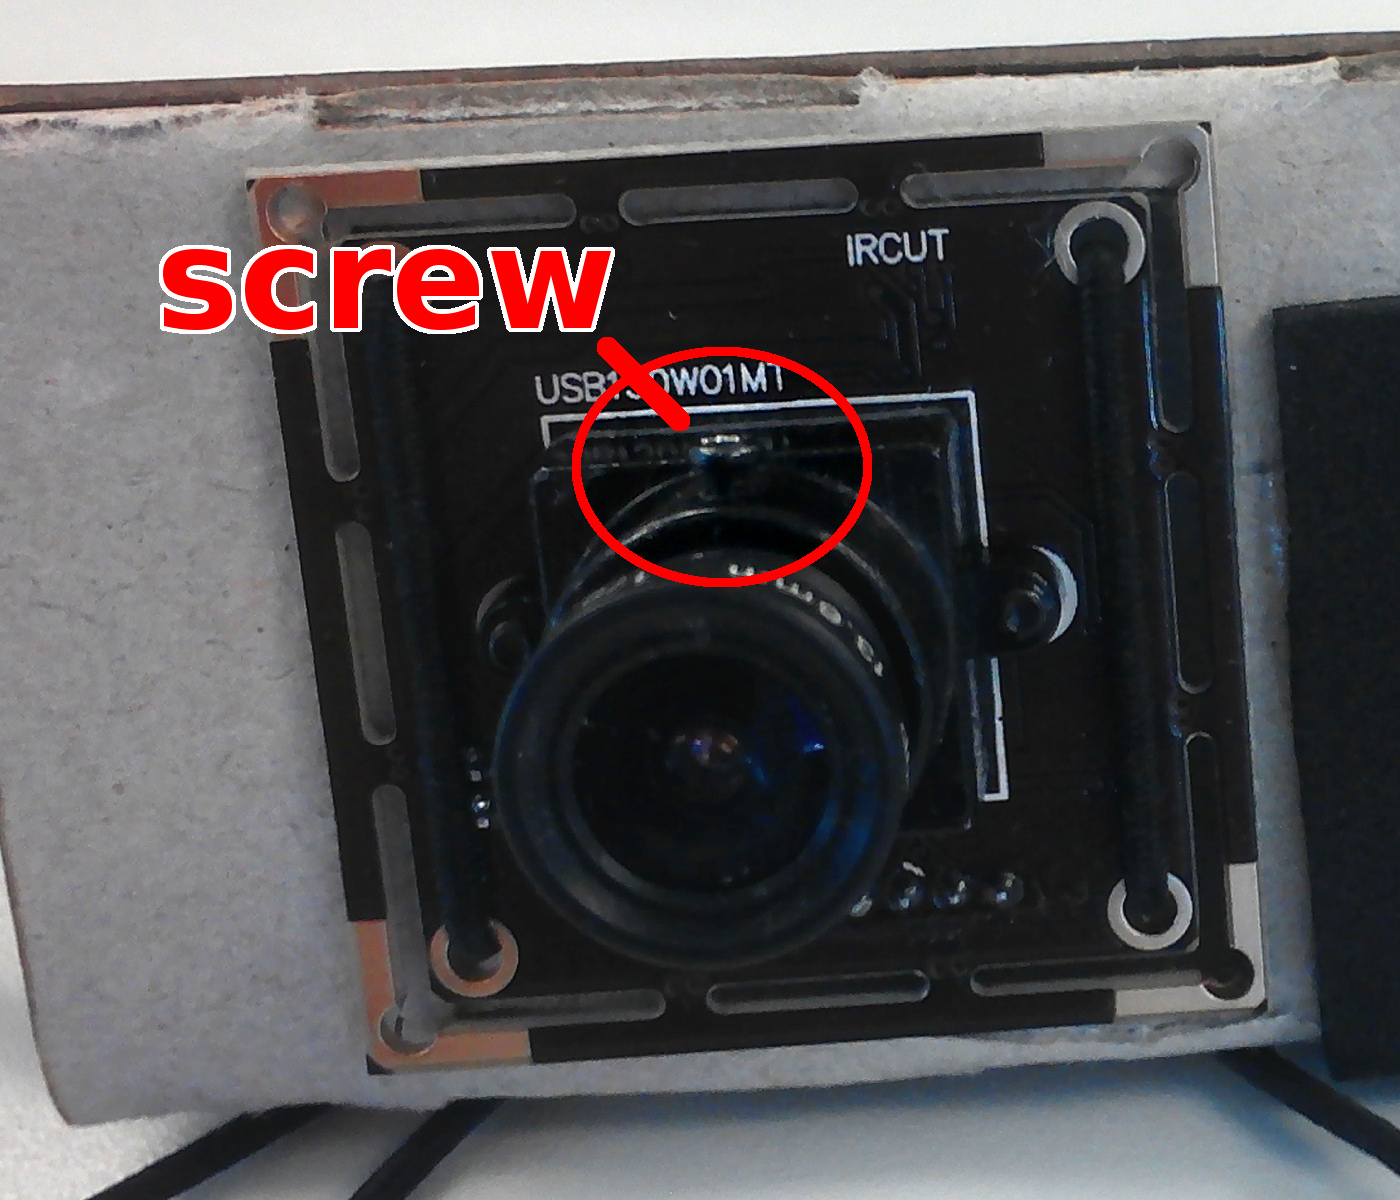
\includegraphics[width=0.3\linewidth]{holder06}
		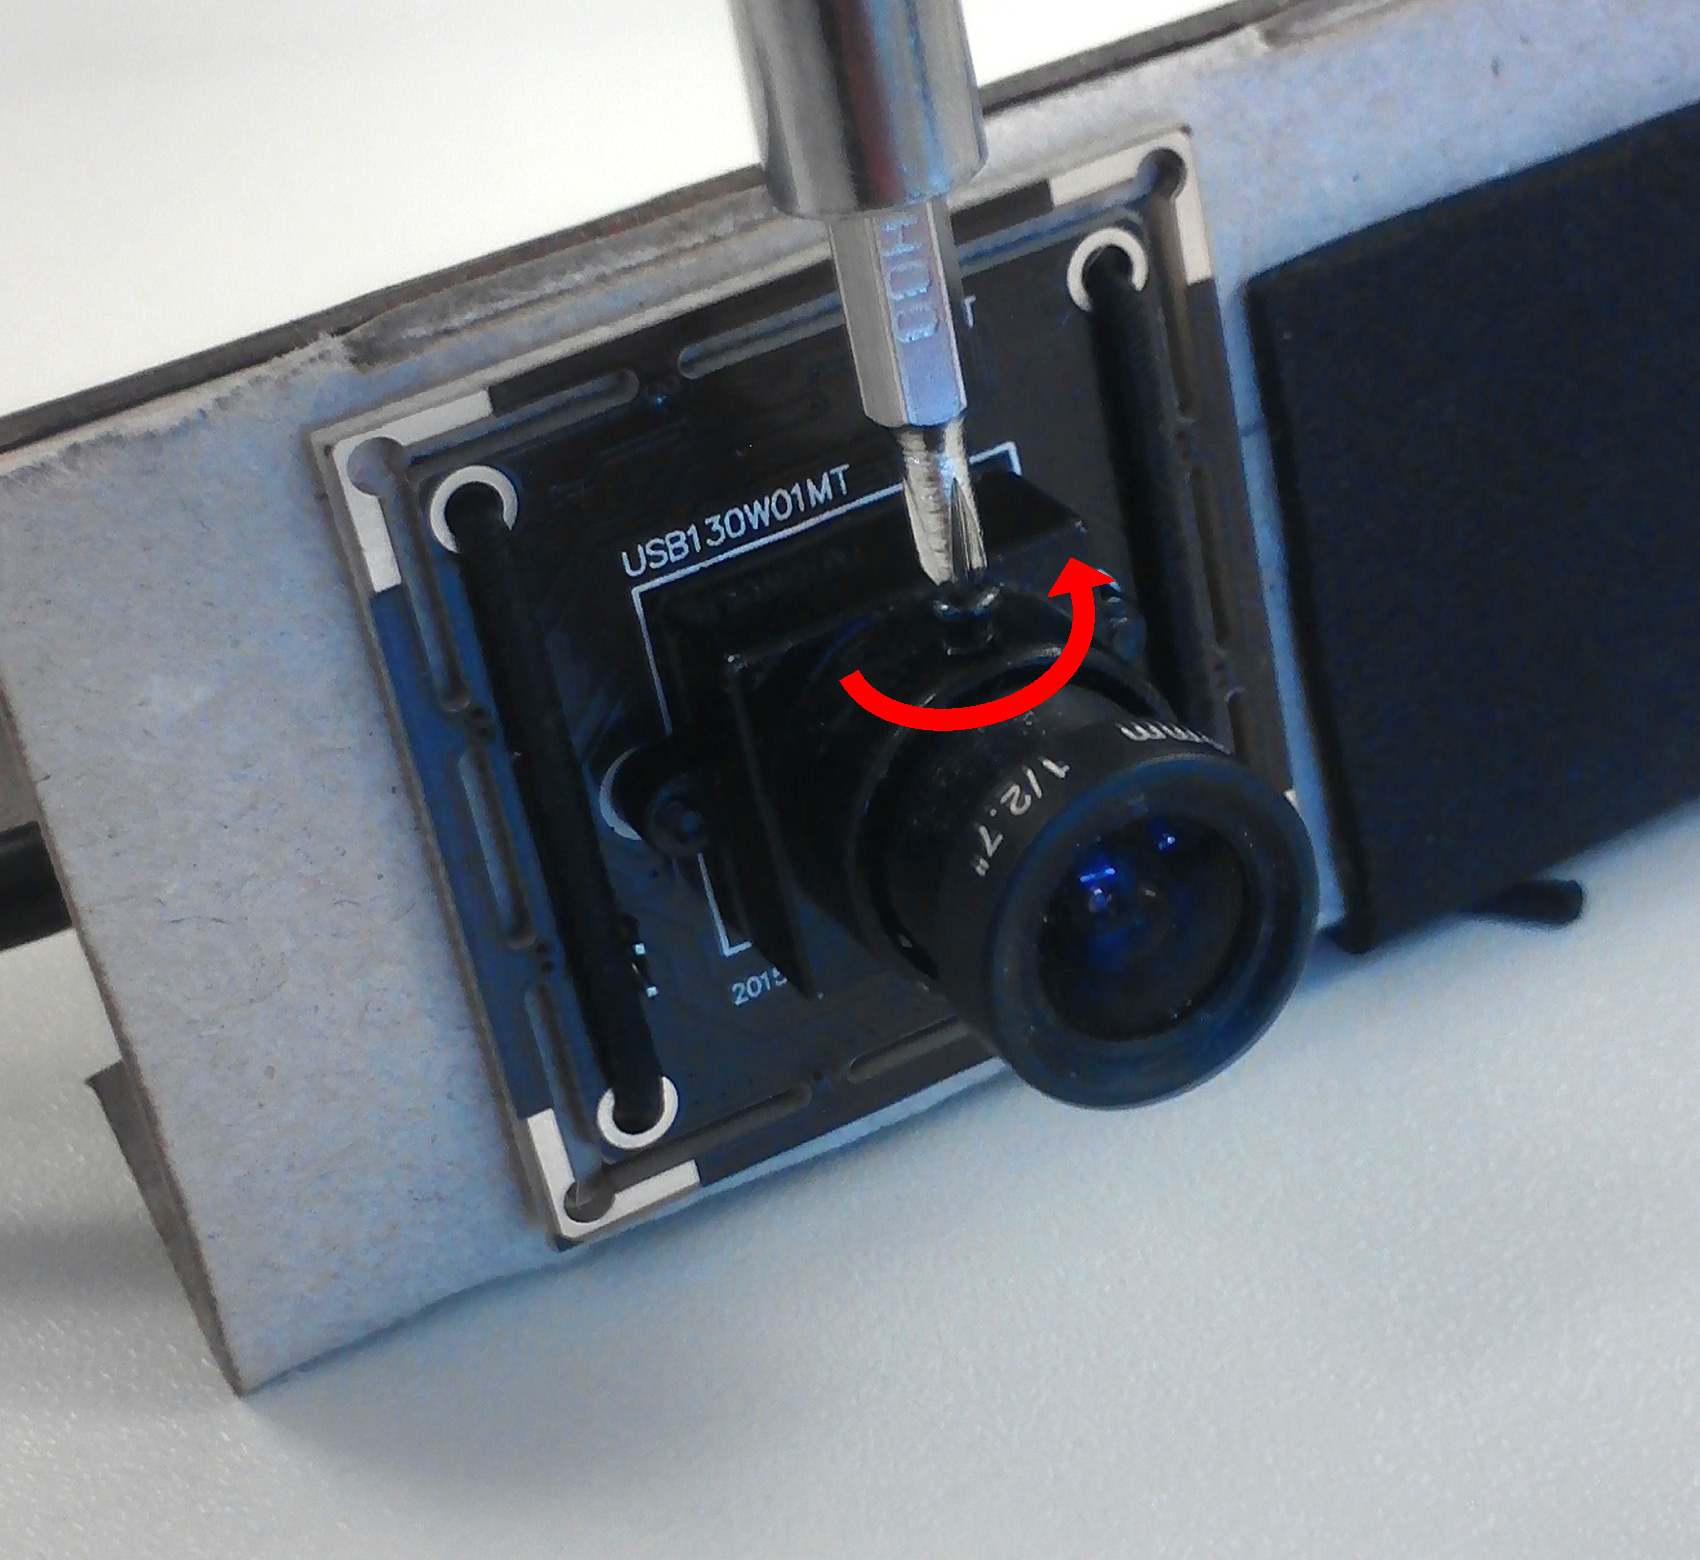
\includegraphics[width=0.3\linewidth]{holder07}\\ \vspace{0.1cm}
		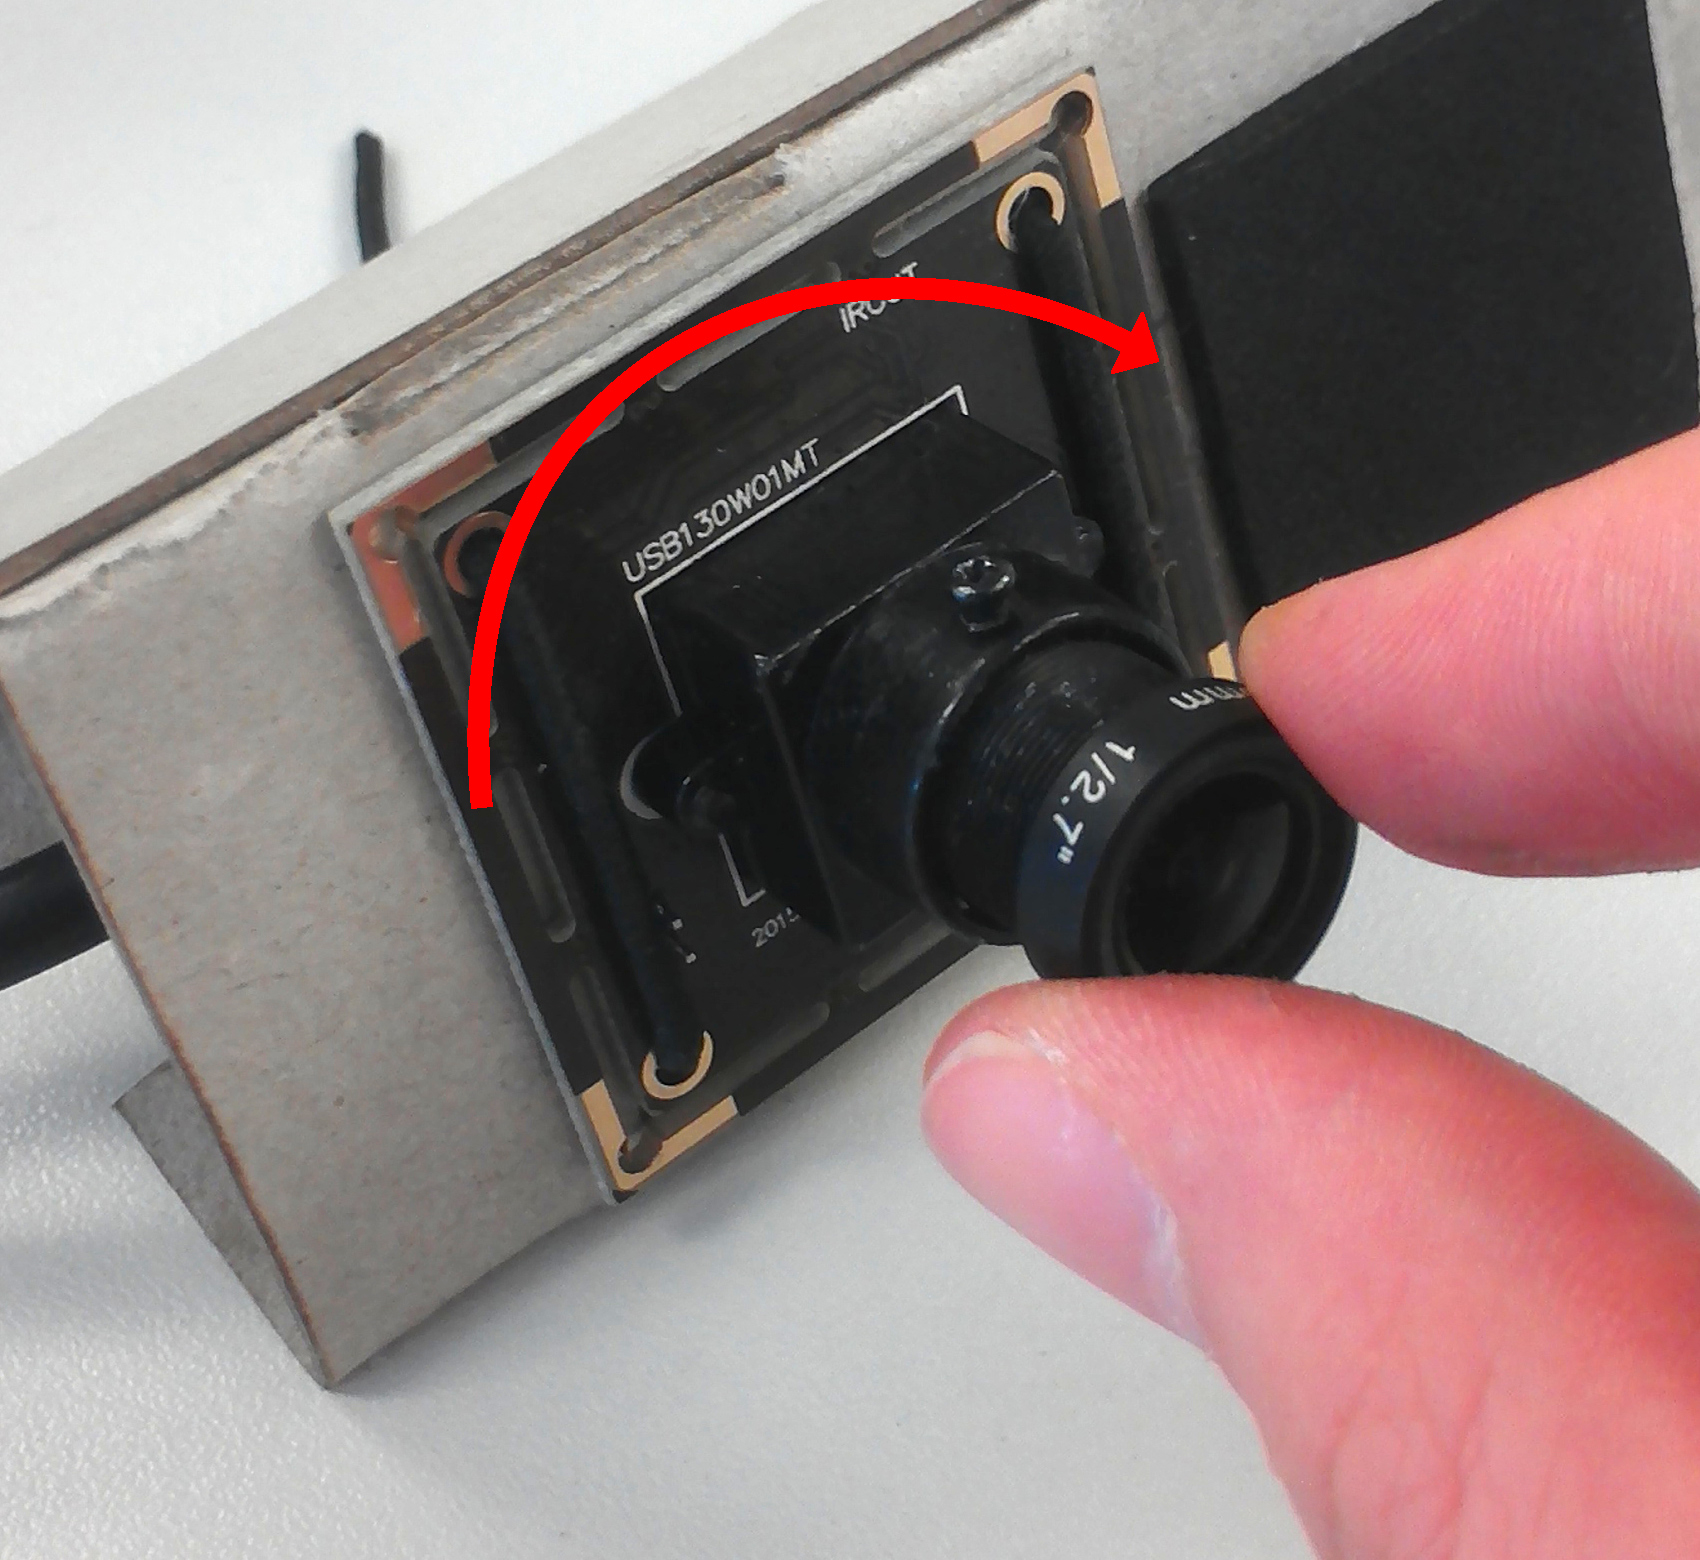
\includegraphics[width=0.3\linewidth]{holder08}
		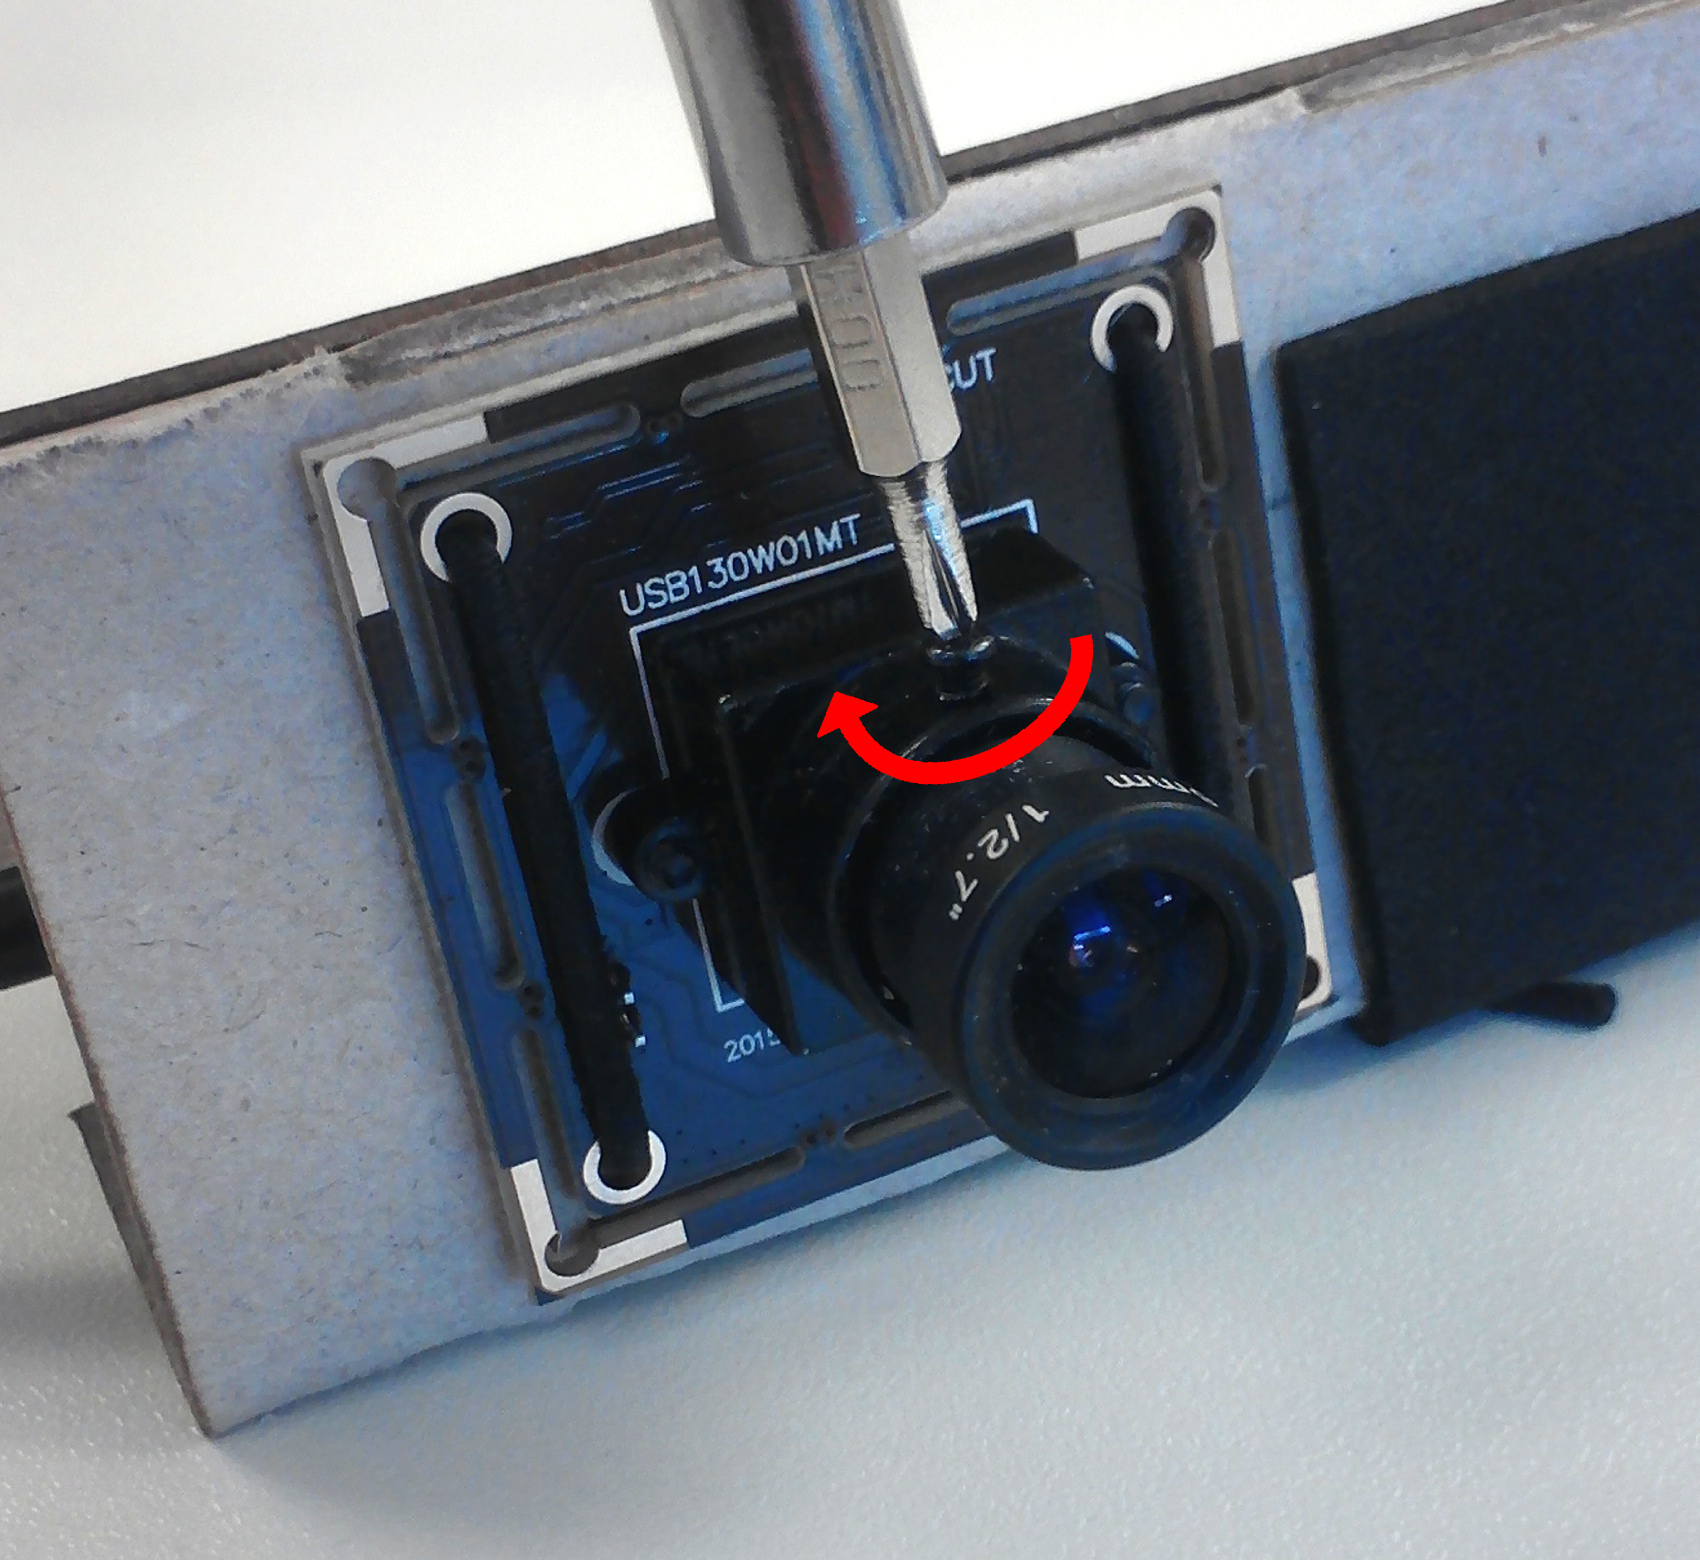
\includegraphics[width=0.3\linewidth]{holder09}
		\caption{Setting the focal point on an ELP 960P HD 1.3 MP}
		\label{fig:setfocalpoint}
	\end{figure}
	\begin{figure}[htb]
		\centering
		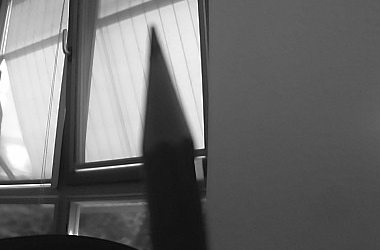
\includegraphics[width=0.39\linewidth]{FokusKamera01}
		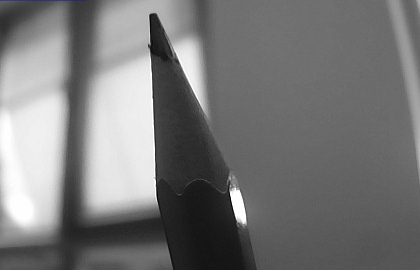
\includegraphics[width=0.4\linewidth]{FokusKamera02}
		\caption{Camera image before (left) and after (right) setting the focal point correctly}
		\label{fig:focalimage}
	\end{figure}
	
	\item The next step is to place the circuit board on the camera (see figure \ref{fig:holder10}). It's recommended to place some hot glue on the bottom-side of the circuit board to prevent short circuit. Then attach the circuit board on the camera. To do this rotate the circuit board 45 degrees to pull it over the screw of the camera and then rotate it back like in figure \ref{fig:holder12}.
	\begin{figure}[htb]
		\centering
		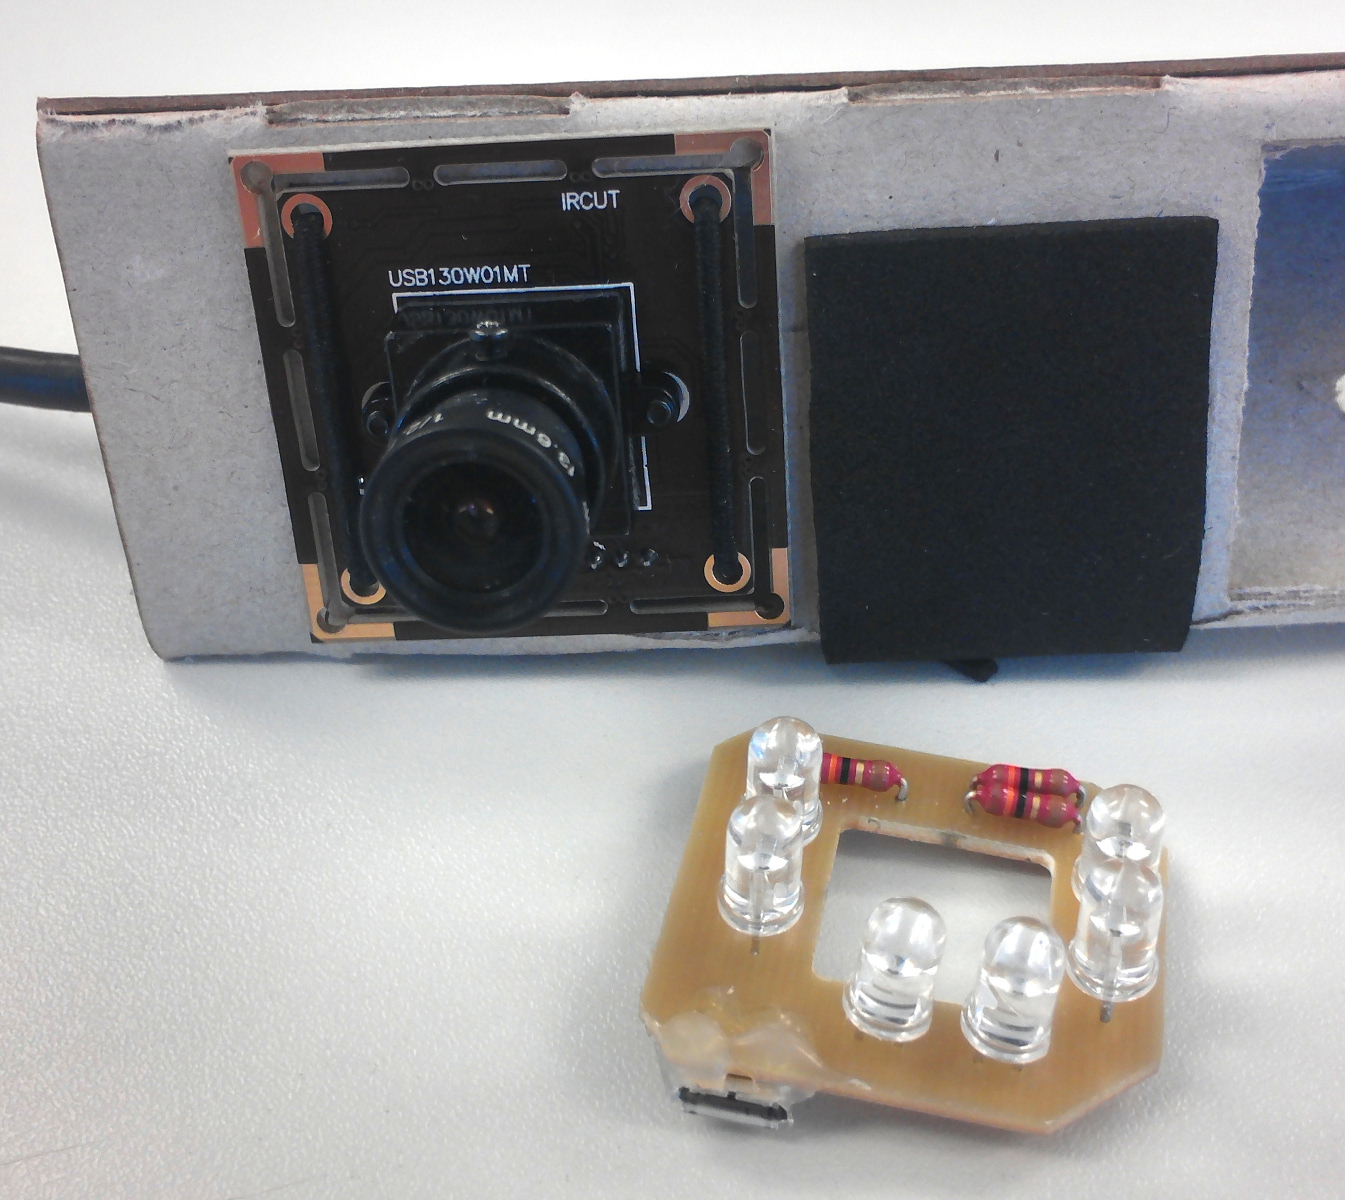
\includegraphics[width=0.55\linewidth]{holder10}
		\caption{Circuit board and the camera}
		\label{fig:holder10}
	\end{figure}
	\begin{figure}[htb]
		\centering
		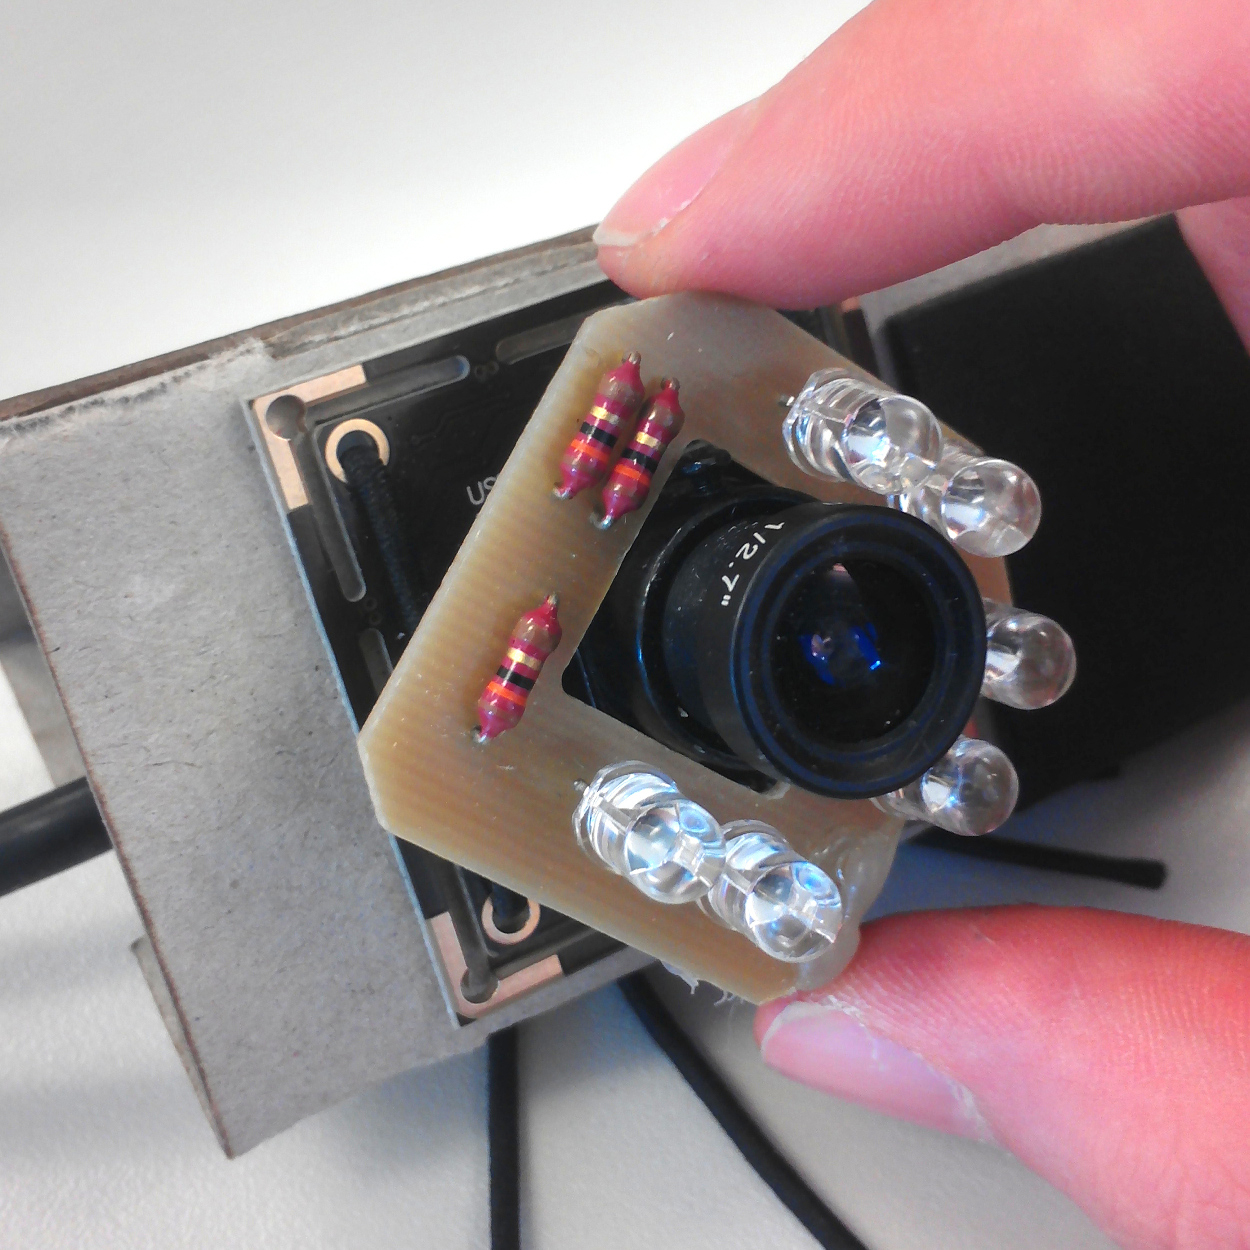
\includegraphics[width=0.38\linewidth]{holder11}
		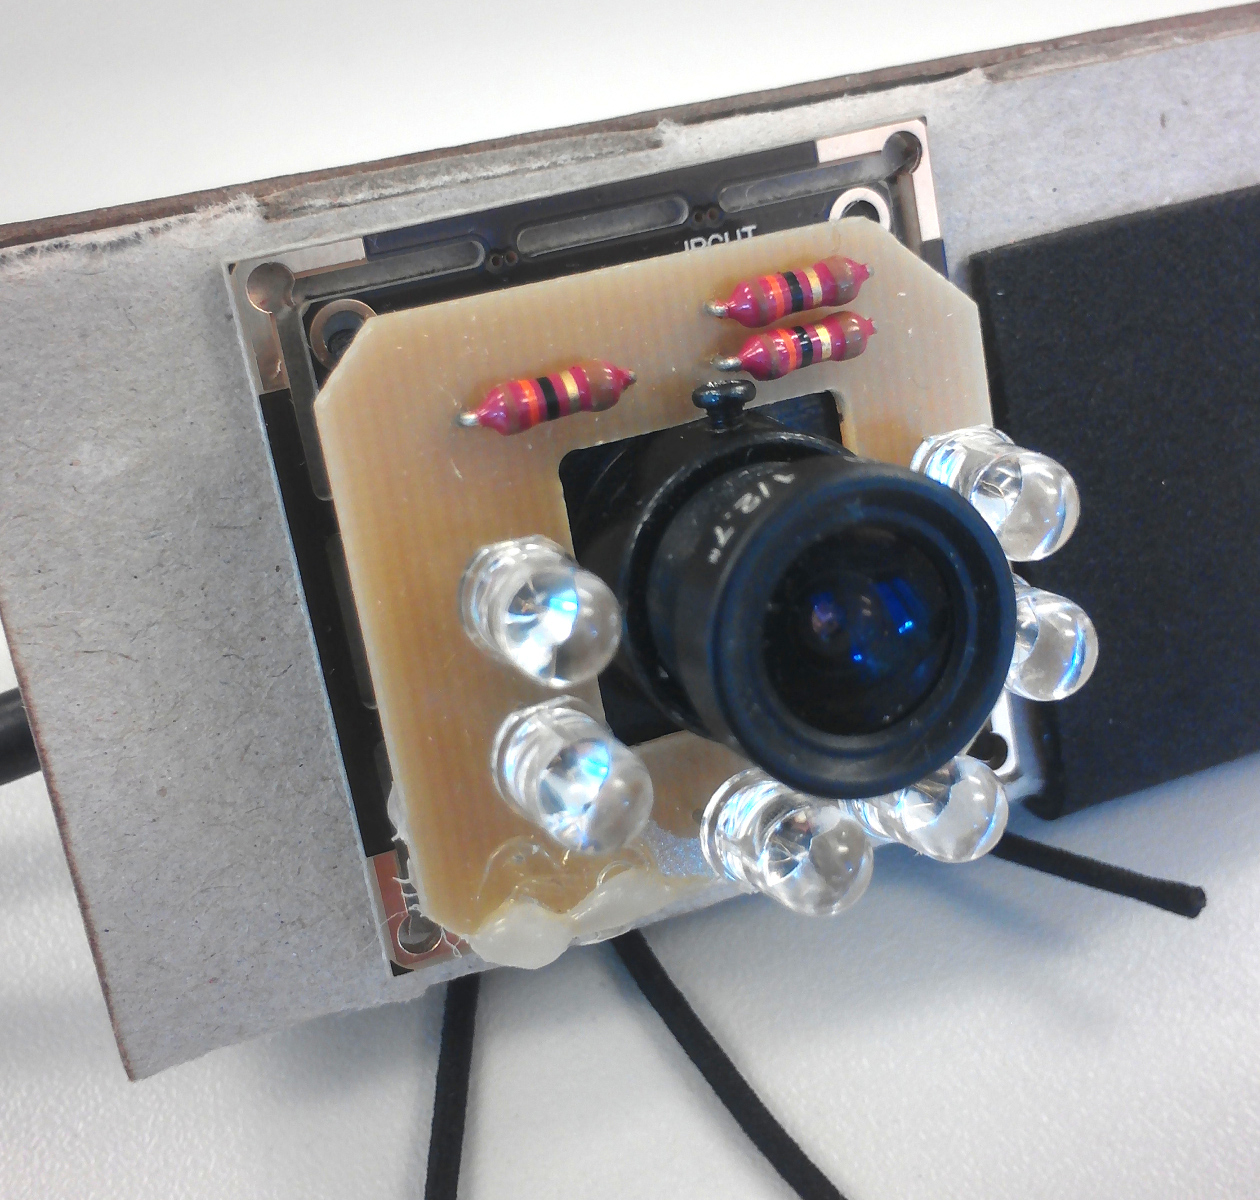
\includegraphics[width=0.4\linewidth]{holder12}
		\caption{Attaching the circuit board on the camera}
		\label{fig:holder12}
	\end{figure}
	\clearpage
	\item Finally, glue the part B with hot glue into the cardboard. The bottom edge of part B should fit the marked line inside the cardboard. The camera objective should be centered under the lens, like shown in figure \ref{fig:objective}. The result should look like on figure \ref{fig:screenshot024}.
	\begin{figure}[h!tb]
		\centering
		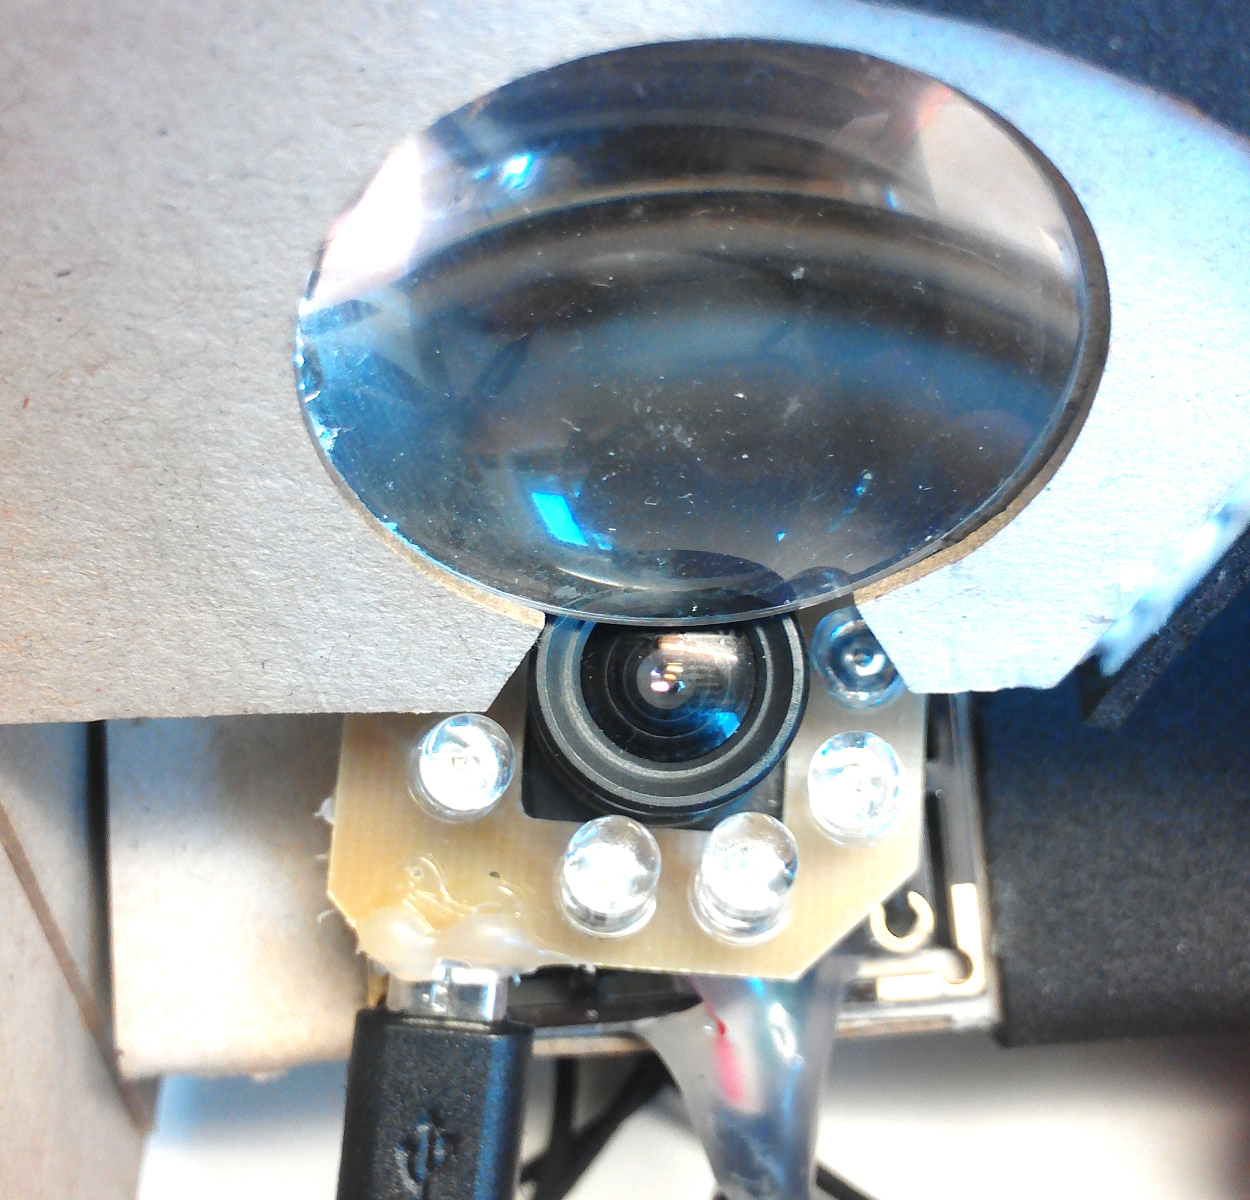
\includegraphics[width=0.45\linewidth]{positionObj}
		\caption{Objective of the camera is centered under the lens}
		\label{fig:objective}
	\end{figure}
	\begin{figure}[h!tb]
		\centering
		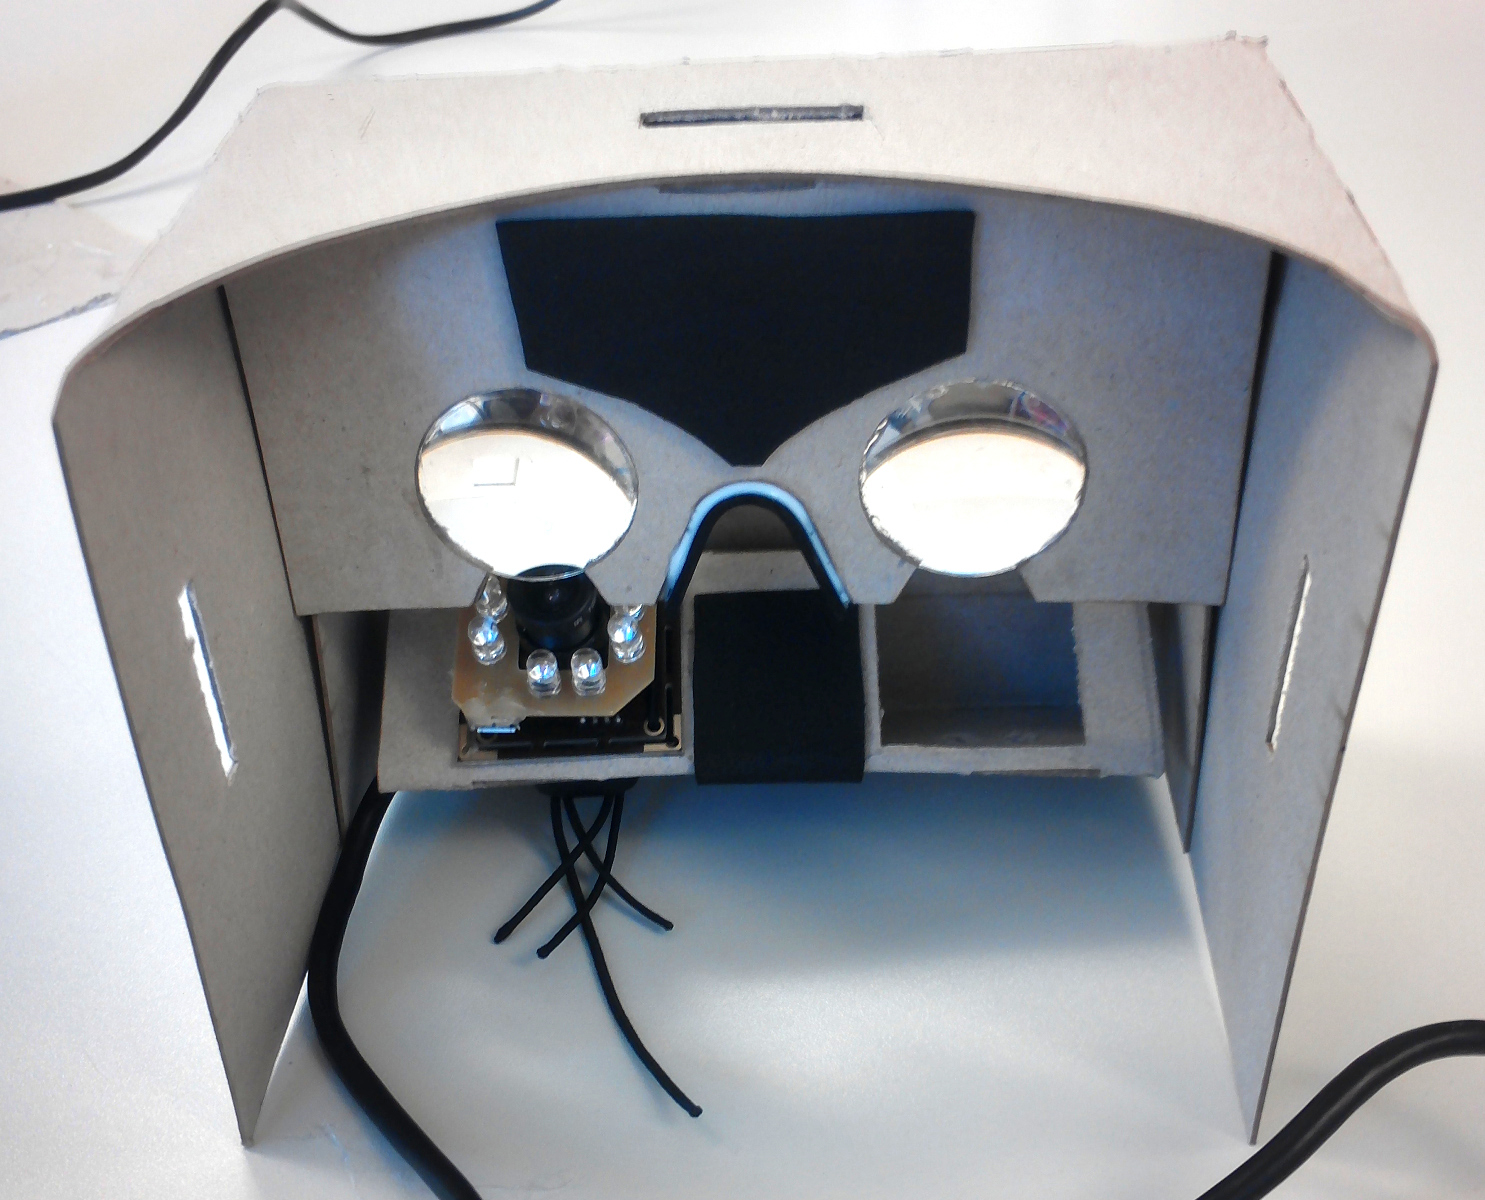
\includegraphics[width=0.65\linewidth]{holder13}
		\caption{Cardboard with camera and board as well as the attachment}
		\label{fig:screenshot024}
	\end{figure}
	\clearpage
	\item For the next step, take the Velcro rubber bands and two male Velcro tapes (see figure \ref{fig:head1}). Sew on each end of the female Velcro rubber bands a male Velcro tape.
	\begin{figure}[h!tb]
		\centering
		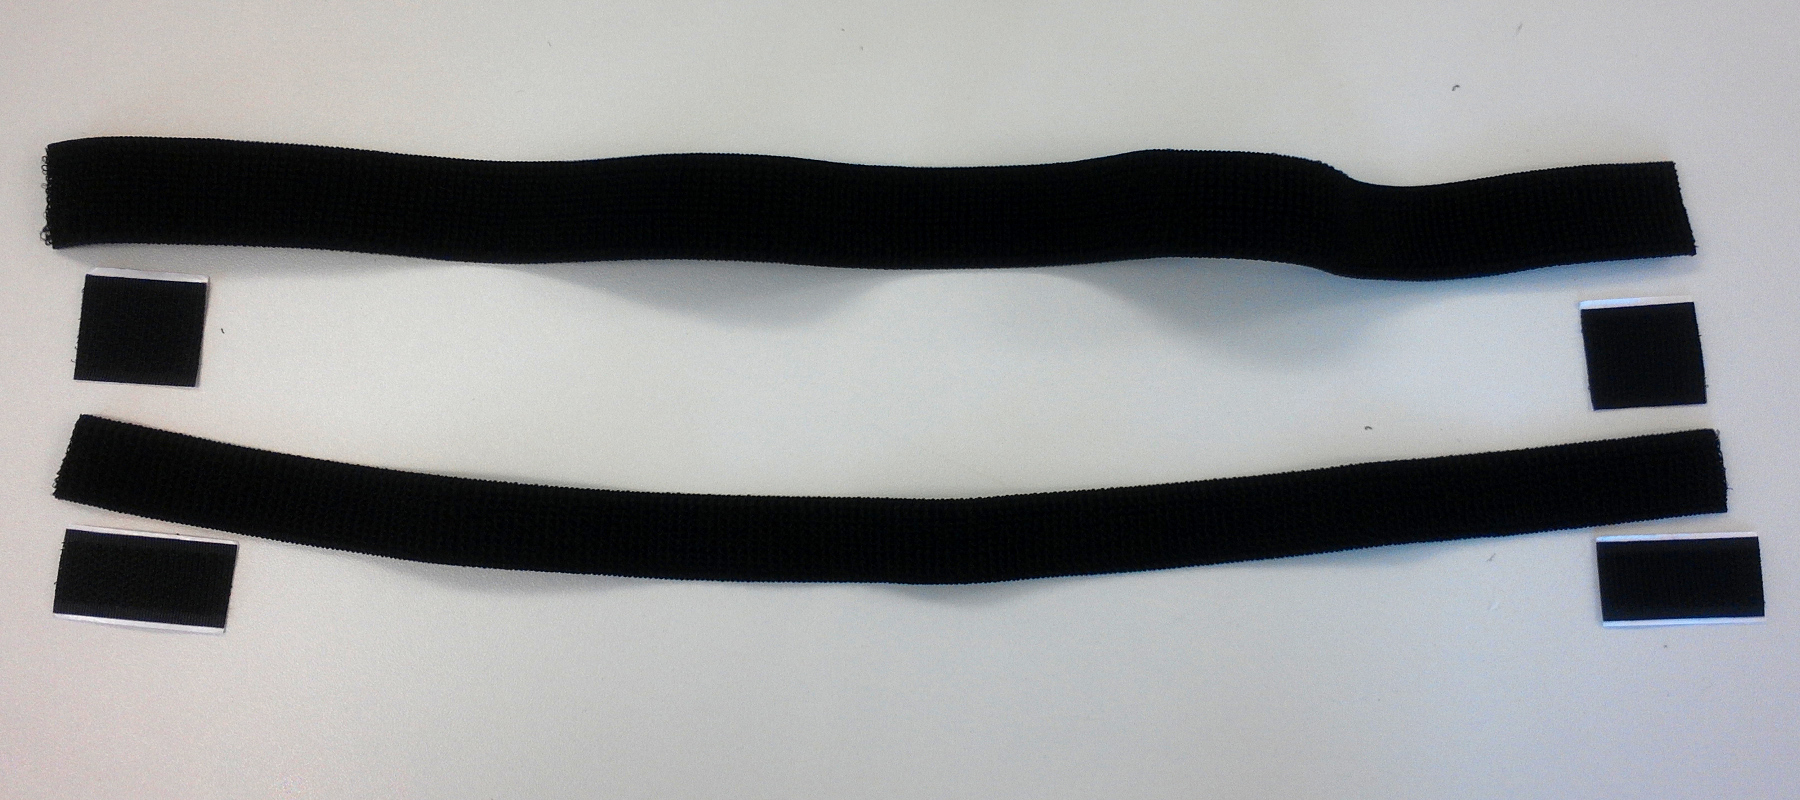
\includegraphics[width=0.63\linewidth]{head01}
		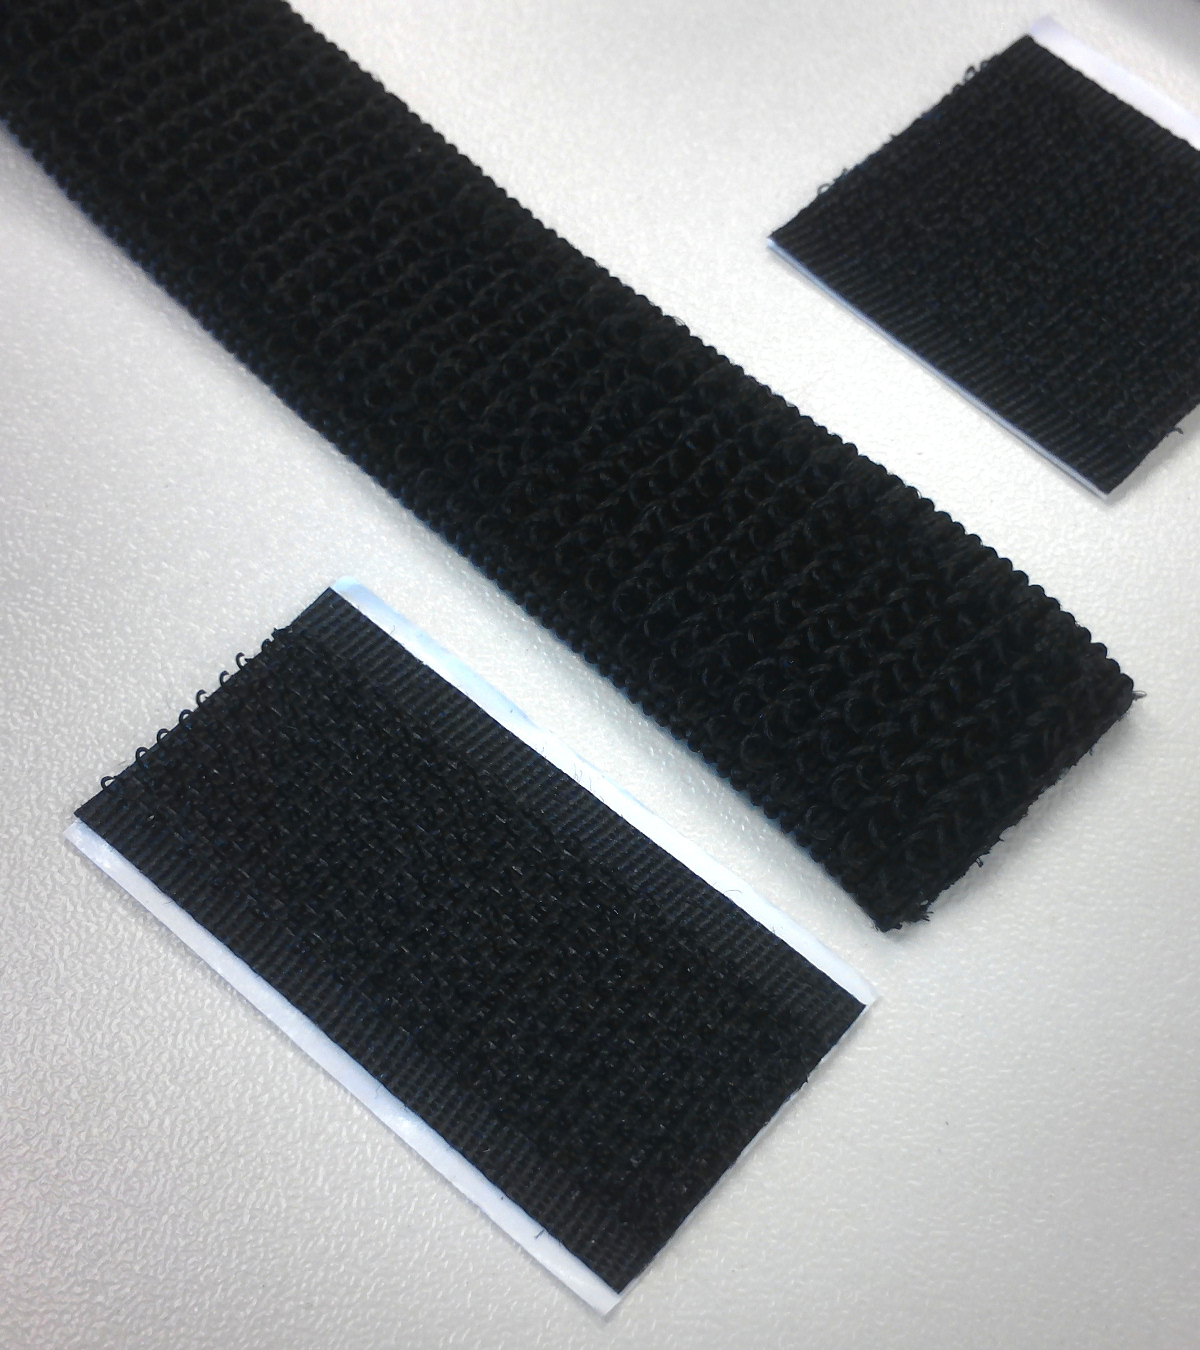
\includegraphics[width=0.25\linewidth]{head02}
		\caption{Female Velcro rubber bands and male Velcro tapes}
		\label{fig:head1}
	\end{figure}
	\item Now take one Velcro rubber band attach one end to the left slot of the cardboard, as shown in figure \ref{fig:screenshot025}. Then pull the other end of the Velcro rubber band though the right slot of the cardbard, as shown in figure \ref{fig:head5}. The result should looks like on the figure \ref{fig:screenshot026}.	
	\begin{figure}[h!tb]
		\centering
		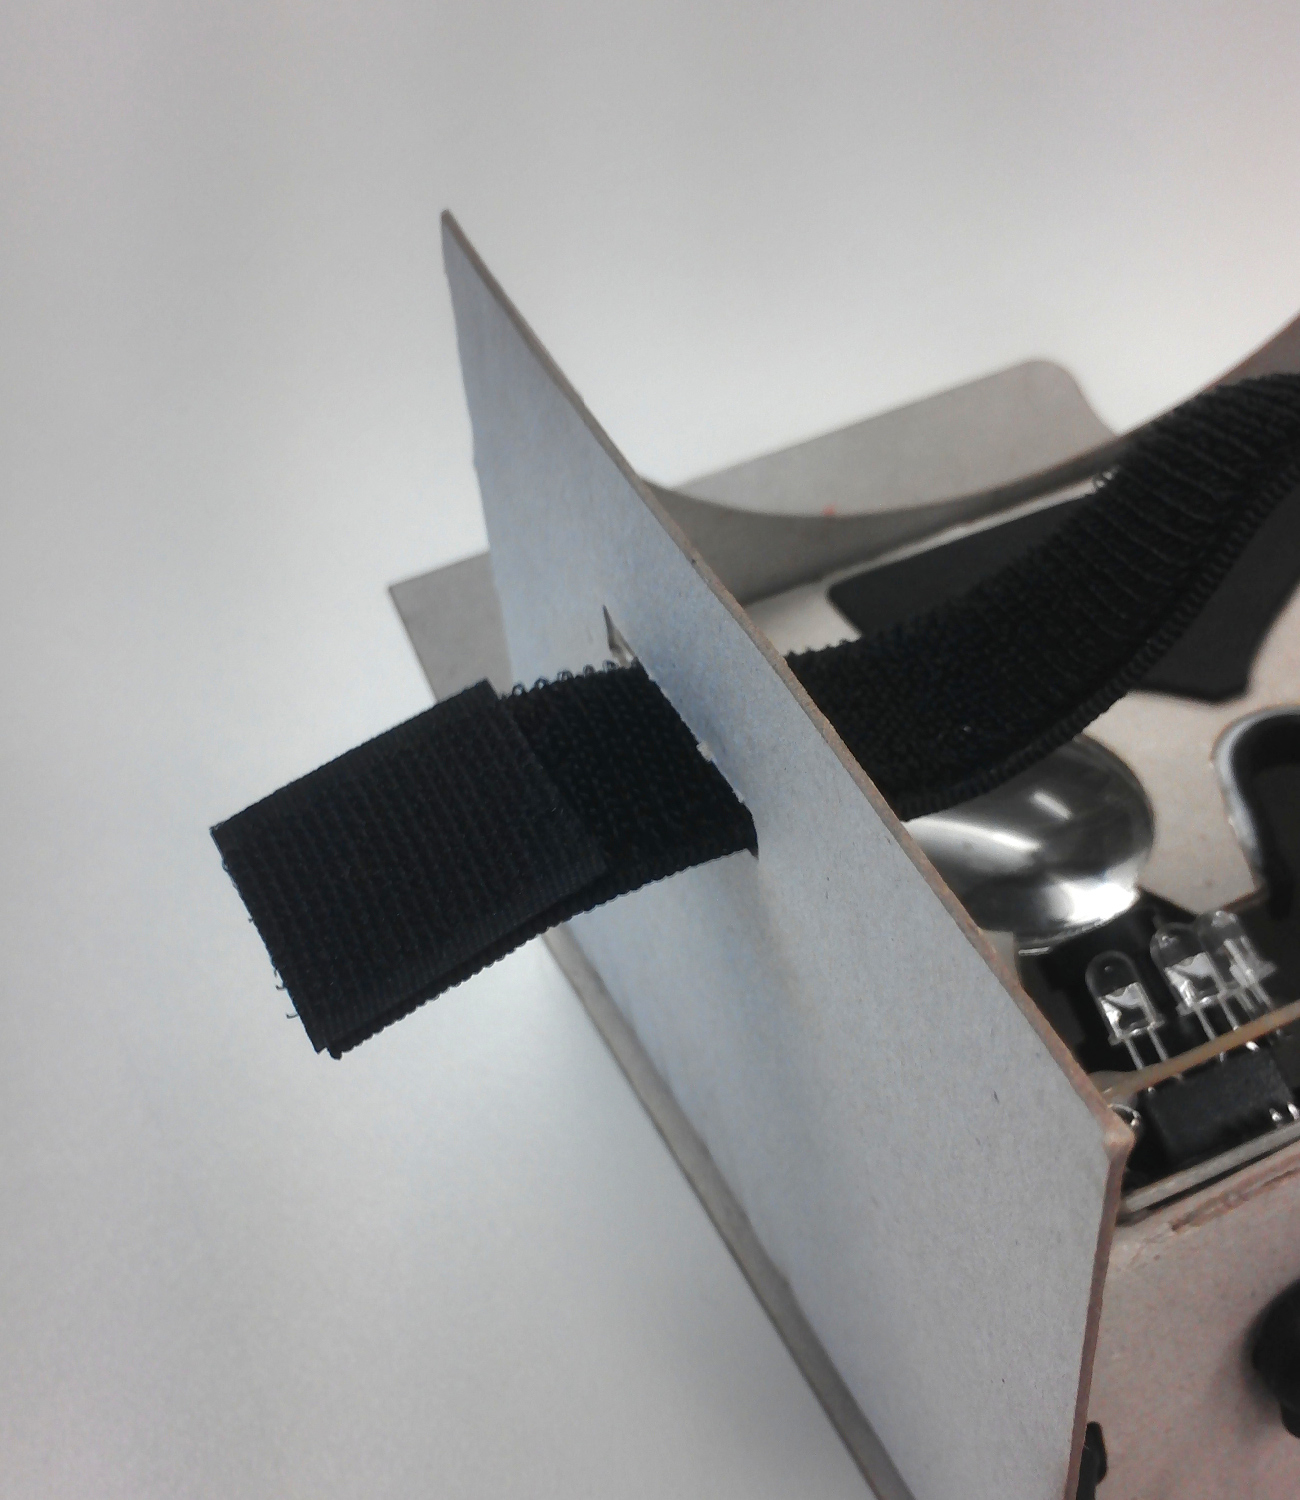
\includegraphics[width=0.4\linewidth]{head05}
		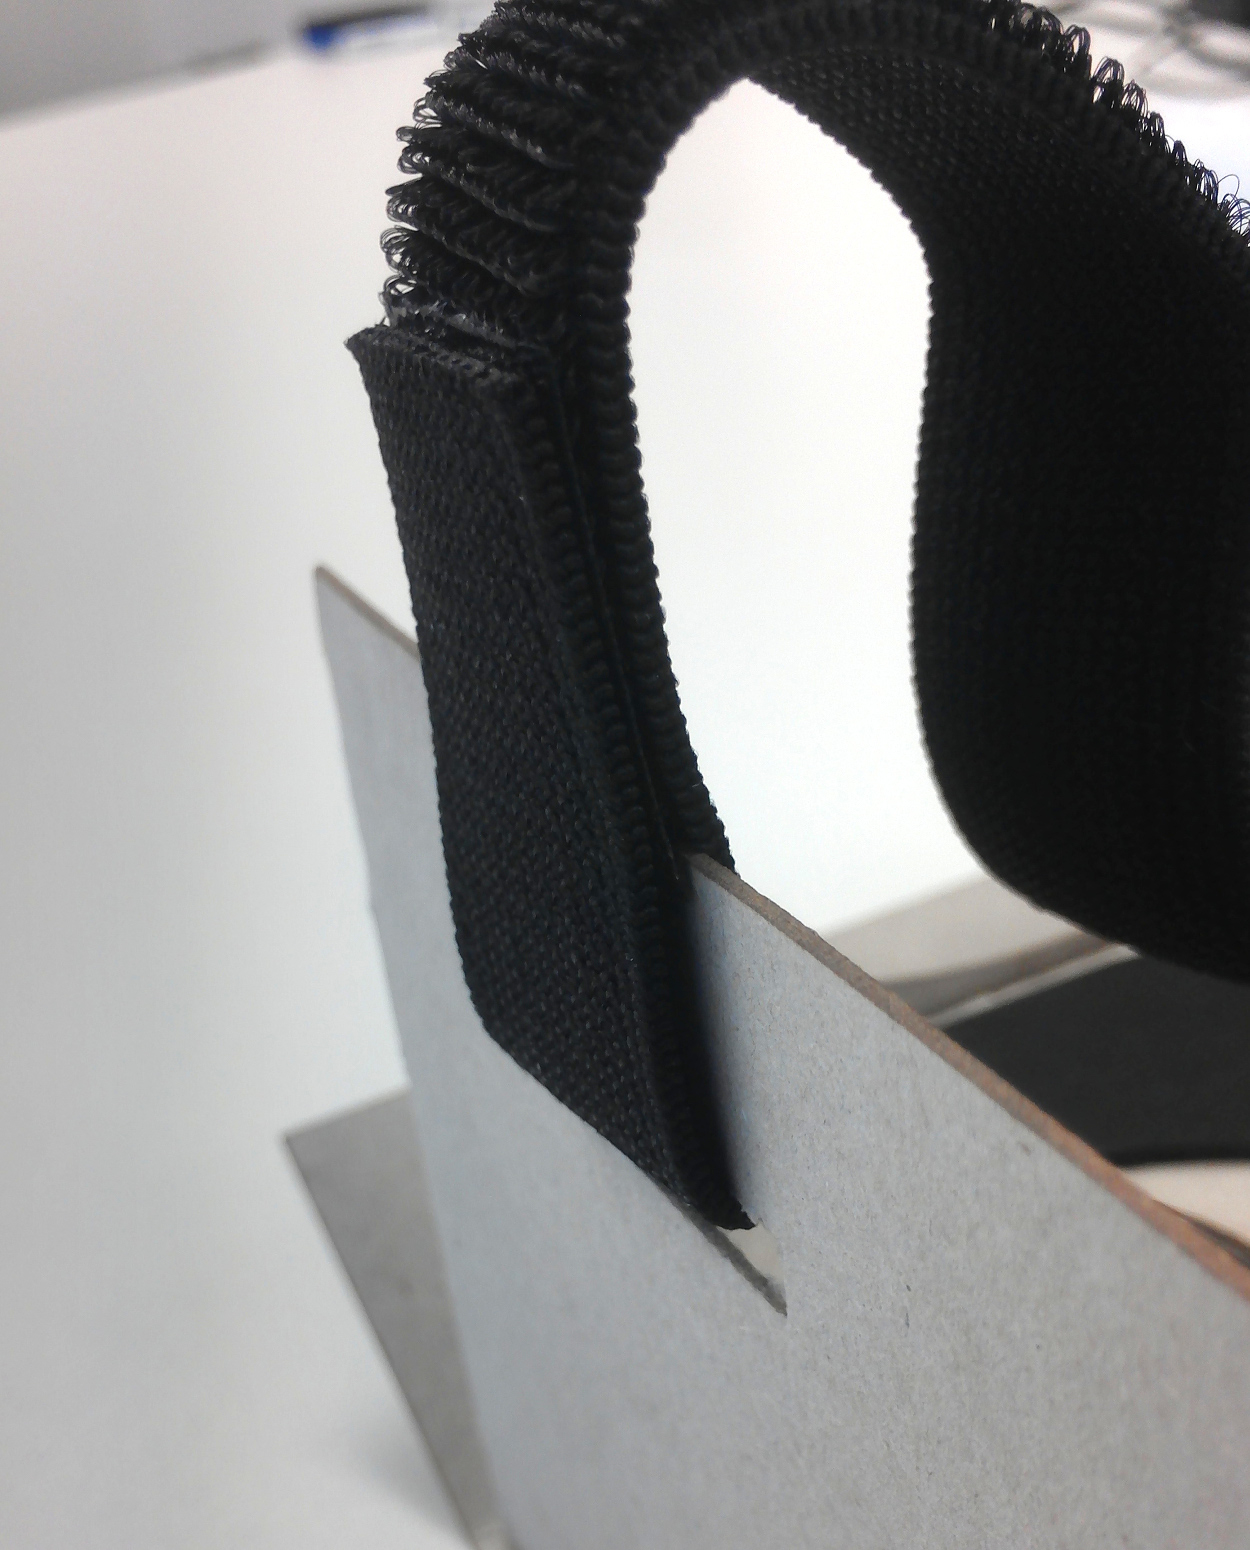
\includegraphics[width=0.37\linewidth]{head06}
		\caption{Attach the rubber band on the left side of the cardboard}
		\label{fig:screenshot025}
	\end{figure}
	\begin{figure}[h!tb]
		\centering
		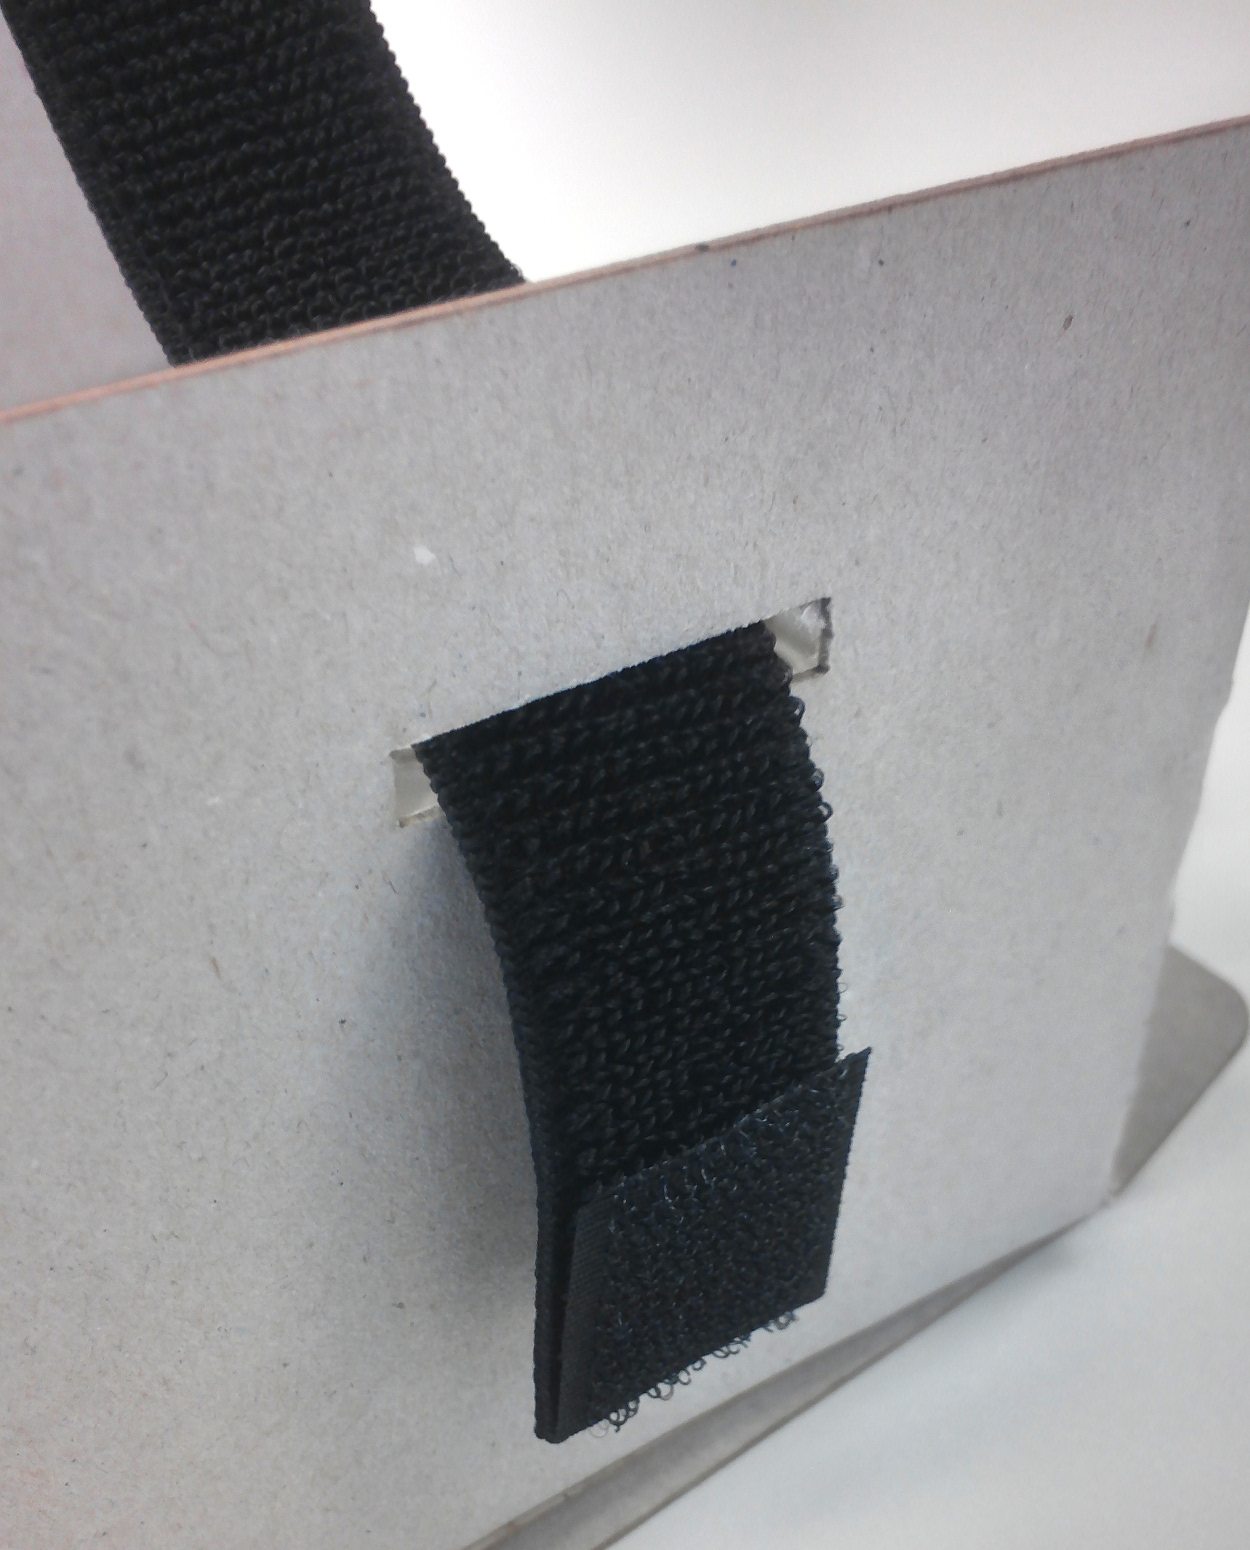
\includegraphics[width=0.33\linewidth]{head03}
		\includegraphics[width=0.33\linewidth]{head04}
		\caption{Attach the rubber band on the right side of the cardboard}
		\label{fig:head5}
	\end{figure}
	\begin{figure}[h!tb]
		\centering
		\includegraphics[width=0.6\linewidth]{head07}
		\caption{Cardboard with one attached Velcro rubber band}
		\label{fig:screenshot026}
	\end{figure}
	\clearpage
	\item Take the second Velcro rubber band and attach it's end to the top slot of the card board, shown in figure \ref{fig:screenshot027}. As final step take the other end and surround the first rubber band with the second, as shown in figure \ref{fig:screenshot028}, to complete the head mount.
	\begin{figure}[h!tb]
		\centering
		\includegraphics[width=0.33\linewidth]{head08}
		\includegraphics[width=0.33\linewidth]{head09}
		\caption{Attach the second rubber band to the top of the cardboard}
		\label{fig:screenshot027}
	\end{figure}
	\begin{figure}[h!tb]
		\centering
		\includegraphics[width=0.55\linewidth]{head10}
		\caption{Attach the other end to the first rubber band}
		\label{fig:screenshot028}
	\end{figure}
\item As the next step take one male and one female Velcro tapes (see figure \ref{fig:flap01}). Glue one tape on the top of the cardboard and it's counterpart on the end of the flap of the cardboard, as shown in figure \ref{fig:flap02}. It's important that the position of both tapes have to match when the flap is closed, else the flap won't stay closed.
\begin{figure}[htb]
		\centering
		\includegraphics[width=0.53\linewidth]{flap01}
		\caption{male (left) and female (right) Velcro tapes}
		\label{fig:flap01}
\end{figure}
\begin{figure}[htb]
		\centering
		\includegraphics[width=0.5\linewidth]{flap02}
		\caption{Glueing the tapes onto the cardboard}
		\label{fig:flap02}
	\end{figure}	
	\clearpage
 \item You can now take a 4-port USB-hub and insert it under part F inside the flap of the cardboard, like shown in figure \ref{fig:hub}. The ports should look to the bottom. Finally, take (micro)USB cables to connect the camera and the circuit board with the hub.	
\end{enumerate}
\begin{figure}[htb]
		\centering
		\includegraphics[width=0.6\linewidth]{hubPosition}
		\caption{Position of 4-port USB-hub inside the flap}
		\label{fig:hub}
	\end{figure}	
If you followed the guide correctly, you should now have a cardboard which looks like the one on the figure \ref{fig:screenshot030} and \ref{fig:screenshot031}. 
\begin{figure}[htb]
		\centering
		\includegraphics[width=0.5\linewidth]{finalCardboard01}
		\caption{The inside of the resultant cardboard}
		\label{fig:screenshot030}
\end{figure}
\begin{figure}[htb]
		\centering
		\includegraphics[width=0.55\linewidth]{finalCardboard02}\\ \vspace{1mm}
		\includegraphics[width=0.55\linewidth]{finalCardboard03}
		\caption{The outside of the resultant cardboard}
		\label{fig:screenshot031}
	\end{figure}
\end{document}